% ===========================================================================
%  Laporan teknis paket R fastsae
%  Sumber klaim : kode paket (R/, src/, man/, vignettes/, tests/, inst/)
%  Sumber angka : inst/extdata/*.rds lewat scripts/*.R  (tidak ada angka manual)
%  Bahasa       : Indonesia
%  Build        : latexmk -pdf main.tex     (lihat .latexmkrc)
% ===========================================================================
\documentclass[11pt,a4paper]{article}

% ---- dasar teks -----------------------------------------------------------
\usepackage[T1]{fontenc}
\usepackage[utf8]{inputenc}
\usepackage{lmodern}
\usepackage[english,bahasa]{babel}

% ---- matematika & tabel ---------------------------------------------------
\usepackage{amsmath,amssymb,amsthm}
\usepackage{booktabs}
\usepackage{tabularx}
\usepackage{multirow}
\usepackage{siunitx}

% ---- tampilan -------------------------------------------------------------
\usepackage[margin=2.6cm]{geometry}
\usepackage{graphicx}
\usepackage{xcolor}
\usepackage{caption}
\usepackage{subcaption}
\usepackage{float}
\usepackage{enumitem}
\usepackage{microtype}
\usepackage{listings}

% ---- tautan & sitasi ------------------------------------------------------
\usepackage[colorlinks=true,linkcolor=blue!50!black,citecolor=blue!50!black,
            urlcolor=blue!70!black,bookmarks=true]{hyperref}
\usepackage{natbib}
\bibliographystyle{plainnat}

% ---- algoritme (setelah hyperref) -----------------------------------------
\usepackage[ruled,vlined,linesnumbered]{algorithm2e}
\SetKwComment{KwCom}{\% }{}
\SetKw{KwIn}{Masukan}
\SetKw{KwOut}{Keluaran}
\SetKw{KwData}{Data}
\SetKw{KwRet}{kembalikan}
\SetKw{KwIf}{Jika}
\SetKw{KwFor}{Untuk}
\SetKw{KwRepeat}{Ulangi}
\SetKw{KwWhile}{Selama}
\SetKw{KwElse}{Selain itu}

% ---- tikz -----------------------------------------------------------------
\usepackage{tikz}
\usetikzlibrary{positioning,arrows.meta,calc,shapes.geometric,fit,backgrounds}

% ---- gambar rentang -------------------------------------------------------
\graphicspath{{figures/}}

% ===========================================================================
%  Makro notasi -- konsisten di seluruh bab
% ===========================================================================
\newcommand{\code}[1]{\texttt{#1}}
\newcommand{\pkg}[1]{\textsf{#1}}
\newcommand{\fct}[1]{\code{#1()}}
\newcommand{\E}{\mathbb{E}}
\newcommand{\Var}{\operatorname{Var}}
\newcommand{\VarA}{\operatorname{Var}(\hat\sigma^{2})}
\newcommand{\Cov}{\operatorname{Cov}}
\newcommand{\Zmat}{\mathbf{Z}}
\newcommand{\Rmat}{\mathbf{R}}
\newcommand{\tr}{\operatorname{tr}}
\newcommand{\diag}{\operatorname{diag}}
\newcommand{\ones}{\mathbf{1}}
\newcommand{\Xmat}{\mathbf{X}}
\newcommand{\Wmat}{\mathbf{W}}
\newcommand{\Imat}{\mathbf{I}}
\newcommand{\Vm}{\mathbf{V}}
\newcommand{\Qm}{\mathbf{Q}}
\newcommand{\betah}{\hat\beta}
\newcommand{\sighat}{\hat\sigma^2}
\newcommand{\vardir}{\psi}
\newcommand{\abs}[1]{\left|#1\right|}
\newcommand{\norm}[1]{\left\|#1\right\|}
\newcommand{\R}{\mathbb{R}}
\newcommand{\N}{\mathcal{N}}
\newcommand{\todo}[1]{\textcolor{red}{[TODO: #1]}}
\newcommand{\implnote}[1]{\par\medskip\noindent\textit{Implementation note.} #1\medskip}

% ---- daftar kode R --------------------------------------------------------
\lstdefinestyle{rstyle}{language=R,
  basicstyle=\ttfamily\footnotesize,
  keywordstyle=\color{blue!60!black}\bfseries,
  commentstyle=\color{green!40!black}\itshape,
  stringstyle=\color{red!60!black},
  breaklines=true,showstringspaces=false,
  columns=flexible,keepspaces=true,
  literate={<-}{{$\leftarrow$}}2 {<=}{{$\le$}}2 {>=}{{$\ge$}}2 {!=}{{$\ne$}}2}
\lstset{style=rstyle}

% ---- caption --------------------------------------------------------------
\captionsetup{font=small,labelfont=bf}
\captionsetup[table]{position=top}
\setlength{\parskip}{0.45em}
\setlength{\parindent}{0pt}

% ---- manajemen overfull ---------------------------------------------------
% Banyak istilah kode (mis. \code{eblup_sfh_pbmse.cpp:108}) tidak dapat
% dipecah; emergencystretch + toleransi longgar menjaga paragraf tetap
% selebar teks tanpa baris meluber ke margin.
\emergencystretch=5em
\tolerance=2000
\hyphenpenalty=200
\pretolerance=100

\title{\bfseries Laporan Teknis Paket \pkg{fastsae}:\\[4pt]
  \large Estimasi Area Kecil Frekuentis dan Bayes Berperforma Tinggi di \pkg{R}}
\author{Laporan otomatis dari pembacaan kode sumber \pkg{fastsae}\\
  \texttt{https://github.com/ridsonap/fastsae}}
\date{Oktober 2026}

\begin{document}
\maketitle

\begin{abstract}
\noindent Laporan ini mendokumentasikan paket R \pkg{fastsae} (v1.0.0) langsung dari
kodenya: setiap persamaan, algoritma, dan klaim implementasi dibaca dari
\code{R/}, \code{src/*.cpp}, \code{man/}, \code{vignettes/}, \code{tests/},
\code{DESCRIPTION} dan \code{README.Rmd}. Bagian pendahuluan menjelaskan masalah
estimasi area kecil (SAE) dan arsitektur paket; bagian 2 mendeskripsikan inti
C++ (Fisher scoring, identitas Woodbury, bootstrap OpenMP); bagian 3 melaporkan
benchmark yang seluruh angkanya dihitung ulang dari \code{inst/extdata/*.rds};
bagian 4 menyajikan latar statistik; bagian 5 membedah sembilan fungsi model
(\fct{eblup\_fh}, \fct{eblup\_sfh}, \fct{eblup\_stfh}, \fct{eblup\_bhf},
\fct{eblup\_twofold}, \fct{hb\_area}, \fct{hb\_unit}, \fct{hb\_twofold} beserta
utilitasnya) lengkap dengan pseudo-code yang dicocokkan baris demi baris
terhadap sumber; bagian 6 menjelaskan kerangka Bayes--INLA (GMRF, CAR/ICAR,
BYM/BYM2, prior PC); bagian 7 membahas utilitas diagnostik dan pemetaan; bagian
8 berisi derivasi dan reproduktibilitas. Seluruh perbedaan antara implementasi
dan rumus yang lazim dikutip didaftarkan dalam \code{DISCREPANCIES.md}, dan
referensi yang tidak dapat diverifikasi didaftarkan dalam
\code{TODO\_REFERENCES.md}.
\end{abstract}

\tableofcontents
{\sloppy
\listoffigures
\listoftables}
\newpage

% ===========================================================================
%  Bagian 1 -- Pendahuluan
% ===========================================================================
\section{Pendahuluan}\label{sec:intro}

\subsection{Masalah estimasi area kecil}

Banyak keputusan publik membutuhkan indikator pada unit geografis yang kecil:
kabupaten, kecamatan, desa, sekolah, atau rumah sakit. Survei nasional yang
dirancang untuk tingkat nasional atau provinsi biasanya menghasilkan sampel yang
terlalu kecil pada unit-unit tersebut, sehingga \emph{estimasi langsung}
(\emph{direct estimator}) menjadi tidak stabil atau bahkan tidak terdefinisi.
Estimasi langsung
\begin{equation}
  \hat y_d^{\,\mathrm{dir}}=\frac{1}{n_d}\sum_{i\in s_d} y_{id},
  \qquad
  \Var\!\left(\hat y_d^{\,\mathrm{dir}}\right)=\psi_d=\frac{S_d^2}{n_d},
  \label{eq:direct}
\end{equation}
hanya memakai informasi dari domain $d$ itu sendiri; ketika $n_d$ kecil, galat
baku $\sqrt{\psi_d}$ melebihi toleransi keandalan yang lazim (misalnya
kamuflase RSE di atas $25\%$; lihat bagian~\ref{sec:diagnose}). Beberapa domain
bahkan tidak tersampel sama sekali ($n_d=0$), dan \eqref{eq:direct} tidak
terdefinisi di sana.

\emph{Estimasi berbasis model} (\emph{model-based estimation}) menyiasati hal
tersebut dengan memodelkan domain kecil sebagai bagian dari satu himpunan data
bersama. Informasi dari domain lain ``dipinjamkan'' melalui model, sehingga
estimasi menjadi lebih halus (\emph{shrinkage}) dan domain tanpa sampel tetap
dapat diprediksi. Biayanya adalah asumsi model. Pendahuluan metode ini dalam
literatur SAE dibahas oleh \citet{pfeffermann2013new} dan
\citet{rao2015small}.

\subsection{Estimasi langsung, sintetis, dan EBLUP}

Tiga kelas prediktor membedah literatur SAE \citep{rao2015small}:

\begin{enumerate}[label=(\alph*)]
  \item \textbf{Prediktor sintetis} memakai hanya kovariat domain:
        $\hat\theta_d^{\,\mathrm{syn}}=\bar x_d'\hat\beta$. Kuat pada domain
        tanpa sampel, tetapi mengabaikan data domain itu sendiri bila ada.
  \item \textbf{EBLUP} (\emph{empirical best linear unbiased predictor})
        menggabungkan kovariat dan data domain melalui model campuran linear:
        $\hat\theta_d=x_d'\betah+\hat u_d$. Perkiraan komponen varians
        $\sigma^2$ dari data membuatnya ``empiris''. Model Fay--Herriot
        \citep{fay1979small} adalah contoh kanoniknya.
  \item \textbf{EBP} (\emph{empirical best predictor}) dan pendekatan Bayes
        memperluas gagasan yang sama ke indikator non-Gaussian (rasio,
        proporsi, jumlah) dan ke pemodelan penuh atas komponen varians
        \citep{molina2010small, molina2015sae}.
\end{enumerate}

\subsection{Apa yang ditawarkan \pkg{fastsae}}

\pkg{fastsae} v1.0.0 (deskripsi diambil dari \code{DESCRIPTION}) adalah paket
\pkg{R} untuk estimasi area kecil yang membagi dua jalur: model frekuentis
EBLUP yang dikompilasi ke C++ lewat \pkg{Rcpp}/\pkg{RcppArmadillo}, dan model
Bayes hierarki yang diserahkan ke \pkg{INLA}. Tabel~\ref{tab:fungsi} meringkas
fungsi yang diekspor (daftar lengkap menurut \code{NAMESPACE}; peta file,
metode estimasi, dan metode MSE ada di \code{CODE\_MAP.md}).

\begin{table}[htbp]
\centering
\caption{Fungsi yang diekspor \pkg{fastsae} dan perannya. Sumber: \code{NAMESPACE} dan
kode masing-masing fungsi di \code{R/}.}
\label{tab:fungsi}
\small
\begin{tabularx}{\textwidth}{@{}l l X@{}}
\toprule
Fungsi & Jenis & Peran \\
\midrule
\code{eblup\_fh}      & frekuentis & Fay--Herriot area-level \\
\code{eblup\_sfh}      & frekuentis & Fay--Herriot spasial (SAR/error-components) \\
\code{eblup\_stfh}     & frekuentis & Fay--Herriot spasio-temporal \\
\code{eblup\_bhf}      & frekuentis & Battese--Harter--Fuller unit-level \\
\code{eblup\_twofold} & frekuentis & model sub-area \emph{two-fold} \\
\code{hb\_area}        & Bayes      & hierarki Bayes area-level, 6 family likelihood \\
\code{hb\_unit}        & Bayes      & hierarki Bayes unit-level \\
\code{hb\_twofold} & Bayes & hierarki Bayes sub-area \\
\code{benchmark}, \code{benchmark\_sae} & utilitas & kalibrasi ke agregat target \\
\code{diagnose}       & utilitas & uji kecocokan, uji bias, Moran's I, flag keandalan \\
\code{compare\_sae}   & utilitas & perbandingan dua model \\
\code{export\_sae}, \code{map\_sae} & utilitas & ekspor tabel dan peta choropleth \\
\code{sim\_spatial\_weights}, \code{sim\_area\_data}, \code{sim\_series\_data} & utilitas & pembangkit data dan matriks tetangga \\
\code{add\_reliability\_flags} & utilitas & flag RSE \\
\code{autoplot} (S3)  & utilitas & grafik model, benchmark, diagnosis \\
\bottomrule
\end{tabularx}
\end{table}

Empat pilar yang membedakan paket ini, semuanya terverifikasi dari kode:

\begin{enumerate}[label=\arabic*.]
  \item \textbf{Inti numerik di C++/Armadillo.} Fisher scoring untuk model
        area-level, sub-area, spasial, dan spasio-temporal ditulis dalam
        \code{src/*.cpp} (bagian~\ref{sec:desain}).
  \item \textbf{Bootstrap paralel OpenMP.} Empat berkas sumber memakai
        \code{\#pragma omp parallel for}
        (\code{eblup\_twofold.cpp:481}, \code{eblup\_sfh\_pbmse.cpp:108},
        \code{eblup\_sfh\_npbmse.cpp:159}, \code{eblup\_stfh\_pbmse.cpp:352}).
  \item \textbf{Lapisan INLA untuk model Bayes.} Enam family likelihood
        (Gaussian, Beta, Binomial, Poisson, Negative Binomial, Gamma), enam
        struktur spasial, lima struktur temporal, dan interaksi
        spatio-temporal (bagian~\ref{sec:bayes}).
  \item \textbf{Domain tanpa sampel ditangani eksplisit} di setiap fungsi
        model: FH memprediksi $x_{ns}'\betah$, BHF menghasilkan prediktor
        sintetis, dan \fct{hb\_unit} menambahkan baris \code{y = NA} per
        domain (lihat tiap bagian model).
\end{enumerate}

\subsection{Arsitektur paket}\label{sec:arsitektur}

Secara arsitektur \pkg{fastsae} terdiri atas lima lapis:

\begin{enumerate}[label=\arabic*.]
  \item \textbf{Lapis pemanggilan R} — parsing formula, validasi argumen,
        pembangunan \code{model.frame}/\code{model.matrix}, pelabelan domain,
        dan perakitan objek keluaran berkelas S3. Semua file berada di
        \code{R/} mengikuti urutan \code{Collate} pada \code{DESCRIPTION}.
  \item \textbf{Lapis C++} — delapan berkas \code{src/*.cpp} yang mengekspor
        delapan fungsi Rcpp (Tabel~\ref{tab:cpp}); semua dikompilasi dengan
        \code{CXX17} dan tautan LAPACK/BLAS serta OpenMP melalui
        \code{src/Makevars}.
  \item \textbf{Lapis INLA} — \code{R/inla\_utils.R} merangkai formula
        \code{f(...)} dan mengekstrak hasil; tidak diekspor (semua
        \code{@noRd}).
  \item \textbf{Lapis \pkg{lme4}} — hanya untuk BHF dan jalur \code{glmm}
        \fct{hb\_area}.
  \item \textbf{Metode S3} — kelas \code{fastsae} beserta turunannya
        (\code{fastsae\_unit}, \code{fastsae\_hb*}, \code{fastsae\_diagnose},
        \code{fastsae\_benchmark}, \code{fastsae\_comparison}) memiliki method
        \code{print}, \code{summary}, \code{plot}, \code{autoplot},
        \code{coef}, \code{fitted}, \code{residuals}.
\end{enumerate}

\begin{table}[htbp]
\centering
\caption{Fungsi Rcpp dan OpenMP. Sumber: \code{src/RcppExports.cpp},
\code{src/Makevars}, dan grep \code{\#pragma omp} pada \code{src/*.cpp}.}
\label{tab:cpp}
\small
\begin{tabular}{@{}l l l@{}}
\toprule
Berkas sumber & Fungsi Rcpp & OpenMP \\
\midrule
\code{eblup\_fh.cpp}        & \code{.eblup\_core}        & --- \\
\code{eblup\_unit.cpp}      & \code{.eblup\_bhf\_cpp}     & --- \\
\code{eblup\_twofold.cpp}       & \code{.eblup\_twofold\_core}    & baris 481 \\
\code{eblup\_sfh\_core.cpp} & \code{.seblup\_core}        & --- \\
\code{eblup\_sfh\_pbmse.cpp}& \code{.seblup\_pbmse}       & baris 108 \\
\code{eblup\_sfh\_npbmse.cpp} & \code{.seblup\_npbmse}   & baris 159 \\
\code{eblup\_stfh\_core.cpp}& \code{.eblup\_stfh\_core}   & --- \\
\code{eblup\_stfh\_pbmse.cpp}& \code{.pbmse\_stfh}        & baris 352 \\
\bottomrule
\end{tabular}
\end{table}

\subsection{Instalasi, termasuk \pkg{INLA}}

Paket berada di CRAN dan dapat dipasang bersama versi pengembangannya
(petunjuk di \code{README.Rmd:131-154}):
\begin{lstlisting}[language={},caption={Perintah instalasi sebagaimana terdokumentasi di \texttt{README.Rmd}.}]
install.packages("fastsae")                      # rilis stabil
# install.packages("remotes")
remotes::install_github("ridsonap/fastsae")      # versi pengembang

# model Bayes memerlukan INLA (tidak ada di CRAN)
install.packages("INLA",
  repos = c(getOption("repos"),
            INLA = "https://inla.r-inla-download.org/R/stable"),
  dep = TRUE)
\end{lstlisting}
Repo INLA pada baris terakhir identik dengan \code{Additional\_repositories}
di \code{DESCRIPTION}. \pkg{INLA} berada pada \code{Suggests}, sehingga fungsi
frekuentis tetap dapat dipakai tanpanya; \fct{hb\_area} memeriksanya lebih dulu
melalui \code{.check\_inla\_installed()} (\code{R/inla\_utils.R:8-15}) dan
melempar \code{cli\_abort} dengan instruksi repo bila tidak ada.

\subsection{Struktur repositori dan cara membaca laporan ini}

\begin{lstlisting}[language={},caption={Struktur repositori (pilihan relevan).}]
R/          22 berkas R     : lapis pemanggilan, utilitas, data
src/         9 berkas C++   : inti numerik + RcppExports
man/        38 berkas Rd    : dokumentasi (sumber sitasi roxygen)
vignettes/   7 Rmd           : pengantar, benchmark, diagnosis, model Bayes
tests/       testthat        : 1.063 tes lulus (lihat bagian 8.3)
inst/extdata/ 9 file .rds    : hasil benchmark (satu-satunya sumber angka)
benchmarks/ 11 skrip         : pembangkit hasil benchmark
\end{lstlisting}

Laporan ini disusun agar setiap klaim dapat ditelusuri: nomor baris dalam teks
mengacu ke berkas sumber, seluruh angka berasal dari \code{inst/extdata/*.rds}
lewat skrip di \code{scripts/}, dan seluruh perbedaan antara kode dan rumus
publik dikumpulkan di \code{DISCREPANCIES.md}. Referensi dikutip dengan
penulis--tahun (\pkg{natbib}) dan hanya entri yang lolos verifikasi DOI yang
masuk ke \code{references.bib} (lihat \code{TODO\_REFERENCES.md} untuk yang
tidak lolos).

Referensi utama pendahuluan: \citet{fay1979small} untuk model area-level,
\citet{rao2015small} untuk kerangka umum, \citet{pfeffermann2013new} untuk
perkembangan mutakhir, \citet{rue2009approximate} untuk INLA, serta tiga
paket pembanding pada benchmark: \pkg{sae}
\citep{molina2015sae}, \pkg{emdi} \citep{kreutzmann2019emdi}, dan
\pkg{tipsae} \citep{denicolo2024tipsae}.

% ===========================================================================
%  Bagian 2 -- Desain perangkat lunak
% ===========================================================================
\section{Desain perangkat lunak}\label{sec:desain}

Bagian ini menjelaskan apa yang sebenarnya dilakukan inti kode: bagian mana
yang berjalan di C++, identitas matriks mana yang dipakai, bagaimana memori
diatur, dan bagaimana bootstrap diparalelkan. Rumus statistik yang muncul di
sini dibahas lebih rinci pada bagian~\ref{sec:latar} dan tiap bagian model.

\subsection{Pembagian kerja R dan C++}\label{sec:pembagian-kerja}

Prinsipnya: R menangani \emph{parsing} dan \emph{perakitan}, C++ menangani
\emph{iterasi numerik}. Tabel~\ref{tab:pembagian} memberi pembagian persisnya.

\begin{table}[htbp]
\centering
\caption{Pembagian kerja lapis R dan lapis C++ per fungsi model. Sumber: pemanggilan
\code{.eblup\_\allowbreak{}core}/\code{.seblup\_\allowbreak{}core}/\code{.eblup\_\allowbreak{}stfh\_\allowbreak{}core}/\code{.eblup\_\allowbreak{}twofold\_\allowbreak{}core}/
\code{.eblup\_bhf\_cpp} beserta berkas pemanggilnya.}
\label{tab:pembagian}
\small
\begin{tabularx}{\textwidth}{@{}l X X@{}}
\toprule
Fungsi & Di R & Di C++ \\
\midrule
\code{eblup\_fh} &
  \code{model.frame(na.pass)}, validasi \code{vardir}, pelabelan \code{domain}, kelas &
  pemisahan sampel/tak-sampel, Fisher scoring, EBLUP, MSE $g_1g_2g_3$, loglik \\
\code{eblup\_sfh} &
  identik + subset area tersampel untuk bootstrap &
  Fisher scoring 2-parameter, MSE $g_1\ldots g_4$, kriging, bootstrap \\
\code{eblup\_stfh} &
  validasi panel lengkap ($n=D\times T$), $W$, nilai awal &
  Fisher scoring 4-parameter, inversi Woodbury, EBLUP, bootstrap \\
\code{eblup\_twofold} &
  pembuatan \code{area} 0-based, \code{set.seed} &
  Fisher scoring 2-parameter per blok, MSE analitik, bootstrap \\
\code{eblup\_bhf} &
  \code{lme4::lmer} ($\betah,\hat\sigma_u^2,\hat\sigma_e^2,\hat u$), bootstrap &
  penyusunan prediktor per domain ($f_d$, rata-rata sampel/populasi) \\
\code{hb\_*} &
  seluruhnya: merangkai formula INLA, prior, kontrol, ekstraksi hasil &
  --- (INLA sendiri adalah biner eksternal) \\
\bottomrule
\end{tabularx}
\end{table}

Konsekuensinya, model Bayes tidak memakai C++ buatan paket sama sekali:
seluruh pekerjaan numerik berada di dalam \pkg{INLA}, sedangkan paket hanya
merangkai formula dan membaca \code{summary.*} (bagian~\ref{sec:bayes}).

\subsection{Struktur iterasi: Fisher scoring}\label{sec:fisher-engine}

Semua model frekuentis non-linear dalam komponen varians memakai algoritme
yang sama: \emph{Fisher scoring} atas vektor parameter komponen varians
$\theta$. Pola yang sama berulang di empat inti C++ (lihat
bagian~\ref{sec:latar} untuk turunannya):

\begin{enumerate}[label=\arabic*.]
  \item hitung $\Vm(\theta)$, $\Vm^{-1}$, dan $\Qm=(\Xmat'\Vm^{-1}\Xmat)^{-1}$;
  \item hitung skor $s(\theta)$ dan informasi Fisher $\mathcal I(\theta)$;
  \item update Newton--Fisher $\theta^{(k+1)}=\theta^{(k)}+\mathcal
        I^{-1}s$ --- dua parameter memakai inversi matriks $2\times2$ penuh,
        satu parameter memakai pembagian skalar;
  \item uji batas (\emph{boundary}) dan kriteria konvergensi;
  \item pass akhir: hitung ulang $\Qm,\betah$, galat baku, prediktor, dan MSE
        pada $\hat\theta$ \emph{setelah} update terakhir.
\end{enumerate}

Tabel~\ref{tab:konvergensi} merangkum pengaturan iterasi tiap inti. Semua nilai
baca dari kode, bukan dari dokumentasi.

\begin{table}[htbp]
\centering
\caption{Pengaturan iterasi pada empat inti Fisher scoring. Sumber: baris kode pada
kolom terakhir.}
\label{tab:konvergensi}
\footnotesize
\begin{tabularx}{\textwidth}{@{}>{\raggedright\arraybackslash}p{2.5cm}
  >{\raggedright\arraybackslash}p{2.5cm}
  >{\raggedright\arraybackslash}X
  >{\raggedright\arraybackslash}p{3.8cm}
  >{\raggedright\arraybackslash}X@{}}
\toprule
Inti & Parameter & Nilai awal & Toleransi & Penanganan batas \\
\midrule
\code{.eblup\_\allowbreak{}core} &
  $\sigma^2$ &
  $\max(\mathrm{median}(\psi),\allowbreak{}0)$ &
  relatif $\abs{\Delta\sigma^2/\max(\sigma^2,10^{-12})}\le10^{-4}$,
  \code{maxiter} $=100$ &
  update non-finite/negatif dipaksa $0$ \\
\code{.eblup\_\allowbreak{}twofold\_\allowbreak{}core} &
  $(\sigma_v^2,\sigma_u^2)$ &
  $0.5\,\mathrm{median}(\psi)$ keduanya &
  maksimum selisih relatif per parameter $\le10^{-4}$, \code{maxiter} $=100$ &
  negatif $\to 0$; informasi singular $\to$ fallback skor diagonal \\
\code{.seblup\_\allowbreak{}core} &
  $(\sigma_u^2,\rho)$ &
  $\mathrm{median}(\psi)$, $0.5$ &
  $\max\abs{\Delta\theta/(\theta+10^{-12})}\le10^{-4}$ &
  $\rho$ di-clamp $\pm0.999$; $\sigma^2\ge0$ hanya pada hasil akhir \\
\code{.eblup\_\allowbreak{}stfh\_\allowbreak{}core} &
  $(\sigma_1^2,\rho_1,\allowbreak{}\sigma_2^2,\rho_2)$ &
  $0.5\,\mathrm{median}(\psi)$ dan $0.5$ &
  relatif $\le10^{-4}$ &
  $\rho_{1,2}$ di-clamp $\pm0.999$; $\sigma^2\ge0$ pada hasil akhir \\
\bottomrule
\end{tabularx}
\end{table}

Dua hal patut dicatat. \emph{Pertama}, pada \code{.seblup\_\allowbreak{}core} hasil akhir
memetakan $\rho=\pm0.999$ menjadi $\pm1.0$ persis
(\code{eblup\_sfh\_core.cpp:389-391}) tempat $\Vm$ menjadi singular, sehingga
inversi jatuh ke \code{pinv} --- perilaku yang berbeda dengan jalur bootstrap
yang mempertahankan $\pm0.999$ (lihat SFH-4 di \code{DISCREPANCIES.md}).
\emph{Kedua}, \code{eblup\_stfh} selalu memakai REML: \code{method} di-hardcode
\code{"REML"} di \code{R/eblup\_stfh.R:225}.

\subsection{Identitas matriks: di mana Woodbury dipakai}\label{sec:woodbury}

Dua dari empat inti memakai identitas Woodbury/Sherman--Morrison untuk
menurunkan biaya inversi; dua inti tidak.

\paragraph{Two-fold (per blok, Sherman--Morrison).}
Untuk tiap area $d$ dengan $n_d$ sub-area, kovarians
$\Vm_d=\sigma_v^2\ones\ones'+\mathrm{diag}(\sigma_u^2+\psi_d)$.
Karena suku rangsang ber-rangka-1, inversi dilakukan lewat
\begin{equation}
  \Vm_d^{-1}a=\mathrm{dd}\odot a-c\,\mathrm{dd}\,(\mathrm{dd}'a),
  \qquad
  \mathrm{dd}=\frac{1}{\sigma_u^2+\psi_d},\quad
  c=\frac{\sigma_v^2}{1+\sigma_v^2\sum_j \mathrm{dd}_j},
  \label{eq:woodbury-tfh}
\end{equation}
persis kode \code{eblup\_twofold.cpp:98-108} dan \code{:345-350}. Biaya per blok
$O(n_d)$, bukan $O(n_d^3)$.

\paragraph{Spasio-temporal (Woodbury penuh).}
Pada \code{eblup\_stfh\_core.cpp:139-153} terdapat pola
\begin{align}
  \mathbf C &= \Omega_1^{-1}/\sigma_1^2+\mathrm{diag}(Z_1'\Vm_A^{-1}Z_1),
    \label{eq:woodbury-c}\\
  \Vm^{-1} &= \Vm_A^{-1}-\Vm_A^{-1}Z_1\,\mathbf C^{-1}Z_1'\Vm_A^{-1},
    \label{eq:woodbury-v}
\end{align}
dengan $\Vm_A$ blok-diagonal per domain. Inversi $\Vm_A$ hanya $T\times T$
per domain ($O(D\,T^3)$) dan inversi $\mathbf C$ hanya $D\times D$
($O(D^3)$), alih-alih $O((DT)^3)$. Log-determinan juga memakai rantai yang
setara (\code{eblup\_stfh\_core.cpp:456-471}):
$\log|\Vm|=\log|\Vm_A|+\log|\sigma_1^2\Omega_1|+\log|\mathbf C|$.
Catatan: memori tetap $O(M^2)$ karena $\Vm_A^{-1}$, $\Vm^{-1}$, dan matriks
turunan disimpan penuh --- yang diturunkan adalah \emph{biaya inversi}, bukan
ordo memori.

\paragraph{Yang tidak memakai Woodbury.}
\code{.seblup\_\allowbreak{}core} melakukan \code{inv\_sympd(Vi, V)} dan
\code{inv\_sympd(derSigma, A)} per iterasi: $O(m^3)$ per iterasi dengan
sekitar sembilan matriks $m\times m$ yang dialokasikan di luar loop
(\code{eblup\_sfh\_core.cpp:294-298}). \code{.eblup\_\allowbreak{}core} (FH) bekerja pada
skalar per-observasi: $w_d=1/(\psi_d+\sigma^2)$ dan matriks
$\Qm$ hanya $p\times p$, sehingga tidak membutuhkan identitas apa pun.
Implikasi terhadap skala dibahas pada bagian~\ref{sec:benchmark}.

\subsection{Strategi memori}\label{sec:memori}

Tiga kebiasaan kode menjelaskan mengapa jejak memori \pkg{fastsae} kecil:

\begin{enumerate}[label=\arabic*.]
  \item \textbf{Alokasi di luar loop.} \code{eblup\_sfh\_core.cpp:279-284}
        menghitung $W'$, $\Imat$, $W'W$, $W+W'$ sekali sebelum iterasi;
        \code{eblup\_stfh\_core.cpp:90-123} membangun $\Vm_A^{-1}$ per blok
        sekali per iterasi, bukan per parameter.
  \item \textbf{Hanya matriks yang dibutuhkan.} FH tidak pernah membuat
        matriks $m\times m$ sama sekali (hanya $w$, $Py$, dan $\Qm$
        $p\times p$).
  \item \textbf{Bootstrap menulis per-kolom.} Replikat disimpan pada matriks
        $N\times B$ (dua-fold) atau lewat akumulator kuadrat (SFH/STFH),
        bukan menyimpan seluruh hasil per replikat
        (\code{eblup\_twofold.cpp:479}, \code{eblup\_sfh\_pbmse.cpp}).
\end{enumerate}

Bandingkan \code{sae}, yang pada benchmark membangun matriks penuh per
iterasi untuk masalah $n=1000$ (Tabel~\ref{tab:mem-fh} dan
Tabel~\ref{tab:mem-summary}).

\subsection{Bootstrap paralel}\label{sec:bootstrap-paralel}

Empat berkas memuat \code{Rcpp::plugins(openmp)} dan memanggil
\code{omp\_set\_num\_threads} bila argumen \code{n\_threads} diberikan
(\code{eblup\_sfh\_pbmse.cpp:73-75}, \code{eblup\_sfh\_npbmse.cpp:125-127},
\code{eblup\_stfh\_pbmse.cpp:345-347}); \code{n\_threads <= 0} berarti memakai
semua core. Skema umumnya sama di keempatnya:

\begin{algorithm}[htbp]
\caption{Kerangka bootstrap parametrik paralel (sesuai \texttt{eblup\_sfh\_pbmse.cpp}).}
\label{alg:bootstrap}
\KwIn{data $(\Xmat,y,\psi,W)$, $B$, \code{n\_threads}, \code{seed}}
\KwOut{vektor MSE per area}
\KwData{distribusi RNG dibangkitkan \emph{sekuensial} sebelum region paralel}
\If{\code{seed} $\ge 0$}{\texttt{set.seed(seed)} \tcp*{baris 29}}
$\hat\theta\leftarrow$ \texttt{seblup\_core(only\_core = TRUE)}\;
\For{$b=1,\dots,B$ sekuensial}{
  bangkitkan $u_b^\ast\sim N(0,\hat\sigma^2)$ dan $e_b^\ast\sim N(0,\psi)$\;
  $v_b^\ast\leftarrow(\Imat-\hat\rho W)^{-1}u_b^\ast$\;
}
\#pragma\ omp\ parallel\ for\ schedule(dynamic)\;
\For{$b=1,\dots,B$ paralel}{
  $\theta_b^\ast=\Xmat\hat\beta+v_b^\ast$;\quad
  $y_b^\ast=\theta_b^\ast+e_b^\ast$\;
  \texttt{refit} Fisher scoring penuh pada $y_b^\ast$\;
  \If{tidak konvergen atau $\hat\sigma^{2\ast}<0$ atau tidak finite}{
    lewati replikat (masuk hitungan anggaran percobaan)
  }
  \KwRet $(\hat\theta_b^\ast-\theta_b^\ast)^2$
}
\caption*{Akumulasi: $\widehat{\mathrm{MSE}}=B^{-1}\sum_b(\hat\theta_b^\ast-\theta_b^\ast)^2$
versi bias-koreksi pada teks SFH.}
\end{algorithm}

Dua detail penting:

\begin{itemize}
  \item \textbf{RNG dibangkitkan sebelum pragma} (\code{eblup\_sfh\_pbmse.cpp:90-98},
        \code{eblup\_twofold.cpp:475-478}) karena generator \pkg{R} tidak aman
        thread. Konsekuensinya hasil bootstrap \emph{reproducible terlepas
        dari jumlah thread}, selama \code{seed} diberikan.
  \item \textbf{Jumlah thread} diatur lewat argumen \code{n\_threads}
        (SFH/STFH) atau \code{OMP\_NUM\_THREADS} (dua-fold, yang tidak punya
        argumen itu). Tidak ada \code{omp\_set\_num\_threads} pada
        \code{eblup\_twofold.cpp}.
\end{itemize}

Perbedaan skema antar model nyata dan berpengaruh terhadap interpretasi:
SFH memaksa tepat $B$ replikat \emph{valid} lewat skema batch
(\code{eblup\_sfh\_pbmse.cpp:77-88}), STFH membagi dengan jumlah replikat
valid sehingga efektifnya bisa $<B$ (\code{eblup\_stfh\_pbmse.cpp:410-412}),
sedangkan BHF menghitung bootstrap di R secara serial dengan
\code{n\_threads} yang didokumentasikan tetapi tidak pernah dipakai
(BHF-1 di \code{DISCREPANCIES.md}).

\subsection{Objek keluaran dan kelas S3}\label{sec:kelas}

Semua fungsi model mengembalikan \code{list} berkelas \code{fastsae} (atau
turunannya) dengan elemen inti yang seragam: \code{estcoef}, \code{df\_eblup},
\code{random\_effect\_var}, \code{goodness}, \code{n\_iter},
\code{convergence}, \code{formula}, \code{model}, \code{call}, \code{data}.
Tabel~\ref{tab:kelas} mencatat variasinya.

\begin{table}[htbp]
\centering
\caption{Kelas dan elemen khusus objek keluaran. Sumber: kode perakitan output
masing-masing fungsi.}
\label{tab:kelas}
\small
\begin{tabularx}{\textwidth}{@{}l l X@{}}
\toprule
Fungsi & \code{class()} & Elemen khusus \\
\midrule
\code{eblup\_fh} & \code{fastsae} & \code{goodness} (loglik ML, AIC, BIC) \\
\code{eblup\_sfh} & \code{fastsae} & \code{rho}, \code{estvarcomp}, \code{W} \\
\code{eblup\_stfh} & \code{fastsae} & \code{estvarcomp} 4 baris; \code{mse/rse = NA} bila \code{compute\_mse = FALSE} \\
\code{eblup\_bhf} & \code{fastsae}, \code{fastsae\_unit} & \code{fit} (objek \code{lmer}), \code{samp\_size}; tanpa \code{goodness} \\
\code{eblup\_twofold} & \code{fastsae} & \code{level = "subarea"}, \code{sigma2\_v}/\code{sigma2\_u} \\
\code{hb\_area} & \code{fastsae\_hb\_area}, \code{fastsae} & \code{fit} (objek \code{inla}), \code{hyperpar}, \code{phi}/\code{rho} \\
\code{hb\_unit}, \code{hb\_twofold} & \code{fastsae\_hb*}, \code{fastsae\_hb}, \code{fastsae} & \code{goodness} berupa \code{list} (DIC, WAIC, marginal likelihood) \\
\bottomrule
\end{tabularx}
\end{table}

Metode \code{print}/\code{summary} (bagian~\ref{sec:utilitas}) memakai elemen
ini; karena itu perbedaan kecil di atas (misalnya \code{hb\_area} tanpa kelas
\code{fastsae\_hb}, HB-16) berdampak pada perilaku turunan.

\subsection{Ringkasan desain}

\begin{itemize}
  \item Inti numerik ada di delapan fungsi C++; model Bayes diserahkan ke
        \pkg{INLA} tanpa kode C++ tambahan.
  \item Woodbury dipakai dua kali (dua-fold per blok, spasio-temporal penuh);
        spatial FH justru memilih inversi simetris-positif-definitleh penuh
        per iterasi --- konsekuensi pemilihan model SAR (butir 3).
  \item Bootstrap diparalelkan dengan OpenMP pada empat titik; RNG dibangkitkan
        sekuensial agar hasil tidak bergantung thread.
  \item Kriteria konvergensi seragam ($10^{-4}$, 100 iterasi) tetapi penanganan
        batas berbeda antar model dan dicatat sebagai temuan.
\end{itemize}

% ===========================================================================
%  Bagian 3 -- Benchmark
% ===========================================================================
\section{Benchmark}\label{sec:benchmark}

Seluruh angka pada bagian ini dihitung ulang oleh
\code{scripts/01\_tables.R} dan \code{scripts/02\_figures.R} langsung dari
sembilan berkas \code{inst/extdata/*.rds}. Tidak ada angka yang diketik tangan,
dan setiap tabel/figur mencantumkan file sumbernya pada caption. Bila klaim di
\code{README.Rmd} atau vignette bertolak belakang dengan file data, laporan ini
memakai data dan mencatat kontradiksinya pada bagian~\ref{sec:kontradiksi}
(daftar lengkap: \code{DISCREPANCIES.md} bagian H).

\subsection{Metodologi}\label{sec:metodologi-bench}

\paragraph{Apa yang diukur.}
Semua file benchmark berformat sama: kolom \code{Method},
\code{Min (s)}, \code{Median (s)}, \code{Iterations/sec},
\code{Memory (MB)}, \code{n\_iter}, \code{n}. Dua kolom waktu berasal dari
\code{bench::mark()\$min} dan \code{\$median}; \code{Memory (MB)} =
\code{as.numeric(res\$mem\_alloc)/1024\textasciicircum2}, yaitu \emph{total alokasi memori
selama run}, bukan puncak RSS (lihat \code{benchmarks/bench\_beta\_tipsae.R:92-98}).
\code{n\_iter} mencatat jumlah iterasi aktual yang benar-benar dijalankan.

\paragraph{Skrip, pembanding, ukuran, iterasi, seed.}
Tabel~\ref{tab:skrip-bench} disusun dari pembacaan langsung 11 skrip di
\code{benchmarks/}.

\begin{table}[htbp]
\centering
\caption{Skrip benchmark: pembanding, ukuran masalah, iterasi, dan seed. Sumber:
pembacaan \code{benchmarks/*.R} (lihat \code{\_notes/bench\_methodology.md}).}
\label{tab:skrip-bench}
\small
\footnotesize
\begin{tabularx}{\textwidth}{@{}>{\raggedright\arraybackslash}p{4.9cm}
  >{\raggedright\arraybackslash}X
  l
  >{\raggedright\arraybackslash}p{4.6cm}@{}}
\toprule
Skrip & Pembanding (dari kode) & $n$ & Iterasi / seed \\
\midrule
\code{bench\_beta\_tipsae.R} &
  \code{fastsae::hb\_area} vs \code{tipsae::fit\_sae} &
  250, 500 & 20; data \code{seed = 42+n}; tipsae \code{seed = 42} \\
\code{bench\_spatial\_beta.R} &
  \code{fastsae} vs \code{tipsae} (+ \code{sf}, \code{spdep}) &
  30, 50, 100 & 20; data \code{42+n} \\
\code{bench\_spatio\_temporal\_beta.R} &
  \code{fastsae} vs \code{tipsae} ($T=5$) &
  30\,--\,1000 & 5; data \code{42+n} \\
\code{bench\_hb\_normal.R} &
  \code{fastsae::hb\_area} vs \code{hbsae::fSAE.Area} &
  30, 50, 100, 250 & 10; data \code{42+n} \\
\code{update\_hb\_benchmark.R} &
  \code{fastsae} vs \code{hbsae} &
  500, 1000 & 10; data \code{42+n} \\
\code{run\_hb\_area\_full\_benchmark.R} &
  \code{fastsae} vs \code{fastsaehb} vs \code{tipsae} (Stan HMC) &
  skenario tunggal & \code{set.seed(123/42)}; tidak menulis file \\
\code{run\_\allowbreak{}multipackage\_\allowbreak{}hb\_\allowbreak{}benchmark.R} &
  \code{fastsae} vs \code{hbsae}, \code{CARBayes}, \code{fastsaehb},
  \code{tipsae} &
  --- & 5 iterasi; tidak menulis file \\
\code{compare\_ebp\_tipsae\_truth.R},
\code{sim\_finite\_population\_beta.R},
\code{sim\_mc\_finite\_population.R},
\code{sim\_mc\_finite\_pop\_d500.R} &
  \code{fastsae} vs \code{tipsae} vs estimasi langsung (akurasi terhadap
  kebenaran model) &
  $D=60$/$500$ &
  $R=100$ (seed 2024) dan $R=25$ (seed 999); \code{mclapply} 5--6 core \\
\bottomrule
\end{tabularx}
\end{table}

\paragraph{Apa yang tidak tercatat.}
Model CPU, jumlah inti, RAM, sistem operasi, tanggal run, versi \pkg{R} pada
saat run, dan versi paket pembanding \emph{tidak ada} di dalam file
\code{.rds}. Satu-satunya pernyataan hardware di repo adalah
\code{paper/article.tex:277} (``Apple Silicon processor under R 4.4.2'').
Tidak ada skrip yang mengatur \code{OMP\_NUM\_THREADS}; \code{README.Rmd:126}
hanya menulis bahwa ``timings depend on hardware and the number of threads''.
Empat file (\code{eblup\_benchmark.rds}, \code{seblup\_benchmark.rds},
\code{steblup\_benchmark.rds}, \code{beta\_estimates\_n1000.rds}) \emph{tidak
punya skrip pembuat} di repo mana pun (terverifikasi dengan
\code{git log -S}); karenanya hasilnya tidak dapat direproduksi dari repo.

\paragraph{Keadilan perbandingan.}
Pada skrip yang ada, kedua metode menerima \emph{data simulasi yang sama}
(\code{sim\_area\_data(D = n\_val, seed = 42 + n\_val)}), formula yang sama,
dan kolom \code{vardir} yang sama; \code{bench::mark(..., check = FALSE,
filter\_gc = FALSE, memory = TRUE, time\_unit = "s")}. Perbedaan yang tetap
ada dan harus dibaca sebagai \emph{caveat}:

\begin{itemize}
  \item \code{tipsae} dijalankan sebagai pemanggilan MCMC/Stan dengan
        \code{seed = 42} dan \code{refresh = 0}, sedangkan \pkg{fastsae}
        memakai aproksimasi Laplace INLA --- dua algoritme yang berbeda
        secara mendasar, bukan dua implementasi algoritme yang sama.
  \item \code{hbsae::fSAE.Area} adalah pemanggilan langsung tanpa
        penyetelan iterasi; \code{fastsae::hb\_area} memakai default
        \code{strategy = "laplace"}.
  \item Untuk tiga file pertama (\code{eblup}, \code{seblup},
        \code{steblup}) skrip pembuatnya tidak ada, sehingga kesetaraan
        pengaturan awal, kriteria konvergensi, dan jumlah thread tidak dapat
        diverifikasi dari repo.
  \item Beberapa \code{n\_iter} aktual berbeda dari nilai yang diminta
        (lihat kolom \code{n\_iter} di file), tanda run besar memakai argumen
        \code{--iter} yang tidak tercatat di file mana pun.
\end{itemize}

\subsection{Waktu komputasi}\label{sec:waktu}

Tabel~\ref{tab:time-fh}--\ref{tab:time-stfh} memuat waktu median per iterasi
untuk tiga keluarga Fay--Herriot frekuentis; Tabel~\ref{tab:time-beta}
sampai Tabel~\ref{tab:time-hb} untuk model beta dan model hierarki Bayes.
Pembandingnya: \pkg{sae} dan \pkg{emdi} untuk FH, \pkg{tipsae} untuk beta,
\pkg{hbsae} untuk Bayes Gaussian.

Perlu ditegaskan apa yang dimaksud ``keluarga beta'' di sini: \pkg{fastsae}
tidak mengekspor fungsi khusus beta --- yang dijalankan adalah
\code{fastsae::hb\_area} dengan \code{family = "beta"}, sedangkan
pembandingnya \code{tipsae::fit\_sae} (\code{benchmarks/bench\_beta\_tipsae.R:9-10}).
Rumus regresi beta yang mendasari pembanding itu dibahas
\citet{ferrari2004beta} dan \citet{janicki2020beta}, perluasannya ke SAE
area-level oleh \citet{esteban2019compositional} dan ke campuran beta oleh
\citet{denicolo2024betamixture}; rujukan paketnya \citet{denicolo2024tipsae}.

\begin{table}[htbp]
\centering
\caption{Waktu median per iterasi (detik) menurut jumlah area $n$. Sumber: file \texttt{eblup\_benchmark.rds} di \texttt{inst/extdata} (repo \texttt{fastsae}); angka dihitung ulang oleh \texttt{scripts/01\_tables.R}, ditampilkan hingga 6 digit signifikan.}
\label{tab:time-fh}
\small
\begin{tabular}{lrrrr}
\toprule
$n$ & fastsae & emdi & sae \\
\midrule
30 & 0.000588063 & 0.0108802 & 0.00155167 \\
50 & 0.000510983 & 0.0180643 & 0.0019507 \\
100 & 0.00055022 & 0.0505076 & 0.00344267 \\
250 & 0.000899663 & 0.857347 & 0.037575 \\
500 & 0.00140398 & 5.86366 & 0.196726 \\
1000 & 0.00413358 & 51.0224 & 1.50363 \\
\bottomrule
\end{tabular}
\end{table}


\begin{table}[htbp]
\centering
\caption{Waktu median per iterasi (detik) menurut jumlah area $n$. Sumber: file \texttt{seblup\_benchmark.rds} di \texttt{inst/extdata} (repo \texttt{fastsae}); angka dihitung ulang oleh \texttt{scripts/01\_tables.R}, ditampilkan hingga 6 digit signifikan.}
\label{tab:time-sfh}
\small
\begin{tabular}{lrrrr}
\toprule
$n$ & fastsae & emdi & sae \\
\midrule
30 & 0.000734618 & 0.0107105 & 0.00410111 \\
50 & 0.00114812 & 0.0180005 & 0.00967977 \\
100 & 0.00472576 & 0.05299 & 0.0705356 \\
250 & 0.0238317 & 0.843782 & 1.07476 \\
500 & 0.142051 & 3.13662 & 7.11793 \\
1000 & 0.832158 & 51.0593 & 67.1518 \\
\bottomrule
\end{tabular}
\end{table}


\begin{table}[htbp]
\centering
\caption{Waktu median per iterasi (detik) menurut jumlah area $n$. Model spasio-temporal dengan $T$ periode waktu; waktu termasuk estimasi komponen varian. Sumber: file \texttt{steblup\_benchmark.rds} di \texttt{inst/extdata} (repo \texttt{fastsae}); angka dihitung ulang oleh \texttt{scripts/01\_tables.R}, ditampilkan hingga 6 digit signifikan.}
\label{tab:time-stfh}
\small
\begin{tabular}{lrrr}
\toprule
$n$ & fastsae & sae \\
\midrule
30 & 0.0367356 & 0.118558 \\
50 & 0.0898305 & 0.420018 \\
100 & 2.29928 & 17.9425 \\
250 & 3.81651 & 58.4315 \\
500 & 10.3596 & 253.343 \\
1000 & 58.1005 & 1786.49 \\
\bottomrule
\end{tabular}
\end{table}



\begin{table}[htbp]
\centering
\caption{Waktu median per iterasi (detik) menurut jumlah area $n$. Model area-level beta (\texttt{fastsae::hb\_area} vs \texttt{tipsae::fit\_sae}). Sumber: file \texttt{beta\_benchmark.rds} di \texttt{inst/extdata} (repo \texttt{fastsae}); angka dihitung ulang oleh \texttt{scripts/01\_tables.R}, ditampilkan hingga 6 digit signifikan.}
\label{tab:time-beta}
\small
\begin{tabular}{lrrr}
\toprule
$n$ & fastsae & tipsae \\
\midrule
30 & 1.24489 & 2.34867 \\
50 & 1.33152 & 3.77451 \\
100 & 1.27232 & 8.23587 \\
250 & 1.31454 & 26.2762 \\
500 & 1.41239 & 64.2141 \\
1000 & 1.63967 & 187.162 \\
\bottomrule
\end{tabular}
\end{table}


\begin{table}[htbp]
\centering
\caption{Waktu median per iterasi (detik) menurut jumlah area $n$. Model area-level beta dengan efek spasial. Sumber: file \texttt{spatial\_beta\_benchmark.rds} di \texttt{inst/extdata} (repo \texttt{fastsae}); angka dihitung ulang oleh \texttt{scripts/01\_tables.R}, ditampilkan hingga 6 digit signifikan.}
\label{tab:time-sbeta}
\small
\begin{tabular}{lrrr}
\toprule
$n$ & fastsae & tipsae \\
\midrule
30 & 0.613834 & 25.7233 \\
50 & 0.620765 & 65.7235 \\
100 & 1.37316 &  100.02 \\
250 & 1.31548 & 155.898 \\
500 & 1.43413 & 248.821 \\
1000 & 1.72812 & 404.342 \\
\bottomrule
\end{tabular}
\end{table}


\begin{table}[htbp]
\centering
\caption{Waktu median per iterasi (detik) menurut jumlah area $n$. Model beta spasio-temporal ($T=5$); data tersedia hanya untuk $n=30$ dan $n=50$. Sumber: file \texttt{spatio\_temporal\_beta\_benchmark.rds} di \texttt{inst/extdata} (repo \texttt{fastsae}); angka dihitung ulang oleh \texttt{scripts/01\_tables.R}, ditampilkan hingga 6 digit signifikan.}
\label{tab:time-stbeta}
\small
\begin{tabular}{lrrr}
\toprule
$n$ & fastsae & tipsae \\
\midrule
30 & 1.44206 & 540.573 \\
50 & 1.66767 & 908.173 \\
\bottomrule
\end{tabular}
\end{table}


\begin{table}[htbp]
\centering
\caption{Waktu median per iterasi (detik) menurut jumlah area $n$. Model hierarki Bayes area-level Gaussian (\texttt{hb\_area}) vs \texttt{hbsae::fSAE.Area}. Sumber: file \texttt{hb\_benchmark.rds} di \texttt{inst/extdata} (repo \texttt{fastsae}); angka dihitung ulang oleh \texttt{scripts/01\_tables.R}, ditampilkan hingga 6 digit signifikan.}
\label{tab:time-hb}
\small
\begin{tabular}{lrrr}
\toprule
$n$ & fastsae & hbsae \\
\midrule
30 & 1.29238 & 0.0209383 \\
50 & 1.28063 & 0.0255576 \\
100 &  1.2507 & 0.0373128 \\
250 & 1.22658 & 0.0744251 \\
500 & 1.25466 & 0.143842 \\
1000 & 1.27669 & 0.271585 \\
\bottomrule
\end{tabular}
\end{table}



Tiga pengamatan yang terbaca langsung dari tabel:

\begin{enumerate}[label=\arabic*.]
  \item Pada masalah kecil ($n=30$) selisih antar paket kecil bahkan untuk
        FH, sebab biaya tetap (parsing, pembangunan matriks desain) masih
        dominan.
  \item Pada FH area-level, waktu pembanding tumbuh jauh lebih cepat
        daripada \pkg{fastsae} seiring $n$; pada $n$ terbesar pada file,
        \pkg{emdi} membutuhkan waktu dua orde magnitudo lebih besar.
  \item Pada model Bayes Gaussian justru \pkg{hbsae} yang lebih cepat
        di seluruh $n$ pada file --- tidak ada pembanding lain pada skenario
        ini, dan temuan ini dibahas pada bagian~\ref{sec:kaveat}.
\end{enumerate}

\subsection{Penggunaan memori}\label{sec:memori-bench}

\begin{table}[htbp]
\centering
\caption{Alokasi memori total per iterasi (MB) menurut jumlah area $n$. Sumber: file \texttt{eblup\_benchmark.rds} di \texttt{inst/extdata} (repo \texttt{fastsae}); angka dihitung ulang oleh \texttt{scripts/01\_tables.R}, ditampilkan hingga 6 digit signifikan.}
\label{tab:mem-fh}
\small
\begin{tabular}{lrrrr}
\toprule
$n$ & fastsae & emdi & sae \\
\midrule
30 & 0.00506592 & 4.18307 & 0.153381 \\
50 & 0.00884247 & 10.4676 & 0.373138 \\
100 & 0.0162811 & 37.3394 & 0.917542 \\
250 & 0.0385971 & 240.893 & 6.34988 \\
500 & 0.0757904 & 880.314 & 18.2391 \\
1000 & 0.185699 &  3773.6 & 71.9765 \\
\bottomrule
\end{tabular}
\end{table}


\begin{table}[htbp]
\centering
\caption{Alokasi memori total per iterasi (MB) menurut jumlah area $n$. Sumber: file \texttt{seblup\_benchmark.rds} di \texttt{inst/extdata} (repo \texttt{fastsae}); angka dihitung ulang oleh \texttt{scripts/01\_tables.R}, ditampilkan hingga 6 digit signifikan.}
\label{tab:mem-sfh}
\small
\begin{tabular}{lrrrr}
\toprule
$n$ & fastsae & emdi & sae \\
\midrule
30 & 0.029808 & 4.18307 & 1.37314 \\
50 & 0.0737839 & 10.4676 & 3.31219 \\
100 & 0.258606 & 37.3394 & 17.9755 \\
250 & 1.49972 & 240.893 & 110.388 \\
500 & 5.85706 & 949.864 & 776.407 \\
1000 & 23.1548 & 3772.57 & 1920.01 \\
\bottomrule
\end{tabular}
\end{table}


\begin{table}[htbp]
\centering
\caption{Alokasi memori total per iterasi (MB) menurut jumlah area $n$. Sumber: file \texttt{steblup\_benchmark.rds} di \texttt{inst/extdata} (repo \texttt{fastsae}); angka dihitung ulang oleh \texttt{scripts/01\_tables.R}, ditampilkan hingga 6 digit signifikan.}
\label{tab:mem-stfh}
\small
\begin{tabular}{lrrr}
\toprule
$n$ & fastsae & sae \\
\midrule
30 & 0.0274048 & 43.8007 \\
50 & 0.0466537 & 107.829 \\
100 & 0.0901871 &  2551.1 \\
250 & 0.225403 & 3624.71 \\
500 & 0.448158 & 8124.37 \\
1000 & 0.893669 & 32478.3 \\
\bottomrule
\end{tabular}
\end{table}


\begin{table}[htbp]
\centering
\caption{Alokasi memori total per iterasi (MB) menurut jumlah area $n$. Model hierarki Bayes area-level Gaussian. Sumber: file \texttt{hb\_benchmark.rds} di \texttt{inst/extdata} (repo \texttt{fastsae}); angka dihitung ulang oleh \texttt{scripts/01\_tables.R}, ditampilkan hingga 6 digit signifikan.}
\label{tab:mem-hb}
\small
\begin{tabular}{lrrr}
\toprule
$n$ & fastsae & hbsae \\
\midrule
30 & 46.7163 & 5.93539 \\
50 & 2.40248 &  5.8022 \\
100 & 3.59152 & 12.3786 \\
250 & 7.15878 & 45.3857 \\
500 & 57.7934 & 112.206 \\
1000 & 25.0034 & 220.352 \\
\bottomrule
\end{tabular}
\end{table}


\begin{table}[htbp]
\centering
\caption{Ringkasan alokasi memori total per iterasi (MB): rerata, minimum dan maksimum lintas seluruh $n$ pada tiap file sumber. Kolom ``maks'' adalah nilai pada $n$ terbesar pada file tersebut.}
\label{tab:mem-summary}
\small
\begin{tabular}{llrrr}
\toprule
File & Metode & Rerata & Min & Maks \\
\midrule
\texttt{eblup} & fastsae & 0.0550461 & 0.00506592 & 0.185699 \\
\texttt{eblup} & emdi & 824.466 & 4.18307 &  3773.6 \\
\texttt{eblup} & sae & 16.3349 & 0.153381 & 71.9765 \\
\texttt{seblup} & fastsae & 5.14563 & 0.029808 & 23.1548 \\
\texttt{seblup} & emdi & 835.886 & 4.18307 & 3772.57 \\
\texttt{seblup} & sae & 471.577 & 1.37314 & 1920.01 \\
\texttt{steblup} & fastsae & 0.288579 & 0.0274048 & 0.893669 \\
\texttt{steblup} & sae & 7821.69 & 43.8007 & 32478.3 \\
\texttt{beta} & fastsae & 81.0359 & 2.59546 & 133.585 \\
\texttt{beta} & tipsae & 5860.87 &  499.97 & 18335.2 \\
\texttt{spatial\_beta} & fastsae & 70.6704 & 3.36058 & 161.025 \\
\texttt{spatial\_beta} & tipsae & 7366.18 & 642.835 & 23038.7 \\
\texttt{spatio\_temporal\_beta} & fastsae & 105.869 &  102.73 & 109.008 \\
\texttt{spatio\_temporal\_beta} & tipsae &  3913.6 & 2947.08 & 4880.13 \\
\texttt{hb} & fastsae & 23.7777 & 2.40248 & 57.7934 \\
\texttt{hb} & hbsae &   67.01 &  5.8022 & 220.352 \\
\bottomrule
\end{tabular}
\end{table}



Kolom \code{Memory (MB)} adalah total alokasi selama run (bagian
\ref{sec:metodologi-bench}), sehingga angkanya lebih besar daripada puncak RSS
yang dilaporkan \code{bench::mark()} sebagai \code{mem\_usage}. Klaim
\code{README.Rmd:124} (``$\mathtt{<10}$ MB'' untuk \pkg{fastsae}) dan label
``Peak Memory'' terbantahkan oleh file data pada beberapa baris; rinciannya di
bagian~\ref{sec:kontradiksi}.

\subsection{Skala terhadap jumlah area}\label{sec:skala}

Gambar~\ref{fig:time-fh} dan Gambar~\ref{fig:time-beta} menampilkan waktu
median terhadap $n$ pada skala log--log untuk seluruh keluarga model;
Gambar~\ref{fig:mem} menampilkan memori; Gambar~\ref{fig:ratio} merangkum
rasio waktu pembanding/tes terhadap $n$.

\begin{figure}[htbp]
  \centering
  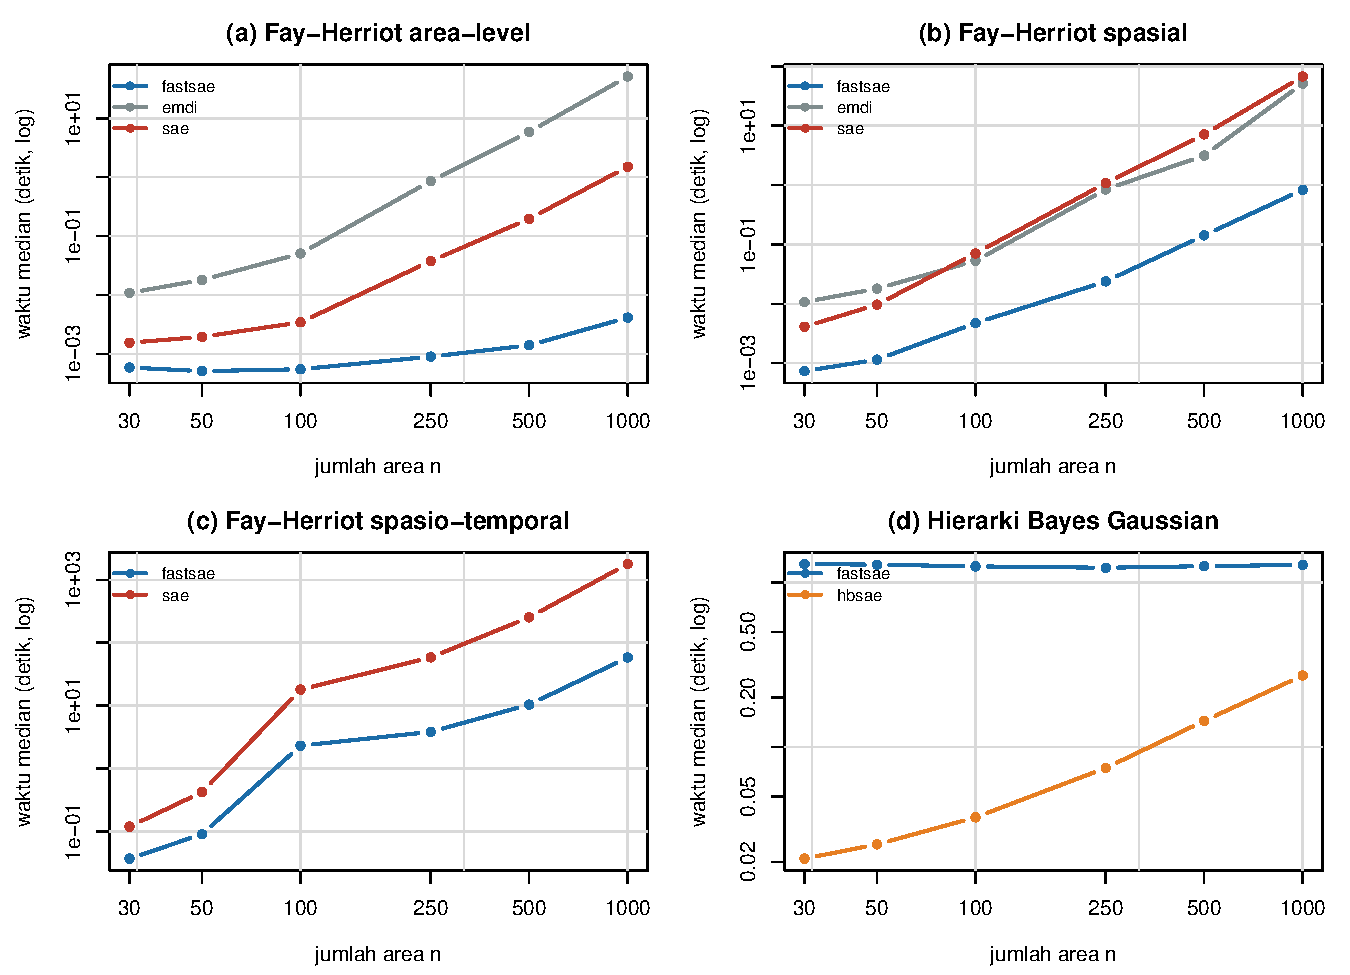
\includegraphics[width=\textwidth]{fig-time-fh.pdf}
  \caption{Waktu median per iterasi terhadap jumlah area $n$ (skala log pada
  kedua sumbu). Sumber: \texttt{inst/extdata/eblup\_benchmark.rds},
  \texttt{seblup\_benchmark.rds}, \texttt{steblup\_benchmark.rds},
  \texttt{hb\_benchmark.rds}; digambar oleh \texttt{scripts/02\_figures.R}.}
  \label{fig:time-fh}
\end{figure}

\begin{figure}[htbp]
  \centering
  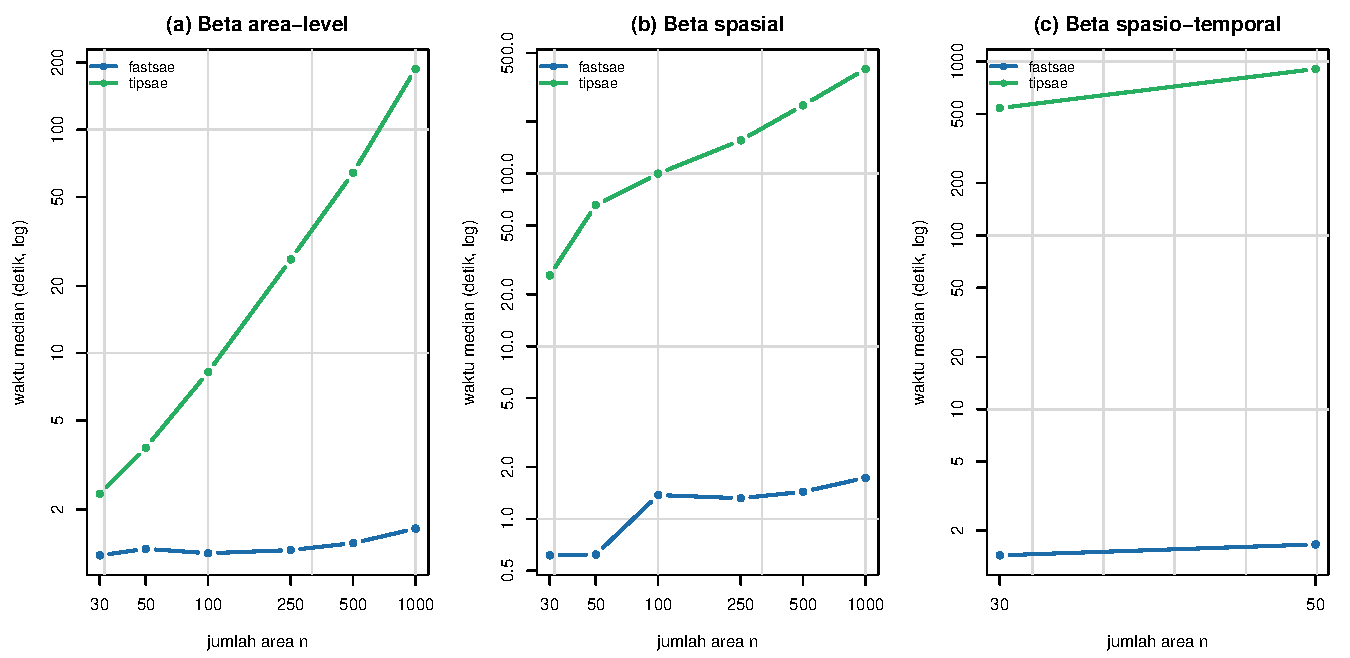
\includegraphics[width=\textwidth]{fig-time-beta.pdf}
  \caption{Waktu median untuk tiga varian model beta (skala log--log).
  Sumber: \texttt{inst/extdata/beta\_benchmark.rds},
  \texttt{spatial\_beta\_benchmark.rds},
  \texttt{spatio\_temporal\_beta\_benchmark.rds}; \texttt{scripts/02\_figures.R}.
  Panel (c) hanya memiliki $n=30$ dan $n=50$.}
  \label{fig:time-beta}
\end{figure}

\begin{figure}[htbp]
  \centering
  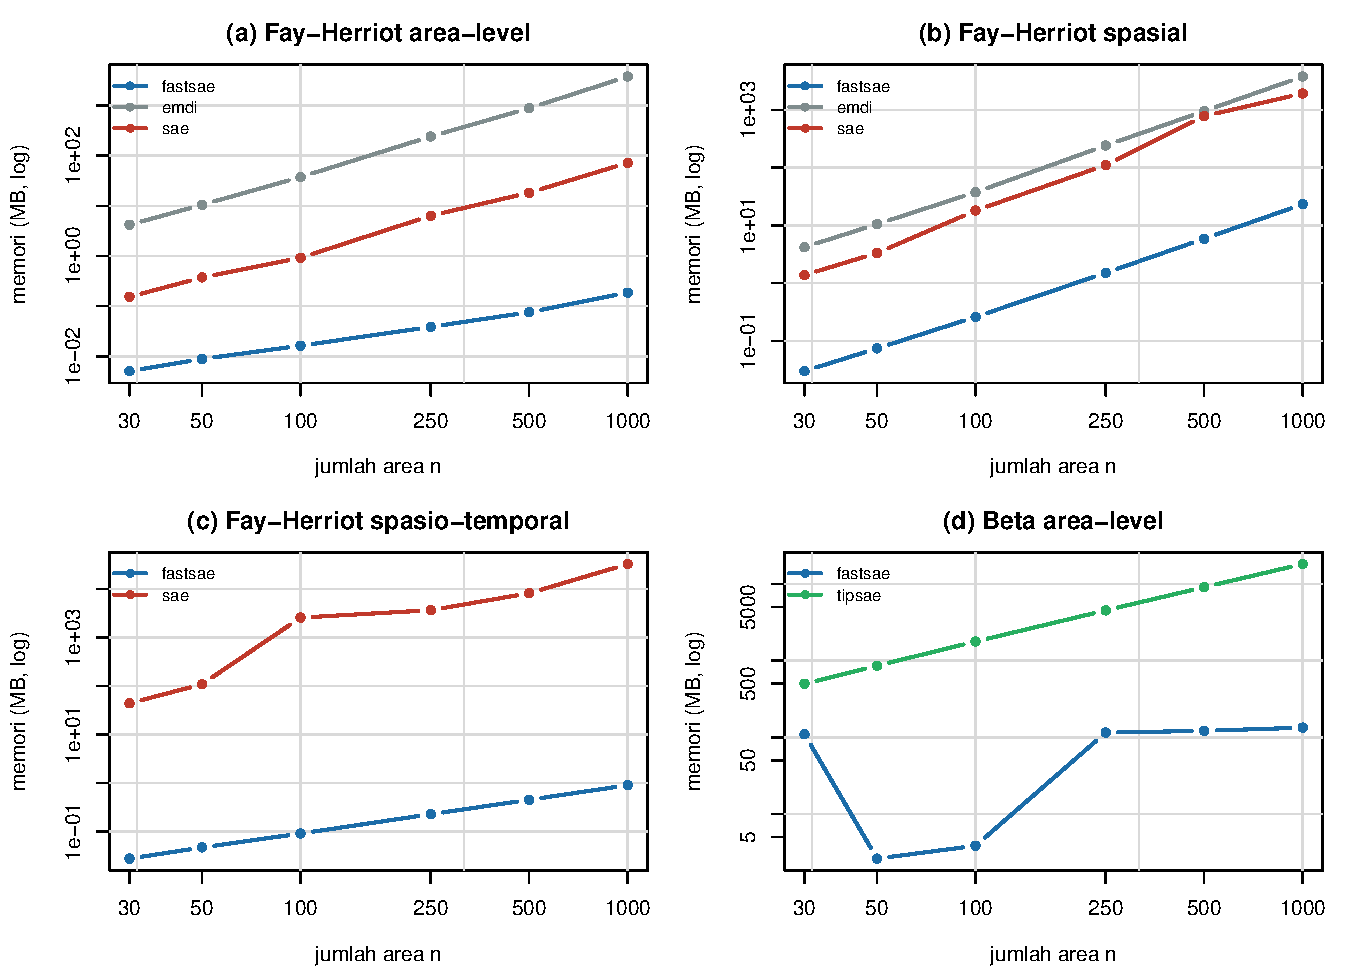
\includegraphics[width=\textwidth]{fig-mem.pdf}
  \caption{Alokasi memori total per iterasi terhadap $n$ (skala log--log).
  Sumber: file \texttt{inst/extdata/*\_benchmark.rds} sebagaimana tercantum pada
  tiap panel; \texttt{scripts/02\_figures.R}.}
  \label{fig:mem}
\end{figure}

\begin{figure}[htbp]
  \centering
  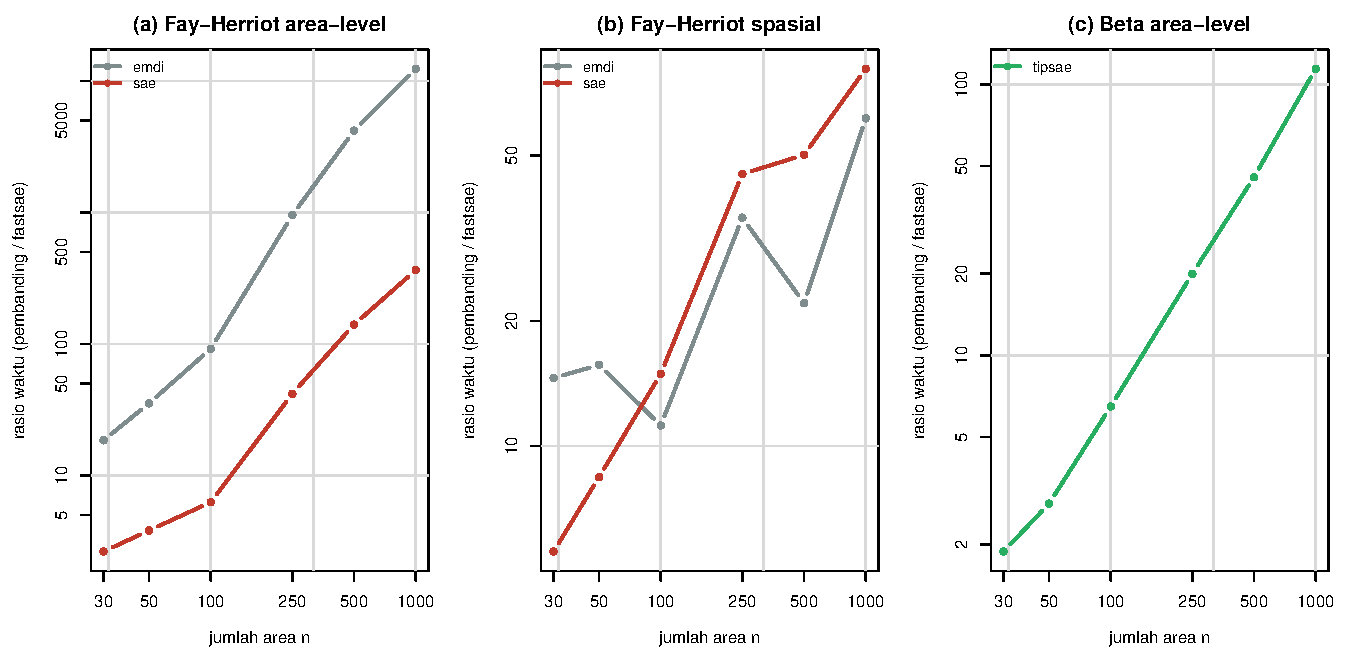
\includegraphics[width=\textwidth]{fig-ratio.pdf}
  \caption{Rasio waktu (pembanding/tes) terhadap $n$; garis putus-putus
  menandai rasio $=1$. Sumber: file \texttt{inst/extdata/*\_benchmark.rds};
  \texttt{scripts/02\_figures.R}.}
  \label{fig:ratio}
\end{figure}

Tabel~\ref{tab:ratio} merangkum seluruh rasio per $n$. Rentangnya
jauh lebih lebar daripada klaim di \code{README.Rmd}: pada ujung bawah ada
skenario tempat pembanding lebih cepat dari \pkg{fastsae}, dan pada ujung
atas rasio mencapai empat orde magnitudo --- karenanya laporan memilih
menampilkan rentang, bukan satu angka tunggal.

\begin{table}[htbp]
\centering
\caption{Rasio kecepatan $=$ median waktu pembanding $/$ median waktu \texttt{fastsae} (semakin besar semakin cepat \texttt{fastsae}; nilai $<1$ berarti pembanding lebih cepat). Rasio dihitung per $n$ lalu diringkas.}
\label{tab:ratio}
\small
\begin{tabular}{llrrrr}
\toprule
Model & Pembanding & $n$ pertama & $n$ terbesar & min & max \\
\midrule
FH area-level (\texttt{eblup\_fh}) & emdi & 18.5018 & 12343.4 & 18.5018 & 12343.4 \\
 & \multicolumn{5}{r}{\emph{rata-rata lintas $n$: 2936.41$\times$}} \\[-2pt]
FH area-level (\texttt{eblup\_fh}) & sae &  2.6386 &  363.76 &  2.6386 &  363.76 \\
 & \multicolumn{5}{r}{\emph{rata-rata lintas $n$: 93.0598$\times$}} \\[-2pt]
FH spasial (\texttt{eblup\_sfh}) & emdi & 14.5797 & 61.3577 &  11.213 & 61.3577 \\
 & \multicolumn{5}{r}{\emph{rata-rata lintas $n$: 26.7192$\times$}} \\[-2pt]
FH spasial (\texttt{eblup\_sfh}) & sae & 5.58264 &  80.696 & 5.58264 &  80.696 \\
 & \multicolumn{5}{r}{\emph{rata-rata lintas $n$: 34.1403$\times$}} \\[-2pt]
FH spasio-temporal (\texttt{eblup\_stfh}) & sae & 3.22733 & 30.7484 & 3.22733 & 30.7484 \\
 & \multicolumn{5}{r}{\emph{rata-rata lintas $n$:   14.37$\times$}} \\[-2pt]
Beta area-level (\texttt{hb\_area}) & tipsae & 1.88664 & 114.146 & 1.88664 & 114.146 \\
 & \multicolumn{5}{r}{\emph{rata-rata lintas $n$: 31.7991$\times$}} \\[-2pt]
Beta spasial & tipsae &  41.906 & 233.978 &  41.906 & 233.978 \\
 & \multicolumn{5}{r}{\emph{rata-rata lintas $n$: 124.435$\times$}} \\[-2pt]
Beta spasio-temporal & tipsae & 374.863 & 544.576 & 374.863 & 544.576 \\
 & \multicolumn{5}{r}{\emph{rata-rata lintas $n$:  459.72$\times$}} \\[-2pt]
Hierarki Bayes Gaussian & hbsae & 0.0162013 & 0.212725 & 0.0162013 & 0.212725 \\
 & \multicolumn{5}{r}{\emph{rata-rata lintas $n$: 0.0756733$\times$}} \\[-2pt]
\bottomrule
\end{tabular}
\end{table}



\subsection{Ekuivalensi numerik terhadap pembanding}\label{sec:ekuivalensi}

File \code{beta\_estimates\_n1000.rds} memuat pasangan estimasi dan MSE untuk
1000 area antara \pkg{fastsae} dan \pkg{tipsae} pada model beta yang sama.
Tabel~\ref{tab:equiv} menghitung metrik kesesuaian dari pasangan kolom itu;
Gambar~\ref{fig:equiv} menampilkannya secara grafis.

\begin{table}[htbp]
\centering
\caption{Ekuivalensi numerik antara \texttt{fastsae} dan \texttt{tipsae} pada $n=1000$ area (indikator beta). Semua metrik dihitung dari pasangan kolom pada file sumber.}
\label{tab:equiv}
\small
\begin{tabular}{lr}
\toprule
Metrik & Nilai \\
\midrule
Pearson $r$ (estimasi) & 0.999343 \\
Spearman $\rho$ (estimasi) & 0.999208 \\
MAE (estimasi) & 0.0196916 \\
RMSD (estimasi) & 0.0236901 \\
Galat absolut maksimum & 0.0558335 \\
Pearson $r$ (MSE) & 0.963148 \\
Median selisih mutlak MSE & 0.000171686 \\
Median rasio MSE fastsae/tipsae & 2.21687 \\
\bottomrule
\end{tabular}
\end{table}



\begin{figure}[htbp]
  \centering
  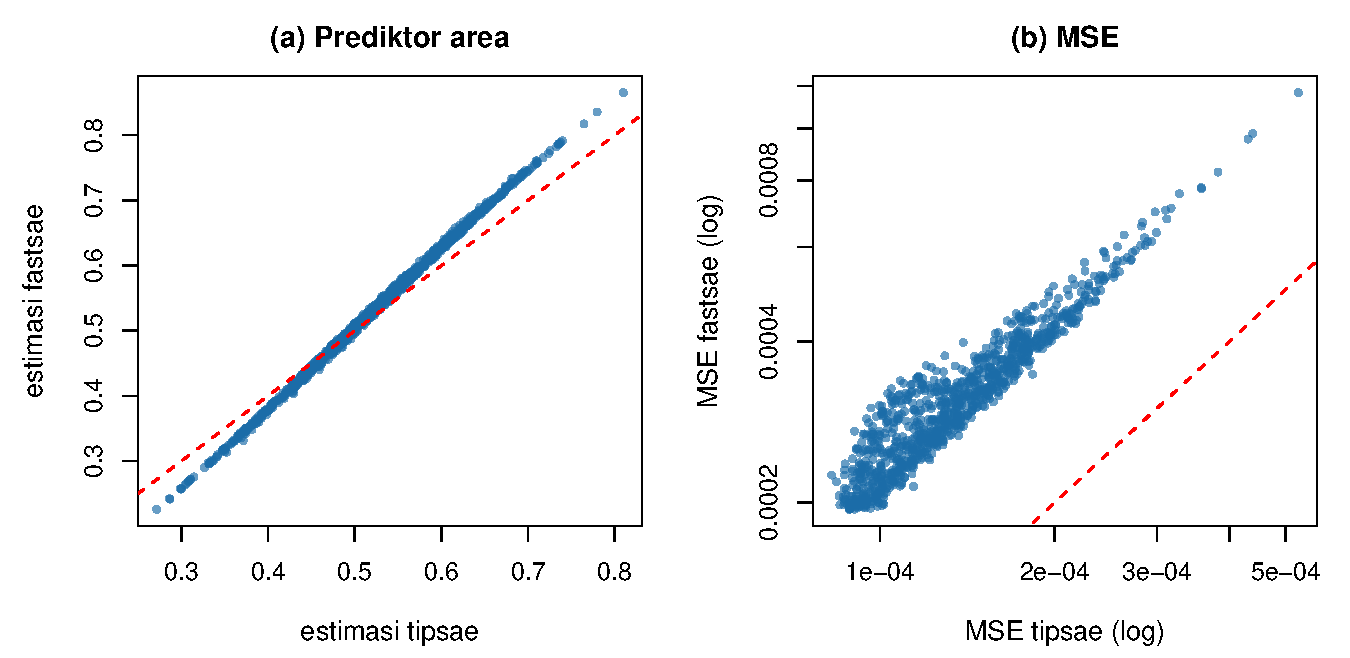
\includegraphics[width=\textwidth]{fig-equiv.pdf}
  \caption{Ekuivalensi numerik \texttt{fastsae} vs \texttt{tipsae} untuk
  $n=1000$ area: (a) prediktor area terhadap garis identitas;
  (b) MSE pada skala log. Sumber: \texttt{inst/extdata/beta\_estimates\_n1000.rds};
  \texttt{scripts/02\_figures.R}.}
  \label{fig:equiv}
\end{figure}

Kedua paket memprediksi indikator yang sama dengan selisih kecil pada prediktor
(korelasi sangat tinggi; Tabel~\ref{tab:equiv}), sedangkan MSE berbeda lebih
nyata karena kedua paket memakai pendekatan ketidakpastian yang berbeda (INLA
Laplace vs posterior MCMC). Angka MSE tidak boleh dibaca sebagai ``satu paket
lebih benar'' tanpa rujukan kebenaran; pembanding terhadap kebenaran model
tersedia pada skrip \code{benchmarks/compare\_ebp\_tipsae\_truth.R} dan
\code{sim\_mc\_finite\_population.R} (hasil tersimpan di
\code{benchmarks/output/}, di luar cakupan \code{inst/extdata}).

\subsection{Kaveat dan keadilan}\label{sec:kaveat}

\begin{enumerate}[label=\arabic*.]
  \item \textbf{Beda algoritme, bukan beda implementasi.} \pkg{tipsae} adalah
        Bayes MCMC/Stan \citep{denicolo2024tipsae}, \pkg{hbsae} memakai
        pendekatan Bayesnya sendiri, \pkg{emdi} dan \pkg{sae} memakai
        \pkg{lme4}/aljabar \pkg{Matrix} di R, sedangkan \pkg{fastsae} memakai
        C++ + INLA. Selisih waktu mencerminkan perbedaan ini sekaligus.
  \item \textbf{Tanpa penetapan thread.} Tidak ada skrip yang mengunci
        \code{OMP\_NUM\_THREADS}; bootstrap paralel (bagian
        \ref{sec:bootstrap-paralel}) dapat memakai seluruh core mesin,
        sedangkan pembanding berjalan serial. Ini membuat perbandingan
        \emph{memihak} ke \pkg{fastsae} pada skala besar, dan dilaporkan apa
        adanya.
  \item \textbf{Kriteria konvergensi tidak disamakan.} \pkg{fastsae} memakai
        toleransi $10^{-4}$ dan 100 iterasi (Tabel~\ref{tab:konvergensi});
        pengaturan pembanding tidak tercatat di file.
  \item \textbf{Memori bukan puncak.} Kolom memori adalah akumulasi alokasi,
        sehingga tidak setara dengan \emph{peak RSS} yang lazim dilaporkan.
  \item \textbf{Empat file tanpa skrip.} Hasil FH (tiga file) dan
        \code{beta\_estimates\_n1000} tidak dapat direproduksi dari repo;
        laporan memakainya apa adanya dan menandainya.
  \item \textbf{Run inkremental.} Skrip 1--5 menulis file secara inkremental
        (baris lama per $n$ diganti), sehingga file bisa berisi campuran run
        dari waktu yang berbeda.
\end{enumerate}

\subsection{Kontradiksi klaim dokumentasi terhadap data}\label{sec:kontradiksi}

Aturan laporan: data menang. Temuan berikut berasal dari perbandingan langsung
klaim \code{README.Rmd}/\code{vignettes/benchmarks.Rmd}/\code{paper/article.tex}
dengan isi \code{inst/extdata} (perhitungan lengkap:
\code{\_notes/bench\_methodology.md} bagian 6 dan 8).

\begin{table}[htbp]
\centering
\caption{Klaim dokumentasi yang bertolak belakang dengan file data. Sumber:
\texttt{README.Rmd}, \texttt{vignettes/benchmarks.Rmd}, \texttt{paper/article.tex}
vs \texttt{inst/extdata/*.rds} (butir DOC-1\,--\,DOC-11 di \texttt{DISCREPANCIES.md}).}
\label{tab:kontradiksi}
\small
\begin{tabularx}{\textwidth}{@{}l X X@{}}
\toprule
Butir & Klaim dokumentasi & Fakta dari data \\
\midrule
DOC-1 & \code{README.Rmd:118} menandai tabel ``Benchmark across $n=1000$
  areas'' & angka tabel adalah rata-rata lintas $n=30\ldots1000$ \\
DOC-2 & \code{README.Rmd:122} ``$\sim$190$\times$'' dan ``$\sim$6400$\times$'' &
  rasio yang benar tidak cocok dengan salah satunya (lihat Tabel~\ref{tab:ratio}) \\
DOC-3 & \code{README.Rmd:124} fastsae ``$<$ 10 MB'' &
  beberapa baris \pkg{fastsae} melebihi 10 MB (Tabel~\ref{tab:mem-summary}) \\
DOC-4 & \code{README.Rmd:124} pembanding ``$\sim$400 MB''/``$\sim$800 MB'' &
  campuran dua file; untuk FH angkanya jauh di bawah itu \\
DOC-5/6 & \code{README.Rmd:34-35} ``50 to 6{,}000$\times$'' dan
  \code{:87} ``10--100$\times$'' &
  rentang teramati lebih lebar di kedua ujung (Tabel~\ref{tab:ratio}) \\
DOC-7 & \code{vignettes/benchmarks.Rmd:39} emdi spasial ``8{,}69 s'' &
  nilai pada file berbeda (Tabel~\ref{tab:time-sfh}) \\
DOC-8 & label ``\emph{Peak} Memory'' di README, vignette, dan artikel &
  nilai adalah rerata \code{mem\_alloc}, bukan puncak \\
DOC-9 & \code{paper/article.tex:100,480} ``73$\times$ to 544$\times$'' &
  ada nilai serendah $1{,}887\times$ (Tabel~\ref{tab:ratio}) \\
DOC-10 & \code{vignettes/}\allowbreak{}\code{benchmarks.Rmd:407-414,}\allowbreak{}\code{634-639} kolom Spatial/ST
  $n\ge100$ & tidak ada data pendukung di \code{inst/extdata} \\
DOC-11 & reproduksi hasil & empat file tidak punya skrip pembuat di repo \\
\bottomrule
\end{tabularx}
\end{table}

Implikasinya langsung: laporan ini tidak mengutip satu pun angka kecepatan
dari README. Angka yang dipakai seluruhnya berasal dari tabel dan gambar di
atas, yang kesemuanya dihasilkan ulang dari file data.

% ===========================================================================
%  Bagian 4 -- Latar statistik
% ===========================================================================
\section{Latar statistik}\label{sec:latar}

Bagian ini menyajikan perkakas yang dipakai berulang di seluruh model, dengan
notasi yang sama dengan yang dipakai kode (mis.\ nama variabel
\code{vardir}, \code{sigma2}, \code{rho}). Derivasi panjang dipindahkan ke
lampiran~\ref{sec:derivasi}.

\subsection{Tabel notasi}\label{sec:notasi}

\begin{table}[htbp]
\centering
\caption{Notasi utama dan padanannya dalam kode. Sumber: simbol pada
\code{R/*.R} dan \code{src/*.cpp}.}
\label{tab:notasi}
\small
\begin{tabularx}{\textwidth}{@{}l l X@{}}
\toprule
Simbol & Nama kode & Arti \\
\midrule
$y_d$ atau $y_{id}$ & \code{y} & pengamatan langsung / respons (baris \code{NA}
  menandai domain tak-sampel pada model area-level) \\
$\psi_d$ & \code{vardir}, \code{psi} & varian pengukuran langsung
  $\psi_d=S_d^2/n_d$; wajib $>0$ pada area tersampel \\
$\Xmat$ & \code{X}, \code{Xall} & matriks desain ($m\times p$ atau $N\times p$) \\
$\betah$ & \code{beta} & estimasi koefisien fit tetap (GLS) \\
$u_d$, $\theta_d$ & \code{random\_effect}, \code{theta} & efek acak domain dan
  prediktor area $\theta_d=x_d'\beta+u_d$ \\
$\sigma^2$ & \code{sigma2}, \code{sigma2\_u} & varians efek acak \\
$\Vm$ & \code{V}, \code{Vi} & kovarians respons dan inversinya \\
$\Qm=(\Xmat'\Vm^{-1}\Xmat)^{-1}$ & \code{Q} & matriks informasi GLS \\
$w_d=1/(\psi_d+\sigma^2)$ & \code{w} & bobot FH per area \\
$B_d$ & \code{Bd} & faktor pemulusan gaya FH (lihat \eqref{eq:g1g2g3}) \\
$h_d=x_d'\Qm x_d$ & \code{h} & leverage prediktor \\
$\Wmat$ & \code{W}, \code{proxmat} & matriks tetangga (bobot) \\
$\rho$ & \code{rho} & autoregresi spasial pada SFH/STFH \\
$f_d=n_d/N_d$ & \code{f} & fraksi sampel populasi (BHF, \code{hb\_unit}) \\
$B$ & \code{B} & jumlah replikat bootstrap \\
$m$, $M$, $D$, $T$ & \code{m}, \code{D}, \texttt{Tt} & jumlah area ter-sampel,
  total baris, jumlah domain, jumlah periode waktu \\
\bottomrule
\end{tabularx}
\end{table}

\subsection{Model campuran linear, GLS, dan BLUP}\label{sec:lmm}

Model campuran linear umum
\begin{equation}
  y=\Xmat\beta+\Zmat u+\varepsilon,\qquad
  \begin{pmatrix}u\\\varepsilon\end{pmatrix}
  \sim N\!\left(0,\;
  \begin{pmatrix}\mathbf G&0\\0&\Rmat\end{pmatrix}\right),
  \label{eq:lmm}
\end{equation}
memberi kovarians total $\Vm=\Zmat\mathbf G\Zmat'+\Rmat$. Dengan $\beta$
diketahui, prediktor linier tak bias terbaik (BLUP) dari $u$ adalah
\begin{equation}
  \tilde u=\mathbf G\Zmat'\Vm^{-1}(y-\Xmat\beta),
  \qquad
  \tilde\theta=\Xmat\beta+\mathbf G\Zmat'\Vm^{-1}(y-\Xmat\beta).
  \label{eq:blup}
\end{equation}
Apabila $\beta$ dinilai dengan GLS, $\betah=(\Xmat'\Vm^{-1}\Xmat)^{-1}
\Xmat'\Vm^{-1}y$, maka prediktor \eqref{eq:blup} tetap linier tak bias pada
$\beta$ dan dikenal sebagai \emph{best linear unbiased predictor}
\citep{kackar1984approximations}. Pada \pkg{fastsae}, \eqref{eq:blup} muncul
sebagai \code{eblup = Xbeta + GVi \%*\% (y - Xbeta)} pada SFH
(\code{eblup\_sfh\_core.cpp:462}) dan sebagai kasus khusus pada FH.

Untuk model area-level FH, $\Zmat=\Imat$, $\mathbf G=\sigma^2\Imat$,
$\Rmat=\mathrm{diag}(\psi_d)$ sehingga $\Vm$ diagonal dan semua operasi
turun ke skalar per area:
\begin{equation}
  \hat u_d=\frac{\sigma^2}{\sigma^2+\psi_d}\,(y_d-x_d'\betah),
  \qquad
  \hat\theta_d=x_d'\betah+\hat u_d.
  \label{eq:fh-blup}
\end{equation}

\subsection{EBLUP}\label{sec:eblup}

\emph{Empirical} BLUP menggantikan komponen varians $\sigma^2$ dengan
estimanya $\hat\sigma^2$:
\begin{equation}
  \hat\theta_d(\hat\sigma^2)=x_d'\betah(\hat\sigma^2)
  +\hat u_d(\hat\sigma^2).
  \label{eq:eblup}
\end{equation}
\citet{kackar1984approximations} menunjukkan bahwa pendekatan orde-kedua
menyediakan pendekatan varian prediktor yang lazim dipakai; \citet{prasad1990estimation}
dan \citet{datta2000unified} mengembangkan dekomposisinya menjadi suku-suku
$g$ yang dibahas pada bagian~\ref{sec:mse}. Konsekuensi praktis pendekatan ini
diabaikan oleh Kackar--Harville: penggantian $\sigma^2\to\hat\sigma^2$
menggeser prediktor sedikit ke atas (\emph{bias}); pada FH, \pkg{fastsae}
mengoreksi orde-kedua itu \emph{hanya} bila \code{method = "ML"}
(\code{eblup\_fh.cpp:196-199}).

\subsection{ML, REML, dan skor}\label{sec:ml-reml}

Likelihood biasa untuk FH (satu parametrik) dengan
$v_d=\sigma^2+\psi_d$:
\begin{equation}
  \ell(\sigma^2)=-\frac12\sum_{d=1}^{m}
  \left[\log(2\pi v_d)+\frac{r_d^2}{v_d}\right],
  \qquad r_d=y_d-x_d'\betah,
  \label{eq:loglik-ml}
\end{equation}
dengan $\betah$ fungsi GLS dari $\sigma^2$. Persamaan skor ML yang
dikodekan (\code{eblup\_fh.cpp:103}) adalah
\begin{equation}
  s(\sigma^2)=-\frac12\sum_d w_d+\frac12(Py)'(Py),
  \qquad P=W-WX\Qm X'W,
  \label{eq:score-fh-ml}
\end{equation}
dan informasi Fisher $I(\sigma^2)=\frac12\sum_d w_d^2$
(\code{eblup\_fh.cpp:112}). REML memakai kasus spesial
\begin{equation}
  s_R(\sigma^2)=-\frac12\tr P+\frac12(Py)'(Py),
  \qquad I_R(\sigma^2)=\tfrac12\tr(P^2),
  \label{eq:score-fh-reml}
\end{equation}
dengan turunan ringkas yang dikodekan: $\tr P=\sum_d w_d-\tr(\Qm
\Xmat'W^2\Xmat)$ dan $\tr(P^2)=\sum w^2-2\sum_d w_d^2(x_d'\Qm x_d)w_d
+\tr(K^2)$, $K=\Qm\Xmat'W^2\Xmat$ (\code{eblup\_fh.cpp:105-117}).
Tidak ada inversi matriks $m\times m$ sama sekali pada FH: kedua turunan
dihitung dari akumulasi skalar.

\begin{implnote}
Untuk model dengan dua atau lebih parameter (dua-fold, SFH, STFH),
persamaan skor ditulis per elemen $\theta_a$ dengan pola
$s_a=-\tfrac12\tr(M_a)+\tfrac12 y'M_a y$ (REML) dan
$\mathcal I_{ab}=\tfrac12\tr(M_aM_b)$, dengan $M_a=P\,\partial V/\partial
\theta_a$ dan $P=V^{-1}-V^{-1}X\Qm X'V^{-1}$. Untuk SFH dengan
\code{method="ML"}, kode memakai kuadratik $y'PDPy$ tetapi informasi
$\tfrac12\tr(V^{-1}D_aV^{-1}D_b)$ --- campuran ML/REML yang didokumentasikan
sebagai SFH-1 di \code{DISCREPANCIES.md}.
\end{implnote}

\subsection{Fisher scoring}\label{sec:fs}

Fisher scoring menggantikan Hessian oleh informasi Fisher:
\begin{equation}
  \theta^{(k+1)}=\theta^{(k)}+\mathcal I(\theta^{(k)})^{-1}
  s(\theta^{(k)}).
  \label{eq:fisher}
\end{equation}
Algoritme umum yang diikuti empat inti C++ (lihat
Tabel~\ref{tab:konvergensi} untuk nilai konkretnya):
\begin{enumerate}[label=\arabic*.]
  \item hitung $\Vm,\Vm^{-1},\Qm$ pada $\theta^{(k)}$;
  \item hitung skor $s$ dan informasi $\mathcal I$;
  \item langkah $\Delta=\mathcal I^{-1}s$ (pada dua-parameter: inversi
        $2\times2$; bila gagal, fallback $\Delta_a=s_a/\mathcal I_{aa}$);
  \item perbarui $\theta\leftarrow\theta+\Delta$; terapkan batas;
  \item uji $\texttt{diff}=\max_a\abs{\Delta_a/\max(\theta_a,10^{-12})}\le
        \texttt{precision}$;
  \item ulangi maksimum \code{maxiter} kali, lalu lakukan pass akhir pada
        $\hat\theta$ (menghitung ulang $\Qm,\betah$, galat baku, prediktor,
        dan MSE).
\end{enumerate}
Langkah 6 penting: MSE dan galat baku dievaluasi pada $\hat\theta$ final,
bukan pada iterate terakhir sebelum update (pada STFH, galat baku parameter
komponen varians justru dihitung dari $\mathcal I^{-1}$ pada $\theta_k$
sebelum update terakhir --- STFH-7 di \code{DISCREPANCIES.md}).

\subsection{Dekomposisi MSE}\label{sec:mse}

Untuk prediktor EBLUP, \citet{prasad1990estimation} dan
\citet{kackar1984approximations} menguraikan galat kuadrat rata-rata ke dalam
tiga suku. Untuk FH, \pkg{fastsae} menghitung (\code{eblup\_fh.cpp:183-202})
dengan parametrisasi
\begin{equation}
  B_d=\frac{\psi_d}{\psi_d+\sighat},
  \qquad
  g_1=\psi_d(1-B_d),
  \qquad
  g_2=B_d^2\,h_d,
  \qquad
  g_3=B_d^2\,\frac{\VarA}{\sighat+\psi_d},
  \label{eq:g1g2g3}
\end{equation}
dengan $\VarA=2/\sum_d w_d^2$ (varian asimptotik $\hat\sigma^2$), $h_d=x_d'
\Qm x_d$. Lalu
\begin{equation}
  \widehat{\mathrm{MSE}}(\hat\theta_d)=
  \begin{cases}
    g_1+g_2+2g_3, & \text{REML},\\[2pt]
    g_1+g_2+2g_3-b\,B_d^2, & \text{ML},
  \end{cases}
  \qquad
  b=-\frac{\tr(\Qm\Xmat'W^2\Xmat)}{\max\bigl(\sum_d w_d^2,10^{-30}\bigr)}.
  \label{eq:mse-fh}
\end{equation}
\implnote{$B_d$ pada \eqref{eq:g1g2g3} adalah komplemen dari
$B_d=\sighat/(\sighat+\psi_d)$ yang lazim dipakai Rao--Molina: kode menulis
$B_d=\psi_d/(\psi_d+\sighat)$ (FH-1). Bentuk $g_1=\psi_d(1-B_d)$ ekuatip dengan
$(B_d^{\text{RM}})^2\psi_d+(1-B_d^{\text{RM}})^2\sighat$ (FH-2). Jangan tertukar
dengan $(1-B)^2(\psi_d+\sighat)$ yang kadang muncul di literatur --- bentuk itu
bukan yang dikodekan.}

Untuk model dua-parameter (dua-fold) koreksi bias berbeda: varians
$\Var(\hat\sigma_v^2)$, $\Var(\hat\sigma_u^2)$, dan $\Cov$ diambil dari
invers matriks informasi Fisher final, dan
$\mathrm{MSE}=g_1+g_2+g_3$ dengan suku silang $2\E_{vu}\Cov_{vu}$ sudah
termasuk di dalam $g_3$ (TFH-2) --- bukan $g_1+g_2+2g_3$. Untuk SFH, empat
suku dipakai: $\mathrm{MSE}=g_1+g_2+2g_3-g_4$ plus koreksi bias ML pada
$g_1$ (bagian~\ref{sec:sfh-mse}).

\subsection{MSE bootstrap}\label{sec:bootstrap}

Dua jenis tersedia di paket:

\paragraph{Parametrik.} Dari hasil fit $\hat\beta,\hat\sigma^2$, bangkitkan
$y^\ast=\Xmat\hat\beta+u^\ast+\varepsilon^\ast$ dengan $u^\ast,\varepsilon^\ast$
dari distribusi model, refit, lalu
\begin{equation}
  \widehat{\mathrm{MSE}}_{\mathrm{pb}}
  =\frac1B\sum_{b=1}^B\bigl(\hat\theta_b^\ast-\theta_b^\ast\bigr)^2.
  \label{eq:pbmse}
\end{equation}
Ini persis \code{eblup\_twofold.cpp:515-517}, \code{eblup\_stfh\_pbmse.cpp:405-412},
\code{eblup\_sfh\_pbmse.cpp:158-164}, dan \code{R/eblup\_bhf.R:360}. Varian
bias-koreksi pada SFH memakai
\begin{equation}
  \widehat{\mathrm{MSE}}_{\mathrm{pbbc}}
  =2(g_1+g_2)-g_1^\ast-g_2^\ast+g_3^\ast,
  \label{eq:pbbc}
\end{equation}
dengan $g_3^\ast$ diambil dari selisih $\hat\theta^\ast$ terhadap prediksi
SBLUP yang bobotnya berasal dari \emph{fit awal}
(\code{eblup\_sfh\_pbmse.cpp:127-128,164}); kesesuaian \eqref{eq:pbbc}
dengan rumus publik tidak terikat pada referensi mana pun di repo dan
ditandai tidak pasti (SFH-10).

\paragraph{Nonparametrik.} Hanya untuk SFH dan hanya REML
(\code{eblup\_sfh\_npbmse.cpp:32-34}): residual dibagi menjadi komponen
efek acak dan sampling lewat akar kuadrat matriks $\Psi_e=\mathrm{diag}(\psi)
P\,\mathrm{diag}(\psi)$ dan $\Psi_u=(\Imat-\rho W)\,G\,P\,G(\Imat-\rho W)'$
yang dieigendekomposisi (kolom $p..m-1$ dipakai untuk membuang arah proyeksi
$\Xmat$), lalu resample indeks residual yang telah distandarisasi
(\code{eblup\_sfh\_npbmse.cpp:70-110,143-149}).

\subsection{Domain tanpa sampel dan prediksi sintetis}\label{sec:unsampled}

Tabel~\ref{tab:unsampled} merangkum perilaku tiap fungsi terhadap domain tanpa
pengamatan. Definisi ``tanpa sampel'' berbeda antar fungsi, dan perbedaan itu
penting bagi pengguna.

\begin{table}[htbp]
\centering
\caption{Penanganan domain tanpa sampel. Sumber: cabang kode pada kolom terakhir.}
\label{tab:unsampled}
\small
\begin{tabularx}{\textwidth}{@{}l l X@{}}
\toprule
Fungsi & Kriteria & Prediktor dan MSE \\
\midrule
\code{eblup\_fh} & \code{y = NA} & $x_{ns}'\betah$;
  $\mathrm{MSE}=\sighat+x_{ns}'\Qm x_{ns}$; \code{random\_effect = NA}
  (\code{eblup\_fh.cpp:207-222}) \\
\code{eblup\_sfh} & \code{y = NA} & kriging $x_{ns}'\betah+G_{rs}\Vm^{-1}r$
  dengan sub-blok $A_{full}^{-1}$; $\mathrm{MSE}=g_1+g_2$ saja
  (\code{eblup\_sfh\_core.cpp:576-604}) \\
\code{eblup\_stfh} & respons \code{NA} & \emph{tidak diizinkan}: panel wajib
  lengkap, \code{cli\_abort} (\code{R/eblup\_stfh.R:129-139}) \\
\code{eblup\_bhf} & domain tanpa unit sampel & prediktor sintetis
  $\bar x_{pop}'\betah$, \code{samp\_size = 0}, peringatan
  (\code{eblup\_unit.cpp:94-100}) \\
\code{eblup\_twofold} & \code{y = NA} & area tanpa subarea: $x'\betah$;
  subarea tak-sampel pada area tersampel: $x'\betah+\hat v_i$
  (\code{eblup\_twofold.cpp:333-363}) \\
\code{hb\_unit} & seluruh domain & menambahkan 1 baris \code{y = NA} per
  domain, lalu memakai fitted INLA (\code{hb\_unit.R:244-249}) \\
\code{hb\_area}, \code{hb\_twofold} & baris \code{y = NA} & tetap dievaluasi
  oleh INLA; domain yang \emph{tidak ada dalam data} tidak diprediksi
  (HB-17) \\
\bottomrule
\end{tabularx}
\end{table}

\subsection{Benchmarking: pengertian internal dan eksternal}\label{sec:bench-def}

Dalam literatur SAE, \emph{benchmarking} berarti mengkalibrasi prediktor
model ke total atau agregat yang diketahui sehingga konsistensi antar tingkat
kerapian terpenuhi \citep{rao2015small}. Dua varian muncul di paket ini:

\begin{itemize}
  \item \textbf{Benchmarking eksternal} memakai total populasi yang diketahui
        dari sumber luar survei (mis.\ total penduduk per provinsi).
  \item \textbf{Benchmarking internal} menggunakannya sebagai \emph{validasi}:
        \code{diagnose()} membandingkan total prediksi terhadap total yang
        diketahui dan menandai status \code{CONSISTENT} bila selisihnya di
        bawah toleransi (\code{benchmark.R:602}).
\end{itemize}

Empat metode kalibrasi (\code{ratio}, \code{difference}, \code{optimal},
\code{logit}) beserta pendukung hierarkinya dijelaskan pada
bagian~\ref{sec:utilitas}; di sini cukup dicatat bahwa seluruhnya bekerja pada
vektor prediktor + MSE dan bobot populasi, sehingga dapat dipakai pada hasil
model mana pun yang mengembalikan \code{df\_eblup}/\code{df\_hb}.

% ===========================================================================
%  Bagian 5.1 -- eblup_fh
% ===========================================================================
\section{Model Fay--Herriot area-level: \texttt{eblup\_fh}}\label{sec:fh}

\subsection{Setting data dan kapan dipakai}\label{sec:fh-setting}

Data berupa satu baris per domain: estimasi langsung $y_d$ (mis.\ rerata
tahun sekolah per kabupaten), varians pengukurannya $\psi_d$ (\code{vardir}),
dan kovariat $x_d$ berdimensi $p$ (jumlah sekolah, dll.). Model ini tepat
ketika: (i) survei menghasilkan estimasi langsung beserta variansnya, (ii)
domain sangat kecil sampai $y_d$ tidak stabil, dan (iii) ada kovariat yang
tersedia untuk semua domain termasuk yang tidak tersampel. Data contoh
\code{mys} (42 kabupaten, 10 di antaranya tanpa sampel) persis berbentuk ini.
Model ini adalah titik masuk klasik SAE \citep{fay1979small} dan dibahas
lengkap di \citet{rao2015small}.

\subsection{Persamaan model}\label{sec:fh-model}

\begin{equation}
  y_d=x_d'\beta+u_d+e_d,\qquad
  u_d\overset{\text{iid}}{\sim}N(0,\sigma^2),\qquad
  e_d\sim N(0,\psi_d),
  \label{eq:fh-model}
\end{equation}
dengan $\beta$ tanpa prior (dihilangkan lewat GLS) dan $e_d$ saling bebas.
Varians total per area $v_d=\sigma^2+\psi_d$ dan bobot
$w_d=1/v_d$ muncul di kode sebagai dasar seluruh turunan
(\code{eblup\_fh.cpp:89}). Dalam notasi blok, $\Vm=\diag(v_1,\dots,v_m)$.

Domain tanpa sampel ditandai \emph{bukan} lewat indeks melainkan lewat
\code{y = NA}: baris dengan \code{y} non-finite dipisahkan lebih dulu dan
$\Xmat$-nya disimpan sebagai \code{Xns} (\code{eblup\_fh.cpp:33-47}).
Argumen \code{domain} hanya pelabelan kolom (\code{R/eblup\_fh.R:97}).

\subsection{Prediktor titik}\label{sec:fh-prediktor}

Dengan $\betah=(\Xmat'W\Xmat)^{-1}\Xmat'Wy$ (\code{eblup\_fh.cpp:135-143}),
prediktor area adalah EBLUP
\begin{equation}
  \hat\theta_d=x_d'\betah+\hat u_d,\qquad
  \hat u_d=\frac{\sighat}{\sighat+\psi_d}\bigl(y_d-x_d'\betah\bigr),
  \label{eq:fh-pred}
\end{equation}
yang ekuivalen dengan pemulusan $y_d$ terhadap prediktor sintetis:
\begin{equation}
  \hat\theta_d=B_d\,(x_d'\betah)+(1-B_d)\,y_d,
  \qquad B_d=\frac{\psi_d}{\psi_d+\sighat}.
  \label{eq:fh-shrink}
\end{equation}
Pada domain tanpa sampel predikturnya jatuh ke prediktor sintetis murni
(\code{eblup\_fh.cpp:207-222}):
\begin{equation}
  \hat\theta_{ns}=x_{ns}'\betah,\qquad
  \widehat{\mathrm{MSE}}_{ns}=\sighat+x_{ns}'\Qm x_{ns},\qquad
  \texttt{random\_effect}=\texttt{NA}.
  \label{eq:fh-unsampled}
\end{equation}

\subsection{Estimasi komponen varians}\label{sec:fh-varians}

Algoritme Fisher scoring persis seperti bagian~\ref{sec:fs} dengan skor ML
\eqref{eq:score-fh-ml} dan skor REML \eqref{eq:score-fh-reml}. Rekam jejak
lengkapnya:

\begin{enumerate}[label=\arabic*.]
  \item \textbf{Nilai awal:} ${\sighat}{}^{(0)}=\max(\mathrm{median}(\psi_d),0)$
        (\code{eblup\_fh.cpp:64-65}).
  \item \textbf{Loop:} \code{while (diff > precision \&\& k < maxiter)}
        (\code{baris 88}), \code{precision} $=10^{-4}$, \code{maxiter} $=100$.
  \item \textbf{Per iterasi:} $W$, $\Qm=(\Xmat'W\Xmat)^{-1}$ lewat
        \code{inv\_sympd} dengan fallback \code{solve} (\code{baris 95-96}),
        $Py=Wy-\Xmat\Qm\Xmat'Wy$ (\code{baris 98-99}).
  \item \textbf{Update:} bila informasi $I\le0$ nilainya diganti
        \code{std::numeric\_limits<double>::min()} \emph{sebelum} dipakai
        membagi (\code{baris 120}), sehingga langkah menjadi raksasa lalu
        hasil non-finite atau negatif \emph{dipaksa} $0$ (\code{baris 121-123}).
  \item \textbf{Konvergensi:} $\texttt{diff}=\abs{({\sighat}{}^{\text{new}}-\sighat)/
        \max(\sighat,10^{-12})}$ (\code{baris 125}); status
        \code{convergence} dan \code{n\_iter} dikembalikan, dan wrapper R
        memperingati bila gagal (\code{R/eblup\_fh.R:104-107}).
  \item \textbf{Pass akhir:} hitung ulang $\Qm,\betah$, galat baku
        \code{se = sqrt(diag(Q))}, $z$, dan $p$ dua sisi pada $\sighat$ final
        (\code{baris 135-154}).
\end{enumerate}

Log-likelihood, AIC, dan BIC dihitung dari \eqref{eq:loglik-ml} dengan $m$
= jumlah area tersampel, $\mathrm{AIC}=-2\ell+2(p+1)$,
$\mathrm{BIC}=-2\ell+(p+1)\log m$ (\code{baris 170-174}).

\implnote{Ketiga ukuran kecocokan itu selalu berbentuk ML meski
\code{method = "REML"} (FH-3), dan koreksi bias orde-kedua
$-b\,B_d^2$ hanya dipakai untuk ML (FH-4) --- perilaku yang sama dengan
\pkg{sae::mseFH}. Kolom \code{estcoef} memuat dua kolom galat baku yang identik
(\code{std.error} dan \code{stderr\_beta}; FH-5), dan \code{vardir} wajib
positif ketat pada area tersampel (FH-6), yang tidak diperiksa \pkg{sae}.}

\subsection{Estimasi MSE}\label{sec:fh-mse}

MSE analitik \eqref{eq:mse-fh} adalah satu-satunya metode di \fct{eblup\_fh} --- tidak
ada pilihan bootstrap. RSE dilaporkan sebagai
$\mathrm{RSE}=100\sqrt{\mathrm{MSE}}/\abs{\hat\theta}$ dan menjadi
\code{NaN} bila $\hat\theta=0$ (\code{baris 227-230}). Pada domain tanpa
sampel dipakai \eqref{eq:fh-unsampled} tanpa suku $g_3$, sesuai
\citet{prasad1990estimation} untuk prediktor yang tidak memakai data domain.

\subsection{Pseudo-code}\label{sec:fh-algo}

\begin{algorithm}[htbp]
\caption{\texttt{eblup\_fh} --- alur sebenarnya (\texttt{R/eblup\_fh.R:49-113},
\texttt{src/eblup\_fh.cpp:9-264})}
\label{alg:fh}
\KwIn{formula, \code{vardir}, \code{domain}, \code{data},
  \code{method} $\in\{$REML, ML$\}$, \code{maxiter}, \code{precision}}
\KwOut{\code{df\_eblup} (prediktor, MSE, RSE), \code{estcoef}, \code{goodness}}
\SetKwFunction{FModelFrame}{model.frame}
\SetKwFunction{FCore}{eblup\_core}
\SetKwFunction{FPrint}{print}
\tcp*{\emph{Lapis R} --- \code{R/eblup\_fh.R}}
\code{method} $\leftarrow$ \texttt{match.arg}\tcp*{baris 59}
\code{domain} $\leftarrow$ \code{1:nrow(data)} bila \code{NULL} (60--64)\;
\code{mf} $\leftarrow$ \FModelFrame{formula, \code{na.action = na.pass}} (67)\;
\code{y} $\leftarrow$ respons, $\Xmat\leftarrow$ \texttt{model.matrix} (74--75)\;
\textbf{gagal} bila $\texttt{anyNA}(\Xmat)$ atau
$\texttt{length(vardir)}\ne\texttt{nrow(mf)}$ (70--80)\;
$\hat\theta,\widehat{\mathrm{MSE}},\ldots\leftarrow$ \FCore{$\Xmat,y,\psi$,
  \code{method}, \code{maxiter}, \code{precision}} (82)\;
sisipkan \code{domain} ke \code{df\_eblup}; \code{class} $\leftarrow$
\code{"fastsae"} (97--102)\;
\If{\texttt{!convergence}}{\texttt{cli\_alert\_danger} dan kembalikan (104--107)}
\FPrint{objek} bila \code{print\_result} (109--111)\;
\caption*{}
\SetKwFunction{FFindNonfinite}{find\_nonfinite}
\tcp*{\emph{Lapis C++} --- \code{src/eblup\_fh.cpp}}
$I_s\leftarrow$\FFindNonfinite{$y$}; $I_{ns}\leftarrow$\texttt{find\_finite}($y$)
  \tcp*{33--47}
\textbf{gagal} bila $m=0$ atau ada $\psi_d\le0$ pada area tersampel (53--59)\;
$\sighat\leftarrow\max(\mathrm{median}(\psi),0)$\;
$k\leftarrow0$;\quad $\texttt{diff}\leftarrow\texttt{precision}+1$\;
\While{\texttt{diff} $>$ \code{precision} \textbf{dan} $k<$ \code{maxiter}}{
  $W\leftarrow\diag(w)$;\quad $\Qm\leftarrow(\Xmat'W\Xmat)^{-1}$;\quad
    $Py\leftarrow Wy-\Xmat\Qm\Xmat'Wy$ (89--99)\;
  \uIf{\code{method} $=$ ML}{$s\leftarrow-\tfrac12\sum_dw_d+\tfrac12(Py)'(Py)$;
    $I\leftarrow\tfrac12\sum_dw_d^2$ (103, 112)}
  \uElse{$s\leftarrow-\tfrac12\tr P+\tfrac12(Py)'(Py)$;
    $I\leftarrow\tfrac12\tr(P^2)$ (105--117)}\;
  bila $I\le0$ maka $I\leftarrow$ \code{numeric\_limits::min()} (120)\;
  ${\sighat}{}^{\text{new}}\leftarrow\sighat+s/I$ (122)\;
  bila ${\sighat}{}^{\text{new}}<0$ atau non-finite $\to{\sighat}{}^{\text{new}}\leftarrow0$ (123)\;
  $\texttt{diff}\leftarrow\abs{({\sighat}{}^{\text{new}}-\sighat)/\max(\sighat,10^{-12})}$ (125);\quad
    $\sighat\leftarrow{\sighat}{}^{\text{new}}$ (126);\quad $k\mathrel{+}=1$ (127)\;
}
hitung ulang $\Qm,\betah,\texttt{se},z,p$ pada $\sighat$ final (135--154)\;
$\hat\theta_d\leftarrow x_d'\betah+\hat u_d$; loglik ML, AIC, BIC (159--180)\;
$g_1,g_2,g_3\leftarrow$ \eqref{eq:g1g2g3};
  $\widehat{\mathrm{MSE}}\leftarrow g_1+g_2+2g_3$ (REML);
  pada ML dikurangi suku bias $b\,B_d^2$ (183--202)\;
\For{$d\in I_{ns}$}{$\hat\theta_d\leftarrow x_{ns}'\betah$;
  $\widehat{\mathrm{MSE}}\leftarrow\sighat+x_{ns}'\Qm x_{ns}$;
  $\hat u_d\leftarrow\texttt{NA}$ (207--222)}
$\mathrm{RSE}\leftarrow100\sqrt{\mathrm{MSE}}/\abs{\hat\theta}$;
  susun \code{df\_eblup} dan \code{estcoef} (227--261)\;
\end{algorithm}

\subsection{Signature, argumen, objek keluaran, dan contoh}\label{sec:fh-api}

\begin{lstlisting}[language=R,caption={Signature \texttt{eblup\_fh} (\texttt{R/eblup\_fh.R:49-58}).}]
eblup_fh(formula, vardir, domain = NULL, data,
         method = c("REML", "ML"), maxiter = 100,
         precision = 1e-4, print_result = TRUE)
\end{lstlisting}

\begin{itemize}
  \item \code{formula} --- respons $\sim$ kovariat; respons boleh berisi
        \code{NA} untuk domain tak-sampel (\code{na.action = na.pass}).
  \item \code{vardir} --- nama kolom, formula satu sisi, atau vektor numerik
        (resolver \code{.get\_variable}, \code{R/utils.R:19-38}).
  \item \code{domain} --- kolom/faktor label domain (bukan penanda sampel).
  \item \code{method} --- \code{"REML"} (default) atau \code{"ML"}.
  \item \code{maxiter}, \code{precision} --- parameter Fisher scoring.
  \item \code{print\_result} --- mencetak \code{print.fastsae}.
\end{itemize}

Objek keluaran: \code{list} berkelas \code{"fastsae"} berisi
\code{estcoef} (beta, dua kolom galat baku, $z$, $p$), \code{random\_effect\_var}
($\sighat$), \code{goodness} (loglik ML, AIC, BIC), \code{n\_iter},
\code{convergence}, \code{df\_eblup} dengan kolom \code{domain, y, eblup,
vardir, random\_effect, mse, rse}, plus \code{formula}, \code{model = "FH"},
\code{call}, \code{data}.

\begin{lstlisting}[language=R,caption={Contoh yang dapat dijalankan (dari \texttt{man/eblup\_fh.Rd}; data \texttt{mys} berisi 42 domain, 10 di antaranya tanpa sampel).}]
library(fastsae)
m1 <- eblup_fh(y ~ x1 + x2 + x3, data = mys, vardir = "vardir")
head(m1$df_eblup, 3)
m1$random_effect_var       # sigma^2
m1$goodness                # loglik, AIC, BIC

# metode ML dan kontrol iterasi
m2 <- eblup_fh(y ~ x1 + x2 + x3, data = mys, vardir = "vardir",
               method = "ML", maxiter = 50, precision = 1e-6)
\end{lstlisting}

\subsection{Referensi kunci}\label{sec:fh-ref}

\citet{fay1979small} memperkenalkan model area-level ini;
\citet{rao2015small} menyajikan EBLUP dan dekomposisi MSE-nya;
\citet{prasad1990estimation} dan \citet{kackar1984approximations} memberi
kerangka suku $g$ dan pendekatan orde-kedua; \citet{datta2000unified}
menyajikan ukuran ketidakpastian terpadu; \citet{molina2015sae} adalah
referensi implementasi paket \pkg{sae} yang dipakai sebagai pembanding
numerik. Blok \code{@references} fungsi ini hanya memuat
\citet{rao2015small} (\code{R/eblup\_fh.R:5-8}).

% ===========================================================================
%  Bagian 5.2 -- eblup_sfh
% ===========================================================================
\section{Model Fay--Herriot spasial: \texttt{eblup\_sfh}}\label{sec:sfh}

\subsection{Setting data dan kapan dipakai}\label{sec:sfh-setting}

Bentuk datanya sama dengan FH (satu baris per domain: $y_d$, $\psi_d$, kovariat
$x_d$) tetapi ditambah satu objek wajib: matriks tetangga $W$ berdimensi
$m\times m$ \emph{termasuk} baris/kolom domain tanpa sampel
(\code{R/eblup\_sfh.R:131-141}). Model ini dipakai bila residual direktor
mengandung korelasi spasial, misalnya karena faktor geografis yang tidak
terukur; ekuivalennya adalah model \emph{spatial error}/SAR pada data area-level
\citep{pratesi2008small, rao2015small}. Karena $W$ dari pengguna, fungsi ini
tidak pernah membangun struktur tetangga sendiri; pembuat tetangga rook/queen
tersedia lewat \fct{sim\_spatial\_weights} (bagian~\ref{sec:utilitas}).

\subsection{Persamaan model}\label{sec:sfh-model}

\begin{equation}
  y_d=x_d'\beta+u_d+e_d,\qquad
  u\sim N\bigl(0,\;\sigma^2 A^{-1}\bigr),\qquad
  e_d\sim N(0,\psi_d),
  \label{eq:sfh-model}
\end{equation}
dengan matriks presisi spasial (kode: \code{eblup\_sfh\_core.cpp:311})
\begin{equation}
  A=(\Imat-\rho \Wmat')(\Imat-\rho \Wmat)
   =\Imat-\rho(\Wmat+\Wmat')+\rho^2\Wmat'\Wmat,
  \qquad \abs{\rho}<1.
  \label{eq:sfh-A}
\end{equation}
Karena $A$ adalah presisi, \eqref{eq:sfh-model} ekuivalen dengan bentuk
autoregresi spasial serentak $u=\rho \Wmat u+\varepsilon$, $\varepsilon\sim
N(0,\sigma^2\Imat)$; dalam arti ini efek spasialnya \emph{SAR/err\-or-compo\-nents},
bukan CAR proper (perbandingan kedua notasi ada pada bagian~\ref{sec:car}).
Kovarians total $\Vm=G+\mathrm{diag}(\psi)$ dengan
$G=\sigma^2 A^{-1}$ (baris 318, 401). Turunan yang dibutuhkan skoring
(derifasi lengkap di lampiran~\ref{sec:derivasi}) adalah
\begin{equation}
  \frac{\partial A}{\partial\rho}=-(\Wmat+\Wmat')+2\rho\,\Wmat'\Wmat,
  \qquad
  \frac{\partial \Vm}{\partial\rho}
  =-\sigma^2 A^{-1}\frac{\partial A}{\partial\rho}A^{-1},
  \label{eq:sfh-deriv}
\end{equation}
persis kode \code{eblup\_sfh\_core.cpp:315-316} (matriks $W'W$ dan $W+W'$
di-pra-hitung sekali di luar loop, baris 283-284).

\subsection{Prediktor titik}\label{sec:sfh-prediktor}

Dengan $Q=(\Xmat'\Vm^{-1}\Xmat)^{-1}$ dan
$\betah=(\Xmat'\Vm^{-1}\Xmat)^{-1}\Xmat'\Vm^{-1}y$ (baris 407-414),
prediktor adalah EBLUP matriks persis \eqref{eq:blup}:
\begin{equation}
  \hat\theta=\Xmat\betah+G\,\Vm^{-1}\bigl(y-\Xmat\betah\bigr)
  \quad(\texttt{eblup\_sfh\_core.cpp:462}),
  \qquad
  \hat u=G\Vm^{-1}(y-\Xmat\betah).
  \label{eq:sfh-pred}
\end{equation}
Pada domain tanpa sampel prediktor berubah menjadi \emph{kriging simpel}
(baris 576-591): dengan $G$ dihitung dari $W$ penuh,
\begin{equation}
  \hat u_{ns}=G_{rs}\,\Vm^{-1}\bigl(y_s-\Xmat_s\betah\bigr),
  \qquad
  \hat\theta_{ns}=x_{ns}'\betah+\hat u_{ns}.
  \label{eq:sfh-kriging}
\end{equation}
\implnote{Baris 580-587 memakai sub-blok dari $A_{\text{full}}^{-1}$, sedangkan
pass fit memakai $W_{ss}$; keduanya tidak setara, $[A_{\text{full}}^{-1}]_{ss}
\neq[(\Imat-\rho W_{ss})'(\Imat-\rho W_{ss})]^{-1}$ (SFH-8). Selain itu
dokumentasi menyebut ``analytical MSE approximation'' untuk area tak-sampel,
padahal yang dihitung hanya $g_1+g_2$ tanpa $g_3,g_4$ (SFH-7).}

\subsection{Estimasi komponen varians}\label{sec:sfh-varians}

Parameter yang diiterasikan dua: $\theta=(\sigma_u^2,\rho)$, nilai awal
$\sigma_u^{2(0)}=\mathrm{median}(\psi)$ dan $\rho^{(0)}=0.5$
(baris 288-289), toleransi relatif $10^{-4}$, maksimum 100 iterasi
(baris 307). Per iterasi (baris 308-383):
\begin{enumerate}[label=\arabic*.]
  \item bangun $A$, $A^{-1}$ (\code{inv\_sympd}, fallback \code{pinv}),
        $\Vm$, $\Vm^{-1}$, $Q$, $P=\Vm^{-1}-\Vm^{-1}\Xmat Q\Xmat'\Vm^{-1}$;
  \item skor dan informasi --- untuk REML (baris 349-357)
        \begin{equation}
          s_a=-\tfrac12\tr(P D_a)+\tfrac12 y'P D_a P y,
          \qquad
          \mathcal I_{ab}=\tfrac12\tr(P D_a P D_b),
          \label{eq:sfh-score-reml}
        \end{equation}
        dengan $D_1=A^{-1}=\partial\Vm/\partial\sigma^2$ (kode: \code{derSigma}) dan $D_2=\partial\Vm/\partial\rho$; untuk ML
        (baris 338-348) baris pertama skor memakai $\Vm^{-1}$ tetapi
        kuadratiknya tetap $y'PDPy$;
  \item langkah Newton--Fisher $\Delta=\mathcal I^{-1}s$ lewat \code{solve};
        kegagalan memutus loop dengan \code{convergence = FALSE};
  \item batas: $|\rho|<0.999$ (baris 371-374); $\sigma_u^2$ \emph{tidak}
        dibatasi selama iterasi, hanya $\sigma^2=\max(0,\cdot)$ pada hasil
        akhir (baris 394);
  \item konvergensi $\texttt{diff}=\max_a\abs{\Delta\theta_a/(\theta_a+10^{-12})}$
        (baris 376-383).
\end{enumerate}
Galat baku kedua komponen $\sqrt{\mathrm{diag}(\mathcal I^{-1})}$ dihitung
dari $\mathcal I$ berbentuk REML tanpa memeriksa \code{method} (baris 502-510,
647-653), dan \code{loglikelihood/AIC/BIC} selalu memakai bentuk ML
(baris 464-476).

\implnote{Tiga hal pada penutup paragraf di atas terdaftar sebagai SFH-1
(skor ML setengah REML), SFH-2 (SE dari informasi REML pada fit ML), dan
SFH-3 (loglik ML walau REML) di \code{DISCREPANCIES.md}. Batas akhir
$\rho=\pm0.999$ dipetakan ke $\pm1.0$ persis tempat $A$ singular lalu jatuh ke
\code{pinv} (baris 389-399), sedangkan jalur bootstrap mempertahankan
$\pm0.999$ --- dua perilaku berbeda untuk kasus yang sama (SFH-4).}

\subsection{Estimasi MSE}\label{sec:sfh-mse}

Empat suku dihitung setelah loop konvergen (baris 481-543). Dengan
$R=\Xmat-G\Vm^{-1}\Xmat$ (kode: \code{mat R = X - Gb}):
\begin{align}
  g_1 &= \diag\bigl(G-G\Vm^{-1}G\bigr),
    \label{eq:sfh-g1}\\
  g_2 &= \diag\bigl(R\,Q\,R'\bigr),
    \label{eq:sfh-g2}\\
  g_3(i) &= \tr\bigl(L_i\,\Vm L_i'\,\mathcal I^{-1}\bigr),
    \label{eq:sfh-g3}\\
  g_4(i) &= \tfrac12\,D_{ii},
    \label{eq:sfh-g4}
\end{align}
dengan $L_i=(l_{1i}',\,l_{2i}')'$,
$l_1=\Vm^{-1}D_1-\sigma^2\Vm^{-1}D_1\Vm^{-1}D_1$,
$l_2=\Vm^{-1}D_2-\sigma^2\Vm^{-1}D_2\Vm^{-1}D_1$,
$D=\bigl(\Psi V^{-1}D_{12}V^{-1}\Psi\bigr)(\mathcal I^{-1}_{01}+\mathcal
I^{-1}_{10})+\bigl(\Psi V^{-1}D_{22}V^{-1}\Psi\bigr)\mathcal I^{-1}_{11}$,
$\Psi=\mathrm{diag}(\psi)$ (baris 512-541). Lalu
\begin{equation}
  \widehat{\mathrm{MSE}}(\hat\theta_d)=g_1+g_2+2g_3-g_4
  \quad(\texttt{baris 543}),
  \qquad
  \text{dan bila \code{method = "ML":}\ }
  \widehat{\mathrm{MSE}}\mathrel{-}=\mathbf{b}_{\text{ML}}'
  \nabla g_1 .
  \label{eq:sfh-mse}
\end{equation}
Koreksi bias ML (baris 546-571) memakai
$b_a=-\tr(Q\Xmat'\Vm^{-1}D_a\Vm^{-1}\Xmat)$ dan $b_{\text{ML}}
=\tfrac12\mathcal I^{-1}b$, tetapi hanya menurunkan $g_1$ --- suku lain
tidak dikoreksi. Pada area tak-tersampel berlaku
$\mathrm{MSE}=g_1+g_2$ saja (baris 596-599).

\paragraph{Varian bootstrap.} Dua pilihan tambahan lewat
\code{mse\_method}:
\begin{itemize}
  \item \code{"pbmse"}: bootstrap parametrik
        \eqref{eq:pbmse} --- replikat $y^\ast=X\hat\beta+v^\ast+e^\ast$,
        $v^\ast=(\Imat-\rho W)^{-1}u^\ast$, $u^\ast\sim N(0,\hat\sigma^2)$;
        refit Fisher scoring penuh per replikat dalam region OpenMP
        (algoritme~\ref{alg:bootstrap}); skema batch menjamin tepat $B$
        replikat valid (\code{eblup\_sfh\_pbmse.cpp:77-88}).
        Versi bias-koreksi \eqref{eq:pbbc} dihitung bersamaan.
        Kerangka bootstrap untuk EBLUP spasial dirujuk ke
        \citet{molina2009bootstrap}.
  \item \code{"npbmse"}: bootstrap nonparametrik atas residual
        terstandarisasi; error sampling dan efek acak dipisahkan lewat
        eigen-dekomposisi $\Psi_e$ dan $\Psi_u$ (membuang $p$ eigen
        terkecil, sesuai proyeksi desain), lalu indeks residual
        diresample; hanya untuk \code{method = "REML"} --- pemeriksaannya
        berada di C++, bukan di R (\code{eblup\_sfh\_npbmse.cpp:32-34};
        SFH-9).
\end{itemize}
Kedua bootstrap berjalan pada subset area tersampel, lalu hasil fit ulang
penuh ditimpa (baris tersampel) oleh hasil bootstrap
(\code{R/eblup\_sfh.R:155-200}).

\subsection{Pseudo-code}\label{sec:sfh-algo}

\begin{algorithm}[htbp]
\caption{\texttt{eblup\_sfh} --- alur sebenarnya (\texttt{R/eblup\_sfh.R:85-239}, \texttt{src/eblup\_sfh\_core.cpp:210-670})}
\label{alg:sfh}
\KwIn{formula, \code{vardir}, \code{data}, $W$ (wajib), \code{method},
  \code{mse\_method}, \code{B}, \code{n\_threads}, \code{seed}}
\KwOut{\code{df\_eblup} (+ kolom bootstrap bila ada), \code{rho},
  \code{estvarcomp}, \code{goodness}}
\tcp*{\emph{Lapis R}}
\code{method} $\leftarrow$ \texttt{match.arg(toupper(...))} (100-101)\;
\textbf{gagal} bila \code{W} kosong atau bukan $n\times n$ (131-141)\;
\code{y} $\leftarrow$ respons (\code{na.pass}, 109); $I_s\leftarrow$ \texttt{!is.na(y)} (144)\;
\uIf{\code{mse\_method} $\in$ \{pbmse, npbmse\}}{
  subset $X_s,y_s,\psi_s,W_{ss}$ (155-158)\;
  $r_b\leftarrow$ \texttt{.seblup\_pbmse}/\texttt{.seblup\_npbmse} (161, 167)\;
  bila ada area tak-sampel: \texttt{.seblup\_core} penuh, timpa baris $I_s$
  dengan hasil bootstrap, kolom bootstrap area tak-sampel $\leftarrow$ \texttt{NA} (179-200)
}
\uElse{\texttt{.seblup\_core($\Xmat,y,\psi,W$, method, maxiter, precision)} penuh (205-213)}\;
\caption*{}
\tcp*{\emph{Lapis C++}}
\textbf{gagal} bila $W$ bukan bujur sangkar vs \code{nrow(X)} (223-225)\;
$I_{ns}\leftarrow$ \texttt{find\_nonfinite}(y); $W\leftarrow W[I_s,I_s]$ (240-257)\;
pra-hitung $W',\Imat,W'W,W+W'$ (279-284)\;
$\sigma_u^2\leftarrow\mathrm{median}(\psi)$;\quad $\rho\leftarrow0.5$ (286-289)\;
\While{\texttt{diff} $>$ \code{precision} \textbf{dan} $k<$ \code{maxiter}}{
  $A\leftarrow(\Imat-\rho W')'(\Imat-\rho W)$;\ $A^{-1}\leftarrow$ \texttt{inv\_sympd}, fallback \texttt{pinv} (308-313)\;
  $\partial A/\partial\rho$, $\partial V/\partial\rho\leftarrow$ \eqref{eq:sfh-deriv} (315-316)\;
  $V\leftarrow\sigma^2A^{-1}+\diag(\psi)$;\ $V^{-1}\leftarrow$ \texttt{inv\_sympd}, fallback \texttt{pinv} (318-320)\;
  $Q\leftarrow(\Xmat'V^{-1}\Xmat)^{-1}$;\ $P\leftarrow V^{-1}-V^{-1}\Xmat Q\Xmat'V^{-1}$ (323-331)\;
  \uIf{ML}{$s_a\leftarrow-\tfrac12\tr(V^{-1}D_a)+\tfrac12 y'PDPy$;
    $\mathcal I_{ab}\leftarrow\tfrac12\tr(V^{-1}D_aV^{-1}D_b)$ (338-348)}
  \uElse{$s_a,\mathcal I_{ab}\leftarrow$ \eqref{eq:sfh-score-reml} (349-357)}\;
  $\Delta\leftarrow\mathcal I^{-1}s$; bila gagal: \texttt{convergence = FALSE}, hentikan (365-369)\;
  $\rho\leftarrow\mathrm{clamp}(\rho+\Delta_\rho,\,-0.999,\,0.999)$;\quad
  $\sigma_u^2\leftarrow\sigma_u^2+\Delta_{\sigma}$ (371-374)\;
  $\texttt{diff}\leftarrow\max_a\abs{\Delta\theta_a/(\theta_a+10^{-12})}$; non-finite $\to$ gagal (376-383)\;
}
$\rho_{\text{fix}}\leftarrow\rho$; bila $=\pm0.999\to\pm1.0$;\quad $\sigma^2\leftarrow\max(0,\sigma_u^2)$ (389-394)\;
bangun ulang $A^{-1},G,V,V^{-1},Q,\betah$ (396-416)\;
galat baku, $z$, $p$ (normal), $\text{resid}\leftarrow y-\Xmat\betah$ (451-460),
$\hat\theta\leftarrow$ \eqref{eq:sfh-pred} (462)\;
loglik ML, AIC, BIC (464-476)\;
$g_1,g_2,g_3,g_4\leftarrow$ \eqref{eq:sfh-g1}--\eqref{eq:sfh-g4};
  $\mathrm{MSE}\leftarrow g_1+g_2+2g_3-g_4$ (481-543)\;
\If{\code{method} $=$ ML}{koreksi $\mathrm{MSE}\mathrel{-}=\mathbf b_{\text{ML}}'\nabla g_1$ (546-571)}\;
\For{$d\in I_{ns}$}{kriging \eqref{eq:sfh-kriging};\ $\mathrm{MSE}\leftarrow g_1+g_2$ (576-604)}\;
$\mathrm{RSE}\leftarrow100\sqrt{\mathrm{MSE}}/\abs{\hat\theta}$; susun keluaran (621-669)\;
\end{algorithm}

\subsection{Signature, argumen, objek keluaran, dan contoh}\label{sec:sfh-api}

\begin{lstlisting}[language=R,caption={Signature \texttt{eblup\_sfh} (\texttt{R/eblup\_sfh.R:85-99}).}]
eblup_sfh(formula, vardir, domain = NULL, data,
          method = c("REML", "ML"),
          mse_method = c("analytical", "pbmse", "npbmse"),
          W = NULL, B = 100, n_threads = 1, seed = -1,
          maxiter = 100, precision = 1e-4, print_result = TRUE)
\end{lstlisting}

\begin{itemize}
  \item \code{W} --- matriks tetangga $n_{\text{total}}\times n_{\text{total}}$
        (row-standar/sesuai skala yang diinginkan pengguna); \emph{wajib},
        tidak ada default.
  \item \code{mse\_method} --- \code{"analytical"} (default), \code{"pbmse"},
        \code{"npbmse"}.
  \item \code{B} --- jumlah replikat bootstrap (default 100);
        \code{n\_threads} --- $>0$ memakai \texttt{omp\_set\_num\_threads},
        $\le0$ memakai semua core; \code{seed = -1} hanya melewatkan
        penyetelan ulang benih (\code{if (seed >= 0) set\_r\_seed(seed)},
        \code{eblup\_sfh\_pbmse.cpp:29}), sehingga draw bootstrap tetap
        memakai RNG R yang sedang berjalan walau dokumentasi menyebutnya
        ``leaves the current R RNG state unchanged''.
  \item \code{method} --- REML (default) atau ML.
\end{itemize}

Objek keluaran: \code{"fastsae"} dengan \code{estcoef}
(\code{beta, std.error, stderr\_beta, zvalue, pvalue}), \code{random\_effect\_var},
\code{rho}, \code{estvarcomp} (2 baris: \code{sigma2\_u}, \code{rho} ---
keduanya dari informasi REML), \code{goodness}
(\code{loglikelihood, AIC, BIC}), \code{df\_eblup} (\code{y, vardir, eblup,
random\_effect, mse, rse} + kolom bootstrap), \code{W}, \code{n\_iter},
\code{convergence}, \code{model = "SFH"}, \code{level = "area"}.
Kolom galat baku namanya \code{zvalue}, bukan \code{tvalue} seperti tertulis
di dokumentasi (SFH-6).

\begin{lstlisting}[language=R,caption={Contoh yang dapat dijalankan (dari \texttt{man/eblup\_sfh.Rd}).}]
library(fastsae)
m1 <- eblup_sfh(y ~ x1 + x2 + x3, data = mys, vardir = ~vardir,
                W = mys_proxmat)
m1$rho                       # autoregressive spatial parameter
m1$estvarcomp                # sigma2_u and rho with std.error

m2 <- eblup_sfh(y ~ x1 + x2 + x3, data = mys, vardir = ~vardir,
                W = mys_proxmat, mse_method = "pbmse", B = 50)
\end{lstlisting}

\subsection{Referensi kunci}\label{sec:sfh-ref}

\citet{pratesi2008small} mengembangkan FH spasial; \citet{rao2015small}
menyajikan kerangka EBLUP yang dipakai untuk semua suku $g$;
blok \code{@references} fungsi ini hanya memuat \citet{rao2015small}
(\code{R/eblup\_sfh.R:5-8}). Referensi pembanding implementasi:
\pkg{sae} \citep{molina2015sae}.

% ===========================================================================
%  Bagian 5.3 -- eblup_stfh
% ===========================================================================
\section{Model Fay--Herriot spasio-temporal: \texttt{eblup\_stfh}}\label{sec:stfh}

\subsection{Setting data dan kapan dipakai}\label{sec:stfh-setting}

Data harus berupa \emph{panel lengkap}: satu baris per (domain, waktu) dengan
tidak ada \code{NA} pada respons (dan semestinya juga pada \code{vardir}).
Secara teknis \fct{eblup\_stfh} menolak respons \code{NA} (\code{cli\_abort},
\code{R/eblup\_stfh.R:129-139}) dan memeriksa \code{nrow(X) == D*T} ---
berbeda dengan dua model FH sebelumnya yang justru memakai \code{NA} sebagai
penanda domain tanpa sampel. \code{NA} pada \code{vardir} sendiri
\emph{tidak} ditolak: pemeriksaan positivitas memakai
\code{na.rm = TRUE} (\code{baris 152}), sehingga \code{NA} lolos dan baru
menghasilkan \code{NA} di hasil akhir. Model ini dipakai bila estimasi tersedia untuk $T$ periode
per domain dan kita ingin memakai kedua jenis korelasi: spasial antar domain dan
temporal antar waktu dalam domain yang sama. Dokumentasi menyebutnya
reimplementasi \code{sae::eblupSTFH} (\code{R/eblup\_stfh.R:3-8});
rujukan utamanya \citet{marhuenda2013small}.

\subsection{Persamaan model}\label{sec:stfh-model}

\begin{equation}
  y_{dt}=x_{dt}'\beta+u^{(1)}_d+u^{(2)}_{dt}+e_{dt},
  \qquad e_{dt}\sim N(0,\psi_{dt}),
  \label{eq:stfh-model}
\end{equation}
dengan dua komponen (penulisan \emph{domain-major}, $M=D\times T$):
\begin{align}
  u^{(1)} &\sim N\bigl(0,\;\sigma_1^2\,\Omega_1\otimes\mathbf 1_T\mathbf 1_T'\bigr),
    &\Omega_1&=\bigl[(\Imat-\rho_1\Wmat)'(\Imat-\rho_1\Wmat)\bigr]^{-1},
    \label{eq:stfh-spatial}\\
  u^{(2)} &\sim N\bigl(0,\;\Imat_D\otimes\sigma_2^2\Omega_2\bigr),
    &(\Omega_2)_{tt'}&=\frac{\rho_2^{\abs{t-t'}}}{1-\rho_2^2},
    \label{eq:stfh-temporal}
\end{align}
yaitu (i) efek spasial yang \emph{konstan sepanjang waktu} dalam satu domain ---
karena $\mathbf 1_T\mathbf 1_T'$, seluruh titik waktu pada domain $d$ berbagi
$u^{(1)}_d$ yang sama --- dan (ii) proses AR(1) per domain untuk $u^{(2)}$.
Implementasinya persis \code{Va[0] = kron(Omega1, OnesT)} dan
\code{Va[2] = kron(I\_D, Omega2)} (baris 281, 286), sehingga setara dengan
$Z_1\Omega_1 Z_1'$ pada \code{sae::eblupSTFH}.

\implnote{Struktur ini \emph{bukan} salah satu interaksi Knorr--Held tipe
I--IV: tidak ada interaksi spasial$\times$temporal di mana efek spasial
berubah tiap waktu. Model \code{model = "S"} mematikan struktur temporal
($\Omega_2=\Imat$, $A_d=(\sigma_2^2+\psi_{dt})$ diagonal). Perbedaan ini
tercatat sebagai STFH-1 dan harus dipahami saat membaca hasil.}

\subsection{Prediktor titik}\label{sec:stfh-prediktor}

Dengan $r=y-\Xmat\betah$ (baris 426), kedua komponen acak diprediksi dari
proyeksi spasial dan temporalnya (baris 430-453):
\begin{equation}
  \hat u^{(1)}=\bigl(\sigma_1^2\Omega_1\otimes\mathbf 1_T\mathbf 1_T'\bigr)
  Z_1'\Vm^{-1}r,
  \qquad
  \hat u^{(2)}_d=\sigma_2^2\Omega_2\bigl(\Vm^{-1}r\bigr)_d,
  \qquad
  \hat\theta_{dt}=x_{dt}'\betah+\hat u^{(1)}_d+\hat u^{(2)}_{dt}.
  \label{eq:stfh-pred}
\end{equation}
Karena eksistensi kuadrat kron tadi, $\hat u^{(1)}$ identik pada seluruh
periode satu domain (kode memakai ekspansi konstan-waktu). Untuk
\code{model = "S"} suku temporal menjadi $\sigma_2^2(\Vm^{-1}r)$ (baris 444).

\subsection{Estimasi komponen varians}\label{sec:stfh-varians}

Parameter: $\theta=(\sigma_1^2,\rho_1,\sigma_2^2,\rho_2)$ untuk
\code{"ST"} ($n_{\text{param}}=4$) dan $(\sigma_1^2,\rho_1,\sigma_2^2)$ untuk
\code{"S"} ($n_{\text{param}}=3$; baris 207-208). Nilai awal default
$0.5\,\mathrm{median}(\psi)$ untuk varian dan $0.5$ untuk korelasi
(baris 201-203), semua dapat dioverride lewat argumen \code{*\_start}.
Skoring (baris 310-316) selalu berbentuk REML:
\begin{equation}
  S_a=-\tfrac12\tr(P V_a)+\tfrac12 y'P V_a P y,
  \qquad
  F_{ab}=\tfrac12\tr(P V_a P V_b),
  \qquad P=\Vm^{-1}-\Vm^{-1}\Xmat Q\Xmat'\Vm^{-1},
  \label{eq:stfh-score}
\end{equation}
dengan $V_a$ turunan parsial \eqref{eq:stfh-spatial}--\eqref{eq:stfh-temporal}
(baris 276-289). Langkah $F^{-1}S$ (baris 319-323), $\rho_1,\rho_2$ dipetakan ke $\pm0.999$ hanya bila
$|\rho|\ge1$ --- nilai di $(0.999,1)$ lolos (baris 326-331), $\sigma^2$ hanya dibatasi nonnegatif pada akhir
(baris 346-347), konvergensi relatif $\le10^{-4}$ dengan maksimum 100 iterasi.
Galat baku $\beta$ dari $\sqrt{\mathrm{diag}(Q)}$ dan galat baku komponen
dari $\sqrt{\mathrm{diag}(F^{-1})}$; nilai $p$ dihitung dari distribusi
\emph{normal} meski kolomnya bernama \code{tvalue} (STFH-6), dan $F^{-1}$
dievaluasi pada iterate sebelum update terakhir (STFH-7).

\paragraph{Inversi Woodbury.} Karena $\Vm_A=\diag$ blok per domain (temporal
$T\times T$), inversi penuh $M\times M$ dihindari (baris 90-153):
\begin{equation}
  \Vm^{-1}=\Vm_A^{-1}-\Vm_A^{-1}Z_1\,\mathbf C^{-1}Z_1'\Vm_A^{-1},
  \qquad
  \mathbf C=\frac{\Omega_1^{-1}}{\sigma_1^2}+\diag\bigl(Z_1'\Vm_A^{-1}Z_1\bigr),
  \label{eq:stfh-woodbury}
\end{equation}
dengan $\mathbf C$ berdimensi $D\times D$. Biaya inversi turun dari
$O((DT)^3)$ menjadi $O(D\,T^3)+O(D^3)$, dan log-determinan memakai rantai
setara $\log|\Vm|=\log|\Vm_A|+\log|\sigma_1^2\Omega_1|+\log|\mathbf C|$
(baris 456-471). Memori tetap $O(M^2)$ karena $\Vm_A^{-1}$, $\Vm^{-1}$,
$P$, dan $n_{\text{param}}$ matriks turunan disimpan penuh.

\subsection{Estimasi MSE}\label{sec:stfh-mse}

Tidak ada MSE analitik. Kolom \code{mse} dan \code{rse} diisi \code{NA}
kecuali \code{compute\_mse = TRUE} (\code{R/eblup\_stfh.R:269-272}) --- kebalikan
dari \fct{eblup\_sfh} yang selalu punya MSE analitik (STFH-2).

Dengan \code{compute\_mse = TRUE}, bootstrap parametrik (STFH-3):
\begin{enumerate}[label=\arabic*.]
  \item fit awal penuh pada data asli (baris 257-266);
  \item bangkitkan $u^{(1)\ast}\sim N(0,\sigma_1^2\Omega_1)$ lewat Cholesky
        $\Omega_1$, $u^{(2)\ast}$ AR(1) ($u_{0}^\ast\sim N(0,\sigma_2^2/(1-\rho_2^2))$,
        $u^\ast_t=\rho_2u^\ast_{t-1}+N(0,\sigma_2^2)$), dan
        $\varepsilon^\ast\sim N(0,\psi)$ --- \emph{sekuensial, sebelum} region
        paralel (baris 303-337);
  \item dalam \texttt{\#pragma omp parallel for schedule(dynamic)}:
        $y^\ast=\Xmat\hat\beta+u^{(1)\ast}+u^{(2)\ast}+\varepsilon^\ast$,
        lalu \code{fit\_stfh\_eblup\_only} yang menghitung ulang $\beta$ dan
        memakai Woodbury, tetapi \emph{komponen varian tidak diestimasi
        ulang} (komentar baris 91, 368);
  \item akumulasi $\widehat{\mathrm{MSE}}=\frac{1}{n_{\text{valid}}}
        \sum_b\bigl(\hat\theta_b^\ast-\theta_b^\ast\bigr)^2$
        (baris 386-412).
\end{enumerate}
\implnote{Pembagi adalah jumlah replikat valid, sehingga efektifnya bisa
$<B$ yang diminta, dan \code{res\$B} dikembalikan sebagai $n_{\text{valid}}$
(STFH-5); SFH sebaliknya memaksa tepat $B$ replikat valid. Skema ini juga
\emph{fixed-$\theta$}: \code{sae::pbmseSTFH} mengestimasi ulang komponen
varian tiap replikat, dan tidak ada versi bias-koreksi seperti SFH (STFH-3).}

\subsection{Pseudo-code}\label{sec:stfh-algo}

\begin{algorithm}[htbp]
\caption{\texttt{eblup\_stfh} --- alur sebenarnya (\texttt{R/eblup\_stfh.R:103-292}, \texttt{src/eblup\_stfh\_core.cpp:161-536})}
\label{alg:stfh}
\KwIn{formula, \code{vardir}, \code{data}, \code{domain}, \code{time}, $W$ ($D\times D$),
  \code{model} $\in$\{ST, S\}, nilai awal, \code{compute\_mse}, \code{B}, \code{n\_threads}, \code{seed}}
\KwOut{\code{df\_eblup} (per domain $\times$ waktu), \code{estvarcomp}, \code{goodness}}
\tcp*{\emph{Lapis R}}
\textbf{gagal} bila respons mengandung \code{NA} (129-139);\ \code{vardir}$>0$
  (152; \code{NA} lolos karena \code{na.rm = TRUE})\;
\textbf{gagal} bila \code{nrow(X)} $\ne D\times T$ atau $W$ bukan $D\times D$ (163-181)\;
validasi \code{sigma*\_start} $\ge0$ dan \code{rho\*\_start} $\in(-1,1)$ (184-195)\;
$\theta^{(0)}\leftarrow$ argumen, atau $-1$ untuk ``pakai default'' (208-210)\;
$\hat\theta,\ldots\leftarrow$ \texttt{.eblup\_stfh\_core} (198-212)\;
\If{\code{compute\_mse}}{$\mathrm{MSE}\leftarrow$ \texttt{.pbmse\_stfh} (241-266)}
\uElse{\texttt{mse = rse = NA}; \texttt{B = NA} (269-272)}\;
\code{method} $\leftarrow$ \texttt{"REML"} \tcp*{hard-coded (225)}
\caption*{}
\tcp*{\emph{Lapis C++}}
$\sigma_1^{2}\leftarrow0.5\,\mathrm{median}(\psi)$ (bila $<0$);\quad
  $\rho_{1,2}\leftarrow$ argumen (201-205);\quad
  $\theta_0\leftarrow(\sigma_1^2,\rho_1,\sigma_2^2[, \rho_2])$ (223-227)\;
\While{\texttt{diff} $>$ \code{precision} \textbf{dan} $k<$ \code{maxiter}}{
  $\Omega_1\leftarrow[(\Imat-\rho_1W)'(\Imat-\rho_1W)]^{-1}$;
    $V_{u1}\leftarrow\sigma_1^2\Omega_1$ (74-80)\;
  \For{domain $d$}{$A_d\leftarrow\sigma_2^2\Omega_2+\diag(\psi_d)$ ($T\times T$),
    inversi; atau $1/(\sigma_2^2+\psi)$ untuk \code{"S"} (96-123)}\;
  $V^{-1}\leftarrow V_A^{-1}-(V_A^{-1}Z_1)\mathbf C^{-1}(V_A^{-1}Z_1)$,
    $\mathbf C$ $D\times D$ \eqref{eq:stfh-woodbury} (139-153)\;
  $Q\leftarrow(\Xmat'V^{-1}\Xmat)^{-1}$;\ $P\leftarrow V^{-1}-V^{-1}\Xmat Q\Xmat'V^{-1}$ (265-274)\;
  $V_a\leftarrow$ turunan \eqref{eq:stfh-spatial}--\eqref{eq:stfh-temporal} (276-289)\;
  $S,F\leftarrow$ \eqref{eq:stfh-score} (292-316)\;
  $\theta_{k+1}\leftarrow\theta_k+F^{-1}S$;\quad
  bila $|\rho_{1,2}|\ge1$ maka $\rho_{1,2}\leftarrow\pm0.999$ (319-331)\;
  $\texttt{diff}\leftarrow\max\abs{(\theta_{k+1}-\theta_k)/\theta_k^{\text{safe}}}$,
    di mana $\theta_k^{\text{safe}}=\theta_k$ kecuali bila persis $0$ diganti
    $10^{-4}$ (334-336)\;
}
\If{tidak konvergen}{\KwRet semua komponen \texttt{NULL},
  \texttt{convergence = FALSE} (339-341); wrapper R berhenti di sini
  tanpa memanggil \texttt{.pbmse\_stfh} (R 232-239)}\;
$\sigma^2\leftarrow\max(0,\cdot)$;\ $\betah\leftarrow Q\Xmat'V^{-1}y$;\ $r\leftarrow y-\Xmat\betah$ (346-427)\;
$\hat u^{(1)},\hat u^{(2)}\leftarrow$ \eqref{eq:stfh-pred};\ $\hat\theta\leftarrow\Xmat\betah+\hat u^{(1)}+\hat u^{(2)}$ (430-453)\;
$\log|\Vm|\leftarrow\log|\Vm_A|+\log|\sigma_1^2\Omega_1|+\log|\mathbf C|$;\ loglik, AIC, BIC (456-479)\;
galat baku $\beta$, komponen varian, $p$ (normal) (482-512)\;
susun \code{estcoef}, \code{estvarcomp}, \code{df\_eblup}
  (\code{eblup, random\_effect\_u1, random\_effect\_u2}) (520-535)\;
\end{algorithm}

\subsection{Signature, argumen, objek keluaran, dan contoh}\label{sec:stfh-api}

\begin{lstlisting}[language=R,caption={Signature \texttt{eblup\_stfh} (\texttt{R/eblup\_stfh.R:103-122}).}]
eblup_stfh(formula, vardir, data, domain, time, W,
           model = c("ST", "S"), maxiter = 100, precision = 1e-4,
           sigma21_start = NULL, rho1_start = 0.5,
           sigma22_start = NULL, rho2_start = 0.5,
           compute_mse = FALSE, B = 100, n_threads = 1, seed = -1,
           print_result = TRUE)
\end{lstlisting}

\begin{itemize}
  \item \code{domain}, \code{time} --- nama kolom/kolom formula penanda domain
        dan waktu (wajib; panel harus lengkap).
  \item \code{W} --- matriks tetangga $D\times D$ (hanya antar domain, tanpa
        dimensi waktu).
  \item \code{model} --- \code{"ST"} (default, AR(1) temporal) atau
        \code{"S"} (tanpa struktur temporal).
  \item \code{compute\_mse} --- \code{FALSE} (default) menghasilkan
        \code{mse = NA}; \code{TRUE} menjalankan bootstrap parametrik.
\end{itemize}

Objek keluaran: \code{"fastsae"} berisi \code{estcoef}
(\code{beta, std.error, tvalue, pvalue}), \code{estvarcomp} (4 atau 3 baris
\code{estimate, std.error}), \code{goodness} (\code{loglike, AIC, BIC} ---
nama kolom berbeda dari SFH, STFH-8), \code{df\_eblup} dengan kolom
\code{domain, time, y, eblup, vardir, mse, rse, mse\_pb, random\_effect\_u1,
random\_effect\_u2}, \code{convergence}, \code{n\_iter}, \code{method = "REML"}.

\begin{lstlisting}[language=R,caption={Contoh yang dapat dijalankan (dari \texttt{man/eblup\_stfh.Rd}); panel dibuat lengkap dengan penyaringan.}]
library(fastsae)
library(dplyr)

mys_panel_nona <- mys_panel |>
  filter(!is.na(y) & year >= 2024)

m1 <- eblup_stfh(y ~ x1 + x2 + x3, data = mys_panel_nona,
                 vardir = ~vardir, domain = ~area, time = ~year,
                 W = mys_proxmat[-c(21, 25), -c(21, 25)], model = "ST")

# dengan bootstrap MSE
m2 <- eblup_stfh(y ~ x1 + x2 + x3, data = mys_panel_nona,
                 vardir = ~vardir, domain = ~area, time = ~year,
                 W = mys_proxmat[-c(21, 25), -c(21, 25)], model = "ST",
                 compute_mse = TRUE, B = 100, seed = 42)
\end{lstlisting}

\subsection{Referensi kunci}\label{sec:stfh-ref}

\citet{marhuenda2013small} adalah rujukan model dan sekaligus rujukan yang
disebut roxygen (\code{R/eblup\_stfh.R:10-16}) bersama \citet{rao2015small};
gabungan data deret waktu dengan potongan lintas bagian yang menjadi dasar
model semacam ini dirintis \citet{rao1994small}. Implementasi pembandingnya
\pkg{sae} \citep{molina2015sae}. Seluruh rujukan terdaftar di
\code{references.bib}.

% ===========================================================================
%  Bagian 5.4 -- eblup_bhf
% ===========================================================================
\section{Model unit-level Battese--Harter--Fuller: \texttt{eblup\_bhf}}\label{sec:bhf}

\subsection{Setting data dan kapan dipakai}\label{sec:bhf-setting}

Model ini membutuhkan dua sumber data yang berbeda:
\begin{itemize}
  \item \code{unit\_data} --- satu baris per unit sampel: respons $y_j$,
        kovariat $x_j$, dan label domain;
  \item \code{Xpop} --- \emph{rata-rata kovariat populasi} per domain
        ($\bar x_{\text{pop},d}$) beserta ukuran populasi \code{popsize\_var}
        ($N_d$).
\end{itemize}
Cocok ketika tersedia mikrodata survei (unit) dan ringkasan populasi per
domain. Dataset contoh \code{cornsoybean} (37 unit di 12 kabupaten Iowa)
bersama \code{cornsoybeanmeans} adalah data klasik BHF
\citep{battese1988error}. Catatan penting: \code{Xpop} harus berisi
\emph{semua} domain pada sampel --- bila ada domain sampel yang tidak ada di
\code{Xpop}, C++ melempar error, berbeda dengan \pkg{sae::eblupBHF} yang
mengembalikan \code{NA} disertai peringatan (BHF-6).

\subsection{Persamaan model}\label{sec:bhf-model}

\begin{equation}
  y_{ij}=x_{ij}'\beta+u_i+e_{ij},\qquad
  u_i\overset{\text{iid}}{\sim}N(0,\sigma_u^2),\qquad
  e_{ij}\sim N(0,\sigma_e^2),
  \label{eq:bhf-model}
\end{equation}
dengan $i=1,\dots,D$ domain, $j=1,\dots,n_i$ unit sampel, dan
$N_i$ unit populasi. Model ini model komponen-kesalahan (\emph{error
components}) --- tanpa struktur spasial --- yang diperkenalkan
\citet{battese1988error}. Penting: karena hanya \emph{ringkasan} populasi
yang masuk ($\bar x_{\text{pop},d}$ dan $N_d$), model tidak membutuhkan
mikrodata populasi.

\subsection{Prediktor titik}\label{sec:bhf-prediktor}

Estimasi komponen varian tidak ditulis sendiri: \fct{eblup\_bhf} memanggil
\code{lme4::lmer} \citep{bates2015lme4} dengan formula campuran
\code{y \textasciitilde{} x1 + x2 + ... + (1|dom)} dan
\code{REML = (method == "REML")} (\code{R/eblup\_bhf.R:73-82}):
\begin{equation}
\begin{aligned}
  \betah&=\texttt{fixef(fit)}, &
  \hat\sigma_u^2&=\texttt{VarCorr(fit)\$dom[1,1]},\\
  \hat\sigma_e^2&=\texttt{attr(VarCorr(fit), "sc")\textasciicircum2}, &
  \hat u_d&=\texttt{ranef(fit)\$dom}.
\end{aligned}
  \label{eq:bhf-lmer}
\end{equation}
Setelah itu seluruh penyusunan prediktor ada di C++ dengan fraksi sampel
$f_d=n_d/N_d$ (baris 64):
\begin{equation}
  \hat\theta_d
  = f_d\,\bar y_{s,d}
  + \bigl(\bar x_{\text{pop},d}-f_d\,\bar x_{s,d}\bigr)'\betah
  + (1-f_d)\hat u_d,
  \label{eq:bhf-pred}
\end{equation}
untuk domain dengan $n_d>0$ (baris 80-91), dan prediktor sintetis murni
\begin{equation}
  \hat\theta_d=\bar x_{\text{pop},d}'\betah,
  \qquad \texttt{samp\_size}=0,\ \texttt{peringatan}
  \label{eq:bhf-unsampled}
\end{equation}
untuk domain tanpa unit sampel (baris 94-100, lalu \code{cli\_warn} di R,
baris 128-132).

\implnote{\eqref{eq:bhf-pred} identik dengan rumus yang dipakai
\code{sae::eblupBHF} dan ekuivalen dengan
$f_d\bar y_s+(1-f_d)\bigl(\bar x_{\text{unsamp}}'\betah+\hat u_d\bigr)$
--- \emph{bukan} bentuk alternatif $f_d\bar y+(1-f_d)
(\bar x_{\text{pop}}'\betah+\hat u_d)$ yang kadang dipakai ketika seluruh
populasi dianggap tersensus (BHF-9). Pilihan ini masuk akal untuk BHF asli
di mana hanya $n_d$ unit yang disurvei.}

\subsection{Estimasi komponen varians}\label{sec:bhf-varians}

Fisher scoring tidak dipakai di sini; estimasi dilakukan penuh oleh
\code{lme4} (Newton-type pada likelihood campuran), sesuai
\code{method} ML atau REML. Konsekuensi terhadap objek keluaran:
\begin{itemize}
  \item \code{estcoef} memuat kolom \code{beta, std.error, stderr\_beta,
        tvalue, zvalue, pvalue}, di mana \code{zvalue} = t-value \code{lmer}
        dan \code{pvalue} $=2\,\Phi(-\abs{t})$ --- \code{lmer} sendiri tidak
        menyediakan p-value (BHF-8).
  \item Tidak ada \code{goodness} (loglik/AIC/BIC) dan tidak ada
        \code{n\_iter}; \code{convergence} di-hardcode \code{TRUE} bila tidak
        ada error, karena kegagalan \code{lmer} melempar error langsung
        (BHF-7).
\end{itemize}

\subsection{Estimasi MSE}\label{sec:bhf-mse}

MSE \emph{hanya} bootstrap parametrik dan hanya bila
\code{compute\_mse = TRUE} (default \code{FALSE} $\to$
\code{mse = rse = NA}). Skemanya ada di R (\code{R/eblup\_bhf.R:215-369}),
serial, tanpa OpenMP (BHF-1): tiap replikat
\begin{enumerate}[label=\arabic*.]
  \item bangkitkan $u_i^\ast\sim N(0,\hat\sigma_u^2)$ untuk semua domain dan
        $e_{ij}^\ast\sim N(0,\hat\sigma_e^2)$ untuk semua unit sampel, lalu
        $y_{ij}^\ast=x_{ij}'\betah+u_{i}^\ast+e_{ij}^\ast$ (baris 295-305);
  \item refit \code{lmer} pada $y^\ast$; bila gagal, replikat dilewati
        \emph{tanpa mengurangi pembagi} (baris 308-320); EBLUP ulang lewat
        \code{.eblup\_bhf\_cpp} (baris 323-332);
  \item nilai ``kebenaran'' populasi replikat (baris 335-354):
        $\mu_d=\bar x_{\text{pop},d}'\betah$ dan $u^\ast_d\sim
        N(0,\hat\sigma_u^2)$ (baris 295) dijumlahkan pada \emph{ketiga}
        cabang; bila $r_d=N_d-n_d>0$,
        $\theta^{\ast,\text{true}}_d=\mu_d+u^\ast_d+\tfrac{n_d}{N_d}\bar e^\ast_{s,d}
        +\tfrac{r_d}{N_d}\mathcal N(0,\hat\sigma_e^2/r_d)$;
        bila $r_d=0$ (enumerasi penuh) hanya $\bar e^\ast_{s,d}$ ditambahkan;
        bila
        $n_d=0$, $\mu_d+u^\ast_d+\mathcal N(0,\hat\sigma_e^2/N_d)$;
  \item akumulasi $(\hat\theta_d^\ast-\theta_d^{\ast,\text{true}})^2$ dan
        bagi dengan $B$ (baris 356-360).
\end{enumerate}
\implnote{Pembagi selalu $B$ meski ada replikat yang dilewati, sehingga MSE
ter-bias ke bawah ketika \code{lmer} gagal; \code{sae::pbmseBHF} hanya
menaikkan penghitung bila refit sukses (BHF-4). Default juga berbeda:
$B=100$ di sini, $B=200$ pada \pkg{sae} (BHF-2). \code{seed = -1} (default)
artinya tanpa seed (BHF-3), dan argumen \code{popnmean\_xpop} tidak
diteruskan ke bootstrap, sehingga matriks rata-rata populasi untuk titik
estimasi bisa berbeda dari yang dipakai bootstrap (BHF-5).}

RSE dihitung $100\sqrt{\mathrm{MSE}}/\abs{\hat\theta}$ dengan guard
$\abs{\hat\theta}<\texttt{.Machine\$double.eps}\to\texttt{NA}$
(baris 162-165).

\subsection{Pseudo-code}\label{sec:bhf-algo}

\begin{algorithm}[htbp]
\caption{\texttt{eblup\_bhf} --- alur sebenarnya (\texttt{R/eblup\_bhf.R:44-212}, \texttt{src/eblup\_unit.cpp:8-108})}
\label{alg:bhf}
\KwIn{formula, \code{unit\_data}, \code{Xpop}, \code{domain\_var},
  \code{popsize\_var}, \code{method}, \code{compute\_mse}, \code{B}, \code{seed}}
\KwOut{\code{df\_eblup} (domain, eblup, samp\_size, mse, rse), \code{fit} (objek \code{lmer})}
\code{mf} $\leftarrow$ \texttt{model.frame(formula, na.action = na.omit)}; \code{dom} dipotong mengikuti baris ter-omit (61-65)\;
\code{selectdom} $\leftarrow$ \texttt{unique(dom)} (66); digabung dengan domain \code{Xpop} lalu \code{Xpop} diurutkan sebaris (88-89)\;
$\Xmat_s\leftarrow$ \texttt{model.matrix} (70); \code{NA} respons/predictor sudah dibuang diam-diam oleh \texttt{na.omit} (61) --- tidak ada pemeriksaan \code{NA} tersendiri\;
\code{fit} $\leftarrow$ \texttt{lme4::lmer(y \textasciitilde{} ..., (1|dom), REML = (method == "REML"))} (73-82)\;
$\betah,\hat u_d,\hat\sigma_u^2,\hat\sigma_e^2\leftarrow$ \eqref{eq:bhf-lmer} (83-108)\;
\texttt{meanxpop} $\leftarrow$ \code{model.matrix} atas \code{Xpop}, atau argumen \code{popnmean\_xpop} (92-104)\;
$\hat\theta\leftarrow$ \texttt{.eblup\_bhf\_cpp(selectdom, dom, Xs, meanxpop, ys, popnsize, betah, upred)} (111-121)\;
\If{domain sampel tidak ada di \code{Xpop}}{\textbf{gagal} (C++, \code{src/eblup\_unit.cpp:23-31})}\;
\If{\code{compute\_mse}}{$\mathrm{MSE}\leftarrow$ \texttt{.pbmse\_unit(...)} (140-151)}
\uElse{\texttt{mse = rse = NA}}\;
perakitan \code{df\_eblup}, \code{estcoef}, kelas \code{c("fastsae","fastsae\_unit")} (156-211)\;
\caption*{}
\KwData{}
\tcp*{\emph{Bootstrap parametrik} --- \code{R/eblup\_bhf.R:215-369}, serial}
\If{\code{seed} $\ge0$}{\texttt{set.seed(seed)} (285)}\;
\For{$b=1,\dots,B$}{
  $u^\ast\sim N(0,\hat\sigma_u^2)$ semua domain;\quad
    $e^\ast\sim N(0,\hat\sigma_e^2)$ semua unit sampel (295-298)\;
  $y^\ast\leftarrow\Xmat\betah+u^\ast_{d(j)}+e^\ast_j$ (301-305)\;
  \texttt{fit\*} $\leftarrow$ \texttt{lmer(...)} pada $y^\ast$\;
  \If{\texttt{fit\*} gagal}{\texttt{next} \tcp*{317: tanpa mengurangi pembagi}}
  $\betah^\ast,\hat u^\ast\leftarrow$ \texttt{fit*};\quad
    $\hat\theta^\ast\leftarrow$ \texttt{.eblup\_bhf\_cpp} dengan $y^\ast$ (319-332)\;
  $\theta^{\ast,\text{true}}_d\leftarrow$ tiga kasus pada langkah~3
    bagian~\ref{sec:bhf-mse} (335-354)\;
  akumulasi $(\hat\theta^\ast_d-\theta^{\ast,\text{true}}_d)^2$ (356-357)\;
}
$\mathrm{MSE}\leftarrow$ akumulasi$/B$ (360);\quad
  $\mathrm{RSE}\leftarrow100\sqrt{\mathrm{MSE}}/\abs{\hat\theta}$ (161-164)\;
\end{algorithm}

\subsection{Signature, argumen, objek keluaran, dan contoh}\label{sec:bhf-api}

\begin{lstlisting}[language=R,caption={Signature \texttt{eblup\_bhf} (\texttt{R/eblup\_bhf.R:44-57}).}]
eblup_bhf(formula, unit_data, Xpop, domain_var, popsize_var,
          method = c("REML", "ML"), popnmean_xpop = NULL,
          B = 100, compute_mse = FALSE, n_threads = 1,
          seed = -1, print_result = TRUE)
\end{lstlisting}

\begin{itemize}
  \item \code{Xpop} --- \code{data frame} berisi kolom domain (sebagai
        \code{domain\_var}, bukan nama kolom) dan kolom kovariat yang sama
        dengan formula; nilainya rata-rata populasi.
  \item \code{popsize\_var} --- nama kolom ukuran populasi $N_d$ pada
        \code{Xpop}.
  \item \code{popnmean\_xpop} --- matriks alternatif rata-rata populasi
        (opsional).
  \item \code{n\_threads} --- didokumentasikan tetapi tidak pernah dipakai
        (BHF-1).
  \item \code{compute\_mse} --- \code{FALSE} (default): kolom \code{mse},
        \code{rse} diisi \code{NA}.
\end{itemize}

Objek keluaran: \code{list} berkelas \code{c("fastsae", "fastsae\_unit")} berisi
\code{df\_eblup} (\code{domain, eblup, samp\_size, mse, rse}), \code{estcoef},
\code{random\_effect\_var} ($\hat\sigma_u^2$), \code{fit} berisi
\code{method, random\_effect\_var, sigma2\_e, beta, random\_effect, lme}
(objek \code{lmer} asli), \code{formula}, \code{model = "BHF"},
\code{level = "unit"}, \code{convergence = TRUE}, \code{data}, \code{call}.
\emph{Tidak ada} \code{goodness} dan \code{n\_iter}.

\begin{lstlisting}[language=R,caption={Contoh yang dapat dijalankan (dari \texttt{man/eblup\_bhf.Rd}).}]
library(dplyr)
df_meanpop <- cornsoybeanmeans |>
  rename(CornPix = MeanCornPixPerSeg, SoyBeansPix = MeanSoyBeansPixPerSeg)
df_cornsoybean <- cornsoybean |>
  rename(CountyIndex = County)

res <- eblup_bhf(
  formula = CornHec ~ CornPix + SoyBeansPix,
  Xpop = df_meanpop,
  unit_data = df_cornsoybean,
  domain_var = "CountyIndex",
  popsize_var = "PopnSegments"
)
head(res$df_eblup)
\end{lstlisting}

\subsection{Referensi kunci}\label{sec:bhf-ref}

Blok roxygen fungsi ini memuat \citet{battese1988error}
(\code{R/eblup\_bhf.R:22-25}); kerangka EBLUP unit-level dan MSE
dibahas di \citet{rao2015small}; pembanding numeriknya \pkg{sae}
\citep{molina2015sae}; pemakaian \code{lme4} mengacu ke
\citet{bates2015lme4}.

% ===========================================================================
%  Bagian 5.5 -- eblup_twofold
% ===========================================================================
\section{Model sub-area dua-lipat: \texttt{eblup\_twofold}}\label{sec:twofold}

\subsection{Setting data dan kapan dipakai}\label{sec:twofold-setting}

Data memiliki tiga tingkat: area (mis.\\ kabupaten), \emph{sub-area} di dalam
area (mis.\\ kecamatan), dan unit sampel di dalam sub-area. Satu baris data =
satu unit sampel, dengan kolom penanda \code{domain} (area) dan
\code{subarea}. Model ini dipakai ketika tersedia kovariat pada tingkat unit
tetapi target estimasi pada dua tingkat sekaligus (area dan sub-area),
termasuk sub-area yang tidak tersampel. Rujukan aslinya
\citet{torabi2014small}; roxygen fungsi ini menyebut model dua-lipat tanpa
mengutip DOI (\code{R/eblup\_twofold.R:7-14}).

\subsection{Persamaan model}\label{sec:twofold-model}

Dua tingkat persamaan (komentar \code{eblup\_twofold.cpp:4-8}):
\begin{align}
  y_{ij} &= \theta_{ij}+e_{ij}, & e_{ij}&\sim N(0,\psi_{ij}),
    \label{eq:tf-lvl1}\\
  \theta_{ij} &= x_{ij}'\beta+v_i+u_{ij}, &
    v_i&\sim N(0,\sigma_v^2),\quad u_{ij}\sim N(0,\sigma_u^2),
    \label{eq:tf-lvl2}
\end{align}
dengan $v_i$ = efek area (notasi kode: \code{s2v}) dan $u_{ij}$ = efek
sub-area (\code{s2u}). Untuk tiap area $d$ kovariasinya adalah
\begin{equation}
  V_d=\sigma_v^2\ones\ones'
  +\mathrm{diag}(\sigma_u^2+\psi_d),
  \qquad
  S_d=\sigma_v^2\ones\ones'+\sigma_u^2\Imat,
  \label{eq:tf-block}
\end{equation}
dan inversinya memakai identitas Sherman--Morrison per blok
\eqref{eq:woodbury-tfh} (biaya $O(n_d)$, bukan $O(n_d^3)$).

\subsection{Prediktor titik}\label{sec:twofold-prediktor}

\begin{equation}
  \hat v_i=\sigma_v^2\,\ones'V^{-1}r,\qquad
  \hat u_{ij}=\sigma_u^2\,(V^{-1}r)_{ij},\qquad
  \hat\theta_{ij}=x_{ij}'\betah+\hat v_i+\hat u_{ij},
  \label{eq:tf-pred}
\end{equation}
dengan $r=y-\Xmat\betah$ dan $V^{-1}$ per blok lewat \eqref{eq:woodbury-tfh}
(baris 351-353). Tiga kasus domain (baris 333-363):
\begin{itemize}
  \item sub-area tersampel pada area tersampel: \eqref{eq:tf-pred};
  \item sub-area \emph{tak}-sampel pada area tersampel:
        $\hat\theta_{ij}=x_{ij}'\betah+\hat v_i$ dan $\hat u=0$ (data hilang
        hanya menyisakan informasi area);
  \item area tanpa sub-area tersampel sama sekali: $\hat\theta=x'\betah$
        (prediktor sintetis).
\end{itemize}
Domain tanpa sampel didefinisikan lewat respons \code{y = NA}
(baris 290-292), sama seperti FH. Validasi mensyaratkan minimal dua area
tersampel dan $N_s>p$ (baris 301, 311).

\subsection{Estimasi komponen varians}\label{sec:twofold-varians}

Fisher scoring dua parameter $(\sigma_v^2,\sigma_u^2)$, nilai awal
$0.5\,\mathrm{median}(\psi)$ keduanya (baris 181-182), toleransi $10^{-4}$,
maksimum 100 iterasi (baris 186). Per iterasi (fungsi \code{twofold\_pass},
baris 80-169) dihitung $Q=(\Xmat'V^{-1}\Xmat)^{-1}$, $r=V^{-1}(y-\Xmat\betah)$,
lalu skor dan informasi:
\begin{align}
  s_v&=-\tfrac12 q_d+\tfrac12(\ones'r)^2,
    & s_u&=-\tfrac12\tr P+\tfrac12 r'r,
    & q_d&=\ones'V^{-1}\ones-(\Xmat'V^{-1}\ones)'Q(\Xmat'V^{-1}\ones),
    \label{eq:tf-score-reml}\\
  \mathcal I_{vv}&=\tfrac12 q_d^2,
    & \mathcal I_{uu}&=\tfrac12\tr(P^2),
    & \mathcal I_{vu}&=\tfrac12\bigl[\ones'V^{-1}\ones
      -2\,\mathbf z'Q\bar x+\bar x'QMQ\bar x\bigr],
  \label{eq:tf-info-reml}
\end{align}
untuk REML (baris 131-151); untuk ML (baris 152-158) suku $\tr P$ dan $q_d$
diganti oleh $\ones'V^{-1}\ones$ dan $\tr V$. Langkah
$\Delta=\mathcal I^{-1}s$ dengan fallback diagonal $s_k/\mathcal I_{kk}$
bila inversi gagal (baris 193-204), nilai negatif dipaksa $0$ (baris 210-211),
dan konvergensi relatif (baris 213-215).

\implnote{Dua hal yang tidak ada pada FH: (i) varian estimasi komponen
diambil dari \emph{invers matriks informasi Fisher} final, bukan bentuk
tertutup $\VarA=2/\sum w^2$ (TFH-3); (ii) loglik REML dihitung benar,
$\ell_R=-\tfrac12[(n-p)\log2\pi+\text{core}+\log|\Xmat'V^{-1}\Xmat|
-\log|\Xmat'\Xmat|]$ (baris 259-265), berbeda dengan FH dan SFH yang selalu
memakai bentuk ML (TFH-9 juga: dasar AIC/BIC memakai jumlah area dengan
sub-area tersampel, bukan jumlah baris).}

\subsection{Estimasi MSE}\label{sec:twofold-mse}

\paragraph{Analitik (default).} Untuk sub-area tersampel (baris 369-411):
\begin{align}
  g_1&=\diag\bigl(S-SV^{-1}S\bigr),
    \label{eq:tf-g1}\\
  g_2&=\diag(DQD'),\qquad D=(\Imat-SV^{-1})\Xmat_d,
    \label{eq:tf-g2}\\
  g_3&=\mathbb E_{vv}\,\mathrm{var}_v+\mathbb E_{uu}\,\mathrm{var}_u
      +2\,\mathbb E_{vu}\,\mathrm{cov}_{vu},
    \label{eq:tf-g3}
\end{align}
di mana $\mathrm{var}_v,\mathrm{var}_u,\mathrm{cov}_{vu}$ adalah elemen
$(\mathcal I^{-1})$ final (baris 324, 407) dan
$\mathbb E_{uu}=\diag(M_uVM_u')$ dengan $M_u=V^{-1}-SV^{-2}$, sedangkan
$M_v=\ones(\ones'V^{-1})'-SV^{-1}\ones(\ones'V^{-1})'$ (baris 395-406).
Totalnya
\begin{equation}
  \widehat{\mathrm{MSE}}=g_1+g_2+g_3,
  \label{eq:tf-mse}
\end{equation}
bukan $g_1+g_2+2g_3$: faktor dua pada suku silang sudah termasuk di dalam
$g_3$ persis seperti tertulis di komentar kode.

\implnote{Di sinilah perbedaan paling menonjol dengan publikasi.
Komentar kode (\code{eblup\_twofold.cpp:19-24}) menyatakan bahwa persamaan
(3.4) \citet{torabi2014small} mengandung suku $[A][B]$ yang semu dan koefisien
varian $u$ yang salah bentuk (plus tanda salah pada lampiran), sehingga
pendekatan matriks $g_3$ dipakai dan divalidasi dengan turunan beda
pemisah (korelasi 0,97/0,96/0,74 terhadap uji numerik). Laporan ini
melaporkannya sebagai TFH-1: apa yang dikodekan adalah pendekatan matriks,
bukan rumus tertutup Torabi--Rao.}

Untuk sub-area tak-sampel (baris 415-468): area tanpa sub-area tersampel
memperoleh $x'Qx+\sigma_v^2+\sigma_u^2$ (baris 421-427); sub-area tak-sampel
pada area tersampel memperoleh $g_1^\ast+g_2^\ast+g_3^\ast$ dengan
$g_1^\ast=\sigma_v^2-\sigma_v^4(\ones'V^{-1}\ones)+\sigma_u^2$ dan
$g_2^\ast=(x-\sigma_v^2\Xmat'V^{-1}\ones)'Q(x-\sigma_v^2\Xmat'V^{-1}\ones)$
(baris 445-464). Nilai negatif dalam rentang $(-10^{-8},0)$ dipangkas ke $0$;
lebih negatif dibiarkan sehingga RSE menjadi \code{NaN} (TFH-8).

\paragraph{Bootstrap parametrik.} Dengan \code{mse = "bootstrap"} (default
$B=200$): semua gambaran dibuat lebih dulu secara sekuensial
($v^\ast\in\mathbb R^{m\times B}$, $u^\ast\in\mathbb R^{N\times B}$,
$e^\ast\in\mathbb R^{N_s\times B}$; baris 475-478), lalu region
\texttt{\#pragma omp parallel for schedule(static)} (baris 481) berjalan per
replikat: $\theta^\ast=\Xmat\betah+v^\ast_i+u^\ast_j$,
$y^\ast=\theta^\ast_{\text{sampel}}+e^\ast$, refit Fisher scoring penuh,
prediktor bootstrap dengan prediktor yang \emph{sama} seperti estimasi titik
(termasuk cabang tak-sampel), dan $\widehat{\mathrm{MSE}}=\mathrm{rata}
\bigl((\hat\theta^\ast-\theta^\ast)^2\bigr)$ (baris 486-517). Karena semua
RNG dipanggil sebelum pragma, hasil tidak bergantung jumlah thread
(TFH-6: pemakaian prediktor yang sama persis juga dinyatakan kode sebagai
perbaikan bug).

\subsection{Pseudo-code}\label{sec:twofold-algo}

\begin{algorithm}[htbp]
\caption{\texttt{eblup\_twofold} --- alur sebenarnya (\texttt{R/eblup\_twofold.R:64-140}, \texttt{src/eblup\_twofold.cpp:173-553})}
\label{alg:tfh}
\KwIn{formula, \code{vardir}, \code{domain} (wajib), \code{subarea},
  \code{method}, \code{mse}, \code{B}, \code{seed}, \code{maxiter}, \code{precision}}
\KwOut{\code{df\_eblup} (area $\times$ sub-area), \code{random\_effect\_var} = $(\sigma_v^2,\sigma_u^2)$, \code{goodness}}
\code{domain} $\leftarrow$ wajib (80-82);\quad
  \code{subarea} $\leftarrow$ \code{seq\_len(nrow(data))} bila \code{NULL} (84-88)\;
\code{area\_idx} $\leftarrow$ \texttt{as.integer(factor(domain)) - 1L} \tcp*{0-based (106)}
\If{\code{seed} tidak \code{NULL}}{\texttt{set.seed(seed)} (108)}\;
$\ldots\leftarrow$ \texttt{.eblup\_twofold\_core($\Xmat,y,\psi$, area, method, mse\_type, B, maxiter, precision)} (110-120)\;
\caption*{}
\KwData{}
\tcp*{\emph{Lapis C++}}
\textbf{gagal} bila \code{method}/\code{mse\_type} tak sah, $N_s\le p$,
  $\psi\le0$, atau area tersampel $<2$ (281-311)\;
$\sigma_v^2\leftarrow\sigma_u^2\leftarrow0.5\,\mathrm{median}(\psi)$ (181-182)\;
\While{\texttt{diff} $>$ \code{precision} \textbf{dan} $k<$ \code{maxiter}}{
  per blok $d$: $V_d^{-1}a\leftarrow$ \eqref{eq:woodbury-tfh} (98-108, 345-350)\;
  $\betah,r,q_d,\tr P,\tr V,\tr P^2\leftarrow$ akumulasi (110-145)\;
  \uIf{ML}{$s,\mathcal I\leftarrow$ bentuk ML (152-158)}
  \uElse{$s,\mathcal I\leftarrow$ \eqref{eq:tf-score-reml}--\eqref{eq:tf-info-reml} (131-151)}\;
  $\Delta\leftarrow\mathcal I^{-1}s$; bila inversi gagal $\to\Delta_k=s_k/\mathcal I_{kk}$ (193-204)\;
  $\sigma_k^2\leftarrow\max(\sigma_k^2+\Delta_k,0)$; non-finite $\to$ nilai lama (206-211)\;
  $\texttt{diff}\leftarrow\max_k\abs{(\sigma_k^{2(new)}-\sigma_k^2)/\max(\sigma_k^2,10^{-12})}$ (213-215)\;
}
pass final pada varian final: $\betah,Q,\mathcal I^{-1}$ (223-237)\;
$\hat\theta\leftarrow$ \eqref{eq:tf-pred}, termasuk cabang tak-sampel (333-363)\;
\uIf{\code{mse} $=$ analytical}{$g_1,g_2,g_3\leftarrow$ \eqref{eq:tf-g1}--\eqref{eq:tf-g3};
  $\mathrm{MSE}\leftarrow$ \eqref{eq:tf-mse} per baris tersampel (369-411);
  cabang tak-sampel (415-468)}
\uElse{$v^\ast,u^\ast,e^\ast\leftarrow$ bangkit sekuensial (475-478)\;
  \texttt{\#pragma omp parallel for schedule(static)} (481)\;
  \For{$b=0,\dots,B-1$ paralel}{$\theta^\ast,y^\ast\leftarrow$ (486-488);
    refit \code{twofold\_fit} (490-491); $\mathrm{SqDiff}[:,b]\leftarrow
    (\hat\theta^\ast-\theta^\ast)^2$ (495-517)}}\;
$\ell,\mathrm{AIC},\mathrm{BIC}\leftarrow$ loglik ML/REML, dasar $m_{\text{fit}}$ (239-267, 545-548)\;
susun \code{df\_eblup} (\code{domain, subarea, y, eblup, vardir, random\_effect\_area,
random\_effect\_subarea, mse, rse}) (550-553)\;
\end{algorithm}

\subsection{Signature, argumen, objek keluaran, dan contoh}\label{sec:twofold-api}

\begin{lstlisting}[language=R,caption={Signature \texttt{eblup\_twofold} (\texttt{R/eblup\_twofold.R:64-77}).}]
eblup_twofold(formula, vardir, domain = NULL, subarea = NULL, data,
              method = c("REML", "ML"),
              mse = c("analytical", "bootstrap"),
              B = 200, seed = NULL, maxiter = 100,
              precision = 1e-4, print_result = TRUE)
\end{lstlisting}

\begin{itemize}
  \item \code{domain} --- wajib (bila \code{NULL} fungsi berhenti);
        \code{subarea} --- opsional, default penomoran unit.
  \item \code{mse} --- \code{"analytical"} (default) atau \code{"bootstrap"}
        ($B$ default 200).
  \item \code{seed} --- dipanggil pada semua jalur, bukan hanya bootstrap
        (TFH-7).
\end{itemize}

Objek keluaran: \code{"fastsae"} berisi \code{random\_effect\_var} bernama
\code{sigma2\_v} (area) dan \code{sigma2\_u} (sub-area), \code{estcoef},
\code{df\_eblup}, \code{goodness} (\code{loglikelihood, AIC, BIC} dengan
$\mathrm{AIC}=-2\ell+2(p+2)$ dan $\mathrm{BIC}=-2\ell+(p+2)\log m_{\text{fit}}$),
\code{n\_iter}, \code{convergence}, \code{method = "eblup"},
\code{level = "subarea"}, \code{model = "TWOFOLD"}.

\begin{lstlisting}[language=R,caption={Contoh yang dapat dijalankan (dari \texttt{man/eblup\_twofold.Rd}); membutuhkan kolom penanda area dan sub-area.}]
library(fastsae)
m1 <- eblup_twofold(y ~ x1 + x2, data = your_data, vardir = "vardir",
                    domain = "area", subarea = "kec")
m1$random_effect_var        # sigma2_v (area), sigma2_u (subarea)

m2 <- eblup_twofold(y ~ x1 + x2, data = your_data, vardir = "vardir",
                    domain = "area", subarea = "kec",
                    mse = "bootstrap", B = 100, seed = 42)
\end{lstlisting}

\subsection{Referensi kunci}\label{sec:twofold-ref}

Rujukan model dua-lipat: \citet{torabi2014small} (disebut
\code{DESCRIPTION} beserta DOI-nya dan menjadi dasar komentar kode
\code{eblup\_twofold.cpp:19-24}); kerangka EBLUP: \citet{rao2015small};
pembanding: \pkg{sae} \citep{molina2015sae}.

% ===========================================================================
%  Bagian 5.6 -- hb_area
% ===========================================================================
\section{Model hierarki Bayes area-level: \texttt{hb\_area}}\label{sec:hbarea}

\subsection{Setting data dan kapan dipakai}\label{sec:hbarea-setting}

Data berbentuk FH (satu baris per domain: respons $y_d$, kovariat $x_d$, dan
opsional $\psi_d$), tetapi estimasi dilakukan sepenuhnya dalam kerangka Bayes
lewat \pkg{INLA} \citep{rue2009approximate, lindgren2015bayesian}. Fungsi ini
paling luas cakupannya di paket ini: enam family likelihood, enam struktur
spasial, lima struktur temporal, dan tujuh pilihan interaksi
spatio-temporal. Cocok ketika (i) indikator non-Gaussian (rasio, proporsi,
jumlah) perlu dimodelkan langsung, atau (ii) struktur spasial/temporal
eksplisit diinginkan dengan ketidakpastian penuh posterior.

\subsection{Persamaan model}\label{sec:hbarea-model}

Kerangka umum yang dirangkai fungsi ini adalah model latent Gaussian:
\begin{equation}
  g(\mu_d)=x_d'\beta+\varphi_d,\qquad
  y_d\mid\mu_d\sim\mathcal F(\mu_d;\tau),\qquad
  \varphi\sim N\bigl(0,\;\tau^{-1}Q^{-1}\bigr),
  \label{eq:hbarea-model}
\end{equation}
dengan $g$ link default family (identitas, logit, log) dan $Q$ struktur
presisi yang dipilih lewat argumen \code{spatial}, \code{temporal}, dan
\code{st\_interaction}. Struktur spasial yang tersedia persis seperti yang
didefinisikan \pkg{INLA} (baris 411-488 \code{R/hb\_area.R}):
\begin{itemize}
  \item \code{"none"}: $\varphi_d$ i.i.d.\ --- hanya dibuat bila tidak ada
        interaksi lain (baris 411-413);
  \item \code{"bym2"}: BYM2 dengan presisi $Q=\tau\bigl(s\,\varphi_b Q_{\text{bym2}}+
        (1-s)\Imat\bigr)$ pada skala parsimonius (bagian~\ref{sec:bym2});
  \item \code{"bym"}: BYM klasik, dua parameter presisi
        (\code{prec.unstruct}, \code{prec.spatial});
  \item \code{"besag"}: ICAR murni $Q_{\text{ICAR}}$;
  \item \code{"generic1"}: $Q=\tau\bigl(\Imat-(\beta/\lambda_{\max})C\bigr)$
        dengan $C$ matriks ketetanggaan;
  \item \code{"slm"}: model lag spasial $x=(\Imat-\rho\Wmat)^{-1}
        (\Xmat\beta+\varepsilon)$ dengan $\rho$ dipetakan ke $[0,1]$ lewat
        rentang akar eigen $\Wmat$.
\end{itemize}
Struktur temporal: \code{"none"}, \code{"rw1"}, \code{"rw2"}, \code{"ar1},
\code{"iid"} pada indeks waktu \code{..time\_id..} (baris 494-498), dengan
interaksi opsional yang dipetakan ke empat tipe Knorr--Held
(Tabel~\ref{tab:kh}).

\begin{table}[htbp]
\centering
\caption{Pemetaan \texttt{st\_interaction} ke bentuk interaksi Knorr--Held.
Sumber: penyusunan string \texttt{f(...)} di \texttt{R/hb\_area.R:491-566}.}
\label{tab:kh}
\small
\begin{tabular}{@{}l l l@{}}
\toprule
Pilihan kode & Bentuk presisi & Padanan KH \\
\midrule
\code{none}          & $Q_{\text{time}}$ saja (efek utama waktu) & --- \\
\code{domain-specific} & grup per domain, model temporal & (dipakai \pkg{tipsae}) \\
\code{separable}     & $Q_{\text{space}}\otimes Q_{\text{time}}$ & --- \\
\code{type1}         & $\Imat_{DT}$ i.i.d.\ + efek waktu & KH I \\
\code{type2}         & $Q_{\text{time}}$ per domain + efek waktu & KH II \\
\code{type3}         & $Q_{\text{space}}$ per waktu + efek waktu & KH III \\
\code{type4}         & $Q_{\text{space}}\otimes\Imat_T$ + efek waktu & KH IV \\
\bottomrule
\end{tabular}
\end{table}

\implnote{Tiga hal pada tabel di atas harus dibaca bersama temuan
\code{DISCREPANCIES.md}: \code{type2} \emph{selalu gagal} karena dua
\code{f()} memakai indeks waktu yang sama, yang ditolak \pkg{INLA}
(HB-1); \code{type3}/\code{type4} dengan \code{spatial} $\ne$\code{"none"}
\emph{selalu gagal} karena term spasial ditambah dua kali (HB-2); dan
\code{type3}/\code{type4} dengan \code{spatial = "none"} diam-diam tidak
membuat interaksi sama sekali (HB-3). Selain itu \code{spatial = "slm"}
tidak punya penjaga \code{separable}, sehingga keduanya menggabungkan dua
term spasial (HB-5).}

\subsection{Prediktor titik}\label{sec:hbarea-prediktor}

Prediksi diambil dari ringkasan nilai terpasang posterior (\code{inla\_utils.R:274-284}):
\begin{equation}
\begin{aligned}
  \hat\theta_d&=\mathbb E[\mu_d\mid y]\ \text{(skala respons, lewat link invers)},
  & \mathrm{sd}_d&=\sqrt{\Var(\mu_d\mid y)},\\
  \mathrm{CI}_{95\%}&=\bigl(q_{0.025},q_{0.975}\bigr)
    \ \text{(kuantil posterior)}.
\end{aligned}
  \label{eq:hbarea-pred}
\end{equation}
Untuk area-level, nilai terpasang INLA memang sudah mewakili rata-rata area,
sehingga tidak ada transformasi skala tambahan. Kolom turunan
dihitung sesuai family: \code{trials} $\to$ \code{estimated\_total}
$=\hat\theta\times\text{trials}$; \code{exposure} $\to$ \code{rate} dan
\code{estimated\_count} $=\hat\theta\times\text{exposure}$.

\implnote{Domain tanpa sampel tidak pernah membuat baris baru: baris yang
hilang dari \code{data} tidak dievaluasi INLA, sedangkan baris dengan
\code{y = NA} tetap dievaluasi karena \code{na.pass} (HB-17). Jadi
``unsampled'' di sini berarti \emph{baris ada tetapi responsnya NA}, bukan
domain yang tidak ada dalam data --- kontras dengan \fct{hb\_unit} yang
menambahkan satu baris \code{NA} per domain.}

\subsection{Estimasi komponen varians}\label{sec:hbarea-varians}

Tidak ada Fisher scoring: seluruh inferensi diserahkan ke
\code{INLA::inla()} dengan pengaturan berikut (\code{R/hb\_area.R:578-609}):
\begin{itemize}
  \item \code{control.compute} $=$ \code{dic, waic, cpo, mlik, config}
        semuanya \code{TRUE};
  \item \code{control.inla} $=$ \code{strategy} pilihan pengguna
        (\code{"laplace"} default);
  \item \code{control.predictor} $=$ \code{compute = TRUE, link = 1}
        --- argumen \code{link} pengguna \emph{tidak pernah dipakai}
        (HB-6);
  \item prior komponen acak spasial/temporal: \code{prior\_prec} default
        \code{pc.prec(1, 0.01)}; prior korelasi spasial \code{prior\_phi}
        default \code{pc(0.5, 0.5)}; \code{prior\_prec\_time} default juga
        \code{pc.prec(1, 0.01)} (baris 399-405);
  \item \code{control.fixed} \emph{tidak pernah diset paket}, sehingga
        berlaku default \pkg{INLA}: rata-rata tetap $0$, presisi tetap
        $0.001$ (intersep: presisi $0$, terbatas), strategi faktor
        \code{model.matrix} (HB-21).
\end{itemize}
Likelihood Gaussian dengan \code{vardir} memakai \code{scale} $=1/\psi_d$
dan presisi tetap $1$ sehingga $\Var(y_d)=\psi_d$ persis; family lain
memakai \code{scale}/(\code{Ntrials}, \code{E}) sesuai parameterisasi
\pkg{INLA} (baris 612-667). \code{method = "laplace"} berarti
\code{strategy} dipaksa \code{"laplace"}, sedangkan jalur
\code{lme4} (baris 258-267) hanya terbuka untuk
binomial/poisson tanpa struktur spasial/temporal (HB-14) dan tidak
menghasilkan ketidakpastian (HB-15).

\subsection{Estimasi MSE}\label{sec:hbarea-mse}

MSE dihitung analitik dari momen posterior (\code{hb\_area.R:280}):
\begin{equation}
  \widehat{\mathrm{MSE}}(\hat\theta_d)=\mathrm{sd}_d^2,\qquad
  \mathrm{RSE}_d=100\,\mathrm{sd}_d/\abs{\hat\theta_d},\qquad
  \mathrm{CI}=\hat\theta_d\pm z_{0.975}\,\mathrm{sd}_d\ \text{(jalur fallback)}.
  \label{eq:hbarea-mse}
\end{equation}
Tidak ada \code{inla.posterior.sample} di \fct{hb\_area}; ketidakpastian
murni analitik. Berbeda dengan \fct{hb\_twofold} yang menambahkan agregasi
area dengan sampling posterior (bagian~\ref{sec:hbtwofold-mse}).

\subsection{Pseudo-code}\label{sec:hbarea-algo}

\begin{algorithm}[htbp]
\caption{\texttt{hb\_area} --- alur sebenarnya (\texttt{R/hb\_area.R:148-314}, \texttt{.fit\_inla\_area:318-704})}
\label{alg:hbarea}
\KwIn{formula, \code{data}, \code{domain}, \code{time}, \code{family},
  \code{spatial}, \code{temporal}, \code{st\_interaction}, $W$, \code{vardir},
  \code{trials}, \code{exposure}, \code{method}, \code{strategy}, prior, \code{...}}
\KwOut{objek \code{fastsae\_hb\_area} berisi \code{df\_hb}, \code{fit}, \code{hyperpar}}
\code{match.arg} untuk 6 argumen pilihan (174-179)\;
\code{domain\_vec} $\leftarrow$ \code{.get\_variable}; \code{time} wajib bila
  \code{temporal} $\ne$ \code{"none"} (188-211)\;
\code{mf} $\leftarrow$ \texttt{model.frame(na.pass)};\quad
  $y\leftarrow$ respons (214-215)\;
\uIf{family $=$ binomial}{\code{trials} wajib;\quad
  $y\leftarrow\texttt{round}(y\cdot\text{trials})$ bila pecahan (224-240)}
\uIf{family $=$ gamma}{$y>0$ wajib (242-247)}\;
$W_{\text{obj}}\leftarrow$ \texttt{.convert\_spatial\_weights} bila
  \code{spatial} $\ne$ \code{"none"} (250-253)\;
\If{\code{method} $=$ laplace \textbf{dan} tanpa spasial/temporal \textbf{dan} family $\in$\{binomial, poisson\}}{
  \KwRet \texttt{.fit\_glmm\_laplace} (258-267, tanpa ketidakpastian)}
\If{\code{method} $=$ laplace}{\code{strategy} $\leftarrow$ \texttt{"laplace"} (269-276)}\;
\caption*{}
\tcp*{\emph{.fit\_inla\_area} (318-704)}
indeks \code{..domain\_id..}, \code{..obs\_id..}, \code{..time\_id..} (363-377)\;
$\texttt{hyper\_time}\leftarrow\{\texttt{prec}: \texttt{pc.prec}(1,0.01)\}$; tambah
  \texttt{rho} bila \code{ar1} (399-405)\;
baris spasial $\leftarrow$ Tabel~\ref{tab:kh}/teks bagian~\ref{sec:hbarea-model} (411-488)\;
baris temporal + interaksi $\leftarrow$ Tabel~\ref{tab:kh} (491-566)\;
susun formula \code{y \textasciitilde{} ...} (\code{"slm"}: tanpa intercept) (569-575)\;
\code{control.compute} (dic, waic, cpo, mlik, config), \code{control.predictor}
  (\code{link = 1}), \code{control.inla} (578-601)\;
\For{family}{sesuaikan \code{scale}, \code{Ntrials}, \code{E},
  \code{control.family} --- \eqref{eq:hbarea-model} (612-667)}\;
\code{fit} $\leftarrow$ \texttt{tryCatch(do.call(INLA::inla, ...))} (670-678)\;
$\hat\theta,\mathrm{sd},\mathrm{CI},\texttt{mse},\texttt{rse}\leftarrow$
  \eqref{eq:hbarea-pred}--\eqref{eq:hbarea-mse} (681-701, 274-284)\;
perakitan \code{df\_hb}, \code{hyperpar}, \code{goodness}
  (DIC, WAIC, marginal likelihood), kelas \code{c("fastsae\_hb\_area","fastsae")} (394, 811)\;
\end{algorithm}

\subsection{Signature, argumen, objek keluaran, dan contoh}\label{sec:hbarea-api}

\begin{lstlisting}[language=R,caption={Signature \texttt{hb\_area} (\texttt{R/hb\_area.R:148-148}).}]
hb_area(formula, data, domain = NULL, time = NULL,
        family = c("gaussian","binomial","poisson","nbinomial","beta","gamma"),
        spatial  = c("none","bym2","bym","besag","generic1","slm"),
        temporal = c("none","rw1","rw2","ar1","iid"),
        st_interaction = c("none","domain-specific","separable",
                           "type1","type2","type3","type4"),
        W = NULL, vardir = NULL, trials = NULL, exposure = NULL,
        method = c("inla","laplace"),
        strategy = c("laplace","simplified.laplace","gaussian"),
        link = NULL, scale_model = TRUE,
        prior_prec  = list(prior = "pc.prec", param = c(1, 0.01)),
        prior_phi   = list(prior = "pc",      param = c(0.5, 0.5)),
        prior_rho = NULL, prior_prec_time = NULL, prior_rho_time = NULL,
        print_result = TRUE, ...)
\end{lstlisting}

\begin{itemize}
  \item \code{family} menentukan kolom pendukung yang wajib: Gaussian
        $\to$ \code{vardir} (opsional; bila ada, dipakai sebagai
        \code{scale}); Binomial $\to$ \code{trials}; Poisson/Negatif
        Binomial $\to$ \code{exposure}; Beta $\to$ \code{vardir} atau
        \code{trials} untuk presisi.
  \item \code{W} --- matriks ketetanggaan (dapat berupa \code{listw},
        \code{nb}, \code{matrix}, atau \code{inla.graph}); bobot dibakar ke
        graf biner simetris (bagian~\ref{sec:bayes-w}).
  \item \code{...} --- diteruskan ke \code{INLA::inla}, tetapi
        \code{control.compute} tidak dapat ditimpa karena sudah dibuat
        lebih dulu (HB-13).
\end{itemize}

Objek keluaran: \code{c("fastsae\_hb\_area", "fastsae")} berisi
\code{df\_hb} (kolom \code{domain, y, hb, sd, mse, rse, ci\_lower,
ci\_upper, linear\_pred} + kolom family), \code{fit} (objek \code{inla}).
\code{hyperpar}, \code{goodness}, \code{random\_effect\_var},
\code{W}, \code{n\_iter}, \code{convergence}, \code{formula},
\code{method}, \code{call}, \code{data}.

\begin{lstlisting}[language=R,caption={Contoh yang dapat dijalankan (dari \texttt{man/hb\_area.Rd}).}]
library(fastsae)
if (requireNamespace("INLA", quietly = TRUE)) {
  # Gaussian Fay-Herriot tanpa spasial
  m_norm <- hb_area(y ~ x1 + x2 + x3, data = mys, vardir = "vardir",
                    family = "gaussian")

  # Gaussian dengan efek spasial BYM2
  m_bym2 <- hb_area(y ~ x1 + x2 + x3, data = mys, vardir = "vardir",
                    family = "gaussian", spatial = "bym2",
                    W = mys_proxmat)
  head(m_norm$df_hb)
}
\end{lstlisting}

\subsection{Referensi kunci}\label{sec:hbarea-ref}

\citet{rue2009approximate} untuk metode INLA, \citet{lindgren2015bayesian}
untuk implementasi \pkg{R-INLA}, \citet{riebler2016intuitive} untuk BYM2
(blok roxygen fungsi ini memuat lima rujukan: \citet{rao2015small},
\citet{riebler2016intuitive}, \citet{marhuenda2013small},
\citet{denicolo2024tipsae}, \citet{rue2009approximate}; lihat
\code{R/hb\_area.R:110-121}).

% ===========================================================================
%  Bagian 5.7 -- hb_unit
% ===========================================================================
\section{Model hierarki Bayes unit-level: \texttt{hb\_unit}}\label{sec:hbunit}

\subsection{Setting data dan kapan dipakai}\label{sec:hbunit-setting}

Mirip \fct{eblup\_bhf}: dua sumber data --- \code{unit\_data} (mikrodata
survei) dan \code{Xpop} (ringkasan populasi per domain) --- tetapi inferensinya
Bayes penuh lewat \pkg{INLA}. \code{popsize\_var} bersifat opsional; bila
diberikan, prediksi dikombinasikan dengan rata-rata sampel (koreksi populasi
hingga/fin population). Dibandingkan \fct{hb\_area}, fungsi ini secara eksplisit
membangkitkan \emph{baris prediksi} untuk setiap domain, sehingga domain tanpa
sampel selalu ikut dievaluasi. Family yang didukung hanya
\code{gaussian}, \code{binomial}, \code{poisson}, dan struktur spasial hanya
\code{none}, \code{bym2}, \code{besag}.

\subsection{Persamaan model}\label{sec:hbunit-model}

\begin{equation}
  y_{ij}=x_{ij}'\beta+u_i+e_{ij},\qquad
  u\sim N\bigl(0,\;\tau_u^{-1}Q_u^{-1}\bigr),\qquad
  e_{ij}\sim\mathcal F,
  \label{eq:hbunit-model}
\end{equation}
dengan $Q_u=\Imat$ (\code{spatial = "none"}, bimod 1), $Q_u=Q_{\text{bym2}}$,
atau $Q_u=Q_{\text{ICAR}}$ (baris 253-263). Tidak ada \code{Ntrials} maupun
\code{E} yang dikirim ke \pkg{INLA} (baris 274-282), sehingga binomial
terbaca sebagai Bernoulli per unit dan Poisson tanpa offset/ekspresi.
Formula acak yang dirangkai (baris 253-263):
\begin{lstlisting}[language=R]
y ~ <fixed_str> + f(..dom_id.., model = 'iid',
                     hyper = list(prec = prior_prec))
\end{lstlisting}

\subsection{Prediktor titik}\label{sec:hbunit-prediktor}

Data INLA disusun dari baris sampel ($y$ nyata) \emph{ditambah satu baris
prediksi per domain dengan} \code{y = NA} (baris 244-249); prediksi dibaca dari
indeks \code{(n\_sample+1):nrow(combined\_df)} (baris 298):
\begin{equation}
  \hat\theta_i=\mathbb E[\mu_i\mid y],\qquad
  \mathrm{sd}_i=\sqrt{\Var(\mu_i\mid y)},
  \label{eq:hbunit-pred}
\end{equation}
skala respons (superpopulation). Bila \code{popsize\_var} diberikan dan
$f_d=n_d/N_d$ dihitung (dipangkas ke $[0,1]$, baris 317-319):
\begin{equation}
  \hat\theta_d^{\text{adj}}=f_d\,\bar y_{s,d}+(1-f_d)\,\hat\theta_d,
  \qquad
  \mathrm{sd}^{\text{adj}}=(1-f_d)\,\mathrm{sd}_d,
  \qquad
  \mathrm{CI}=\hat\theta_d^{\text{adj}}\pm1.96\,\mathrm{sd}^{\text{adj}},
  \label{eq:hbunit-fpc}
\end{equation}
dengan penjagaan batas sesuai family (binomial $\to[0,1]$, Poisson $\ge0$;
baris 322-338). Untuk domain tanpa sampel $f_d=0$, sehingga
$\hat\theta_d^{\text{adj}}=\hat\theta_d$ --- prediktor murni. Tanpa
\code{popsize\_var}, kuantil posterior INLA dipakai apa adanya (baris 344-350).

\implnote{Pada jalur \code{popsize\_var}, kolom \code{linear\_pred} tetap
memuat $\eta$ tanpa koreksi, sementara \code{hb} sudah tercampur
$ f_d\bar y_s+(1-f_d)\hat\theta$, sehingga keduanya tidak lagi saling invers;
\code{sd\_adj} dipangkas dengan faktor $(1-f_d)$ --- aproksimasi, bukan hasil
posterior (HB-19). Jenis interval juga berubah-ubah: kuantil posterior bila
tanpa \code{popsize\_var}, dan normal $\pm1.96$ bila ada (HB-18).}

\subsection{Estimasi komponen varians}\label{sec:hbunit-varians}

\begin{itemize}
  \item Prior presisi komponen acak: \code{prior\_prec} default
        \code{loggamma(0.01, 0.01)} --- \emph{berbeda} dari
        \fct{hb\_area} dan \fct{hb\_twofold} yang memakai
        \code{pc.prec(1, 0.01)} (HB-8).
  \item \code{strategy} default \code{"laplace"}; \code{num.threads} dipaksa
        \code{"1:1"} dengan pemulihan \code{on.exit} (baris 268-272),
        sehingga fungsi ini selalu serial.
  \item \code{control.compute} $=$ \code{dic, waic, cpo, mlik} tanpa
        \code{config} (baris 280); \code{...} menimpa nama argumen yang sudah
        ada (baris 283-284), berbeda dengan \fct{hb\_area} yang membentuk
        daftar ganda dan bisa error (HB-13).
\end{itemize}
Estimasi $\hat\sigma_u^2=1/\text{prec}$ dan, untuk Gaussian,
$\hat\sigma_e^2$ dari baris \code{"Gaussian"} pada
\code{summary.hyperpar} (baris 378-390); \code{phi} diambil bila ada
(baris 394-397).

\subsection{Estimasi MSE}\label{sec:hbunit-mse}

\begin{equation}
  \widehat{\mathrm{MSE}}=\mathrm{sd}^2,
  \qquad
  \mathrm{RSE}=100\,\mathrm{sd}/\abs{\hat\theta},
  \label{eq:hbunit-mse}
\end{equation}
dengan $\mathrm{sd}$ sudah melalui \eqref{eq:hbunit-fpc} bila
\code{popsize\_var} diberikan (baris 412-413). Varian empiris direktor
untuk keperluan pelaporan diestimasi dari data: Gaussian $\to$
$\hat\sigma_e^2/n_d$, binomial $\to\bar p(1-\bar p)/n$, Poisson
$\to\bar y/n$ (baris 401-409). Tidak ada posterior sampling di fungsi ini.

\subsection{Pseudo-code}\label{sec:hbunit-algo}

\begin{algorithm}[htbp]
\caption{\texttt{hb\_unit} --- alur sebenarnya (\texttt{R/hb\_unit.R:124-480})}
\label{alg:hbunit}
\KwIn{formula, \code{unit\_data}, \code{Xpop}, \code{domain\_var},
  \code{popsize\_var}, \code{family}, \code{spatial}, $W$,
  \code{popnmean\_xpop}, \code{strategy}, prior, \code{...}}
\KwOut{objek \code{fastsae\_hb\_unit} berisi \code{df\_hb}, \code{fit}, \code{goodness}}
\texttt{.check\_inla\_installed()} (142);\quad \code{match.arg} (144-146)\;
sampel $\leftarrow$ \texttt{model.frame(na.omit)}; $y_s\leftarrow$ respons (172-178)\;
\code{all\_domains} $\leftarrow$ \texttt{unique(Xpop[[domain\_var]])}\;
\textbf{gagal} bila ada domain sampel tanpa di \code{Xpop} (191-196)\;
\code{unsampled\_domains} $\leftarrow$ \texttt{setdiff(all\_domains, unique(dom\_s))} (199)\;
bila \code{nrow(Xpop)} $>$ jumlah domain: agregasi \code{mean} per domain (202-214)\;
\code{meanxpop} $\leftarrow$ \texttt{model.matrix} atas ringkasan domain (217-224)\;
$W\leftarrow$ \texttt{.convert\_spatial\_weights} (228-232)\;
data INLA $\leftarrow$ baris sampel $+$ \textbf{1 baris \code{y = NA}} per domain (244-249)\;
formula $\leftarrow$ \code{y \textasciitilde{} <fixed> + f(..dom\_id.., ...)} (253-263)\;
\texttt{num.threads} $\leftarrow$ \code{"1:1"} (dipulihkan via \code{on.exit}) (268-272)\;
\code{fit} $\leftarrow$ \texttt{do.call(INLA::inla, ...)} (287-295)\;
$\hat\theta,\mathrm{sd},\mathrm{CI}\leftarrow$ prediksi indeks \code{(n\_sample+1):n} (298-306)\;
\If{\code{popsize\_var} diberikan}{$f_d\leftarrow$ \eqref{eq:hbunit-fpc};
  $\hat\theta^{\text{adj}},\mathrm{sd}^{\text{adj}},\mathrm{CI}\leftarrow$ (315-343)}
\uElse{CI $\leftarrow$ kuantil INLA (344-350)}\;
$\mathrm{MSE},\mathrm{RSE}\leftarrow$ \eqref{eq:hbunit-mse} (412-413)\;
$\hat\sigma_u^2\leftarrow1/\text{prec}$; \code{phi}; \code{goodness} = list(DIC, WAIC, $mlik$) (378-477)\;
kelas \code{c("fastsae\_hb\_unit","fastsae\_hb","fastsae")} (471)\;
\end{algorithm}

\subsection{Signature, argumen, objek keluaran, dan contoh}\label{sec:hbunit-api}

\begin{lstlisting}[language=R,caption={Signature \texttt{hb\_unit} (\texttt{R/hb\_unit.R:124-140}).}]
hb_unit(formula, unit_data, Xpop, domain_var, popsize_var = NULL,
        family = c("gaussian","binomial","poisson"),
        spatial = c("none","bym2","besag"),
        W = NULL, popnmean_xpop = NULL,
        strategy = c("laplace","simplified.laplace"),
        scale_model = TRUE,
        prior_prec = list(prior = "loggamma", param = c(0.01, 0.01)),
        prior_phi  = list(prior = "pc", param = c(0.5, 0.5)),
        print_result = TRUE, ...)
\end{lstlisting}

Objek keluaran: \code{c("fastsae\_hb\_unit", "fastsae\_hb", "fastsae")} berisi
\code{df\_hb} (termasuk \code{samp\_size}, \code{pop\_size}, \code{f},
\code{hb\_adj}, \code{sd\_adj} bila \code{popsize\_var} ada), \code{fit},
\code{hyperpar}, \code{goodness} berupa \code{list(dic, p\_eff\_dic, waic,
p\_eff\_waic, mlik)}, \code{random\_effect\_var},
\code{unsampled\_domains}, \code{method}, \code{call}, \code{data}.

\begin{lstlisting}[language=R,caption={Contoh yang dapat dijalankan (dari \texttt{man/hb\_unit.Rd}).}]
library(fastsae)
data(cornsoybean); data(cornsoybeanmeans)

df_pop <- cornsoybeanmeans
names(df_pop)[names(df_pop) == "MeanCornPixPerSeg"]   <- "CornPix"
names(df_pop)[names(df_pop) == "MeanSoyBeansPixPerSeg"] <- "SoyBeansPix"
df_sample <- cornsoybean
names(df_sample)[names(df_sample) == "County"] <- "CountyIndex"

fit_hb_u <- hb_unit(formula = CornHec ~ CornPix + SoyBeansPix,
                    unit_data = df_sample, Xpop = df_pop,
                    domain_var = "CountyIndex",
                    popsize_var = "PopnSegments")
print(fit_hb_u)
\end{lstlisting}

\subsection{Referensi kunci}\label{sec:hbunit-ref}

Blok roxygen fungsi ini memuat \citet{battese1988error} (struktur unit-level),
\citet{rao2015small}, \citet{riebler2016intuitive}, dan
\citet{rue2009approximate} (\code{R/hb\_unit.R:83-94}); kerangka INLA
dirujuk ke \citet{lindgren2015bayesian}.

% ===========================================================================
%  Bagian 5.8 -- hb_twofold
% ===========================================================================
\section{Model hierarki Bayes sub-area dua-lipat: \texttt{hb\_twofold}}\label{sec:hbtwofold}

\subsection{Setting data dan kapan dipakai}\label{sec:hbtwofold-setting}

Data dan penanda sama dengan \fct{eblup\_twofold}: satu baris per unit sampel
dengan kolom \code{domain} (area, wajib) dan \code{subarea} (opsional,
default penomoran unit). Perbedaannya inferensial: model ditempatkan dalam
kerangka hierarki Bayes lewat \pkg{INLA}, dengan dua komponen acak terpisah
(efek area dan efek sub-area) serta pilihan prediktor sintetis pada tingkat
area. Fungsi ini diekspor dengan satu nama, \code{hb\_twofold}
(\code{NAMESPACE:11}).

\subsection{Persamaan model}\label{sec:hbtwofold-model}

\begin{equation}
  y_{ij}=x_{ij}'\beta+v_i+u_{ij},\qquad
  v\sim N\bigl(0,\;\tau_v^{-1}Q_v^{-1}\bigr),\qquad
  u_{ij}\overset{\text{iid}}{\sim}N\bigl(0,\;\tau_u^{-1}\bigr),
  \label{eq:hbtwofold-model}
\end{equation}
dengan $Q_v$ dipilih \code{spatial} $\in$
\{\code{none} (i.i.d.), \code{bym2}, \code{besag}\} dan $u$ selalu i.i.d.
pada indeks sub-area (baris 241-257):
\begin{lstlisting}[language=R]
y ~ <fixed_str> + <rand_area> +
    f(..subarea_id.., model = 'iid',
      hyper = list(prec = prior_prec_subarea))
\end{lstlisting}
\code{rand\_area} adalah \code{f(..area\_id.., model='iid'|'bym2'|'besag',
graph=..., hyper=list(prec = prior\_prec\_area[, phi = prior\_phi]))}.
Likelihood: Gaussian (wajib \code{vardir}, dipakai sebagai
\code{scale} $=1/\psi$, baris 212-214), Binomial (wajib \code{trials}),
Poisson (\code{exposure} opsional; baris 277-286).

\subsection{Prediktor titik}\label{sec:hbtwofold-prediktor}

Prediksi sub-area diambil dari \code{summary.fitted.values} untuk
$1..n_{\text{subarea}}$ (baris 303-310), lalu tingkat area diperoleh sebagai
rata-rata berbobot (baris 344-358):
\begin{equation}
  \hat\theta^{\text{area}}_i=\sum_{j\in i}w_{ij}\,\hat\theta_{ij},
  \qquad
  w_{ij}=\frac{w_{ij}^{\text{user}}}{\sum_{k\in i}w_{ik}^{\text{user}}},
  \qquad w_{ij}=\frac1{n_i}\ \text{bila \code{weight = NULL}}.
  \label{eq:hbtwofold-area}
\end{equation}
Bobot yang tidak valid (NA/negatif) diubah menjadi $0$; bila jumlah bobot
area bernilai $0$, kembali ke $1/n_i$ (baris 344-355).

\subsection{Estimasi komponen varians}\label{sec:hbtwofold-varians}

Sama seperti dua fungsi Bayes lain: \pkg{INLA} dengan
\code{strategy} default \code{"laplace"}, \code{control.compute} berisi
\code{dic, waic, cpo, mlik} plus \code{config} yang diaktifkan \emph{hanya}
bila \code{compute\_area = TRUE} (karena butuh konfigurasi untuk posterior
sampling), dan \code{num.threads = 1} (baris 260-275). Prior:
\code{prior\_prec\_area} dan \code{prior\_prec\_subarea} keduanya
\code{pc.prec(1, 0.01)}, \code{prior\_phi} \code{pc(0.5, 0.5)}
(baris 138-159). Hyperparameter akhir: $\hat\sigma_v^2=1/\text{prec}$ pada
indeks area, $\hat\sigma_u^2=1/\text{prec}$ pada indeks sub-area, dan
\code{phi} bila ada (baris 443-467).

\subsection{Estimasi MSE}\label{sec:hbtwofold-mse}

Tingkat sub-area (baris 320-321):
\begin{equation}
  \widehat{\mathrm{MSE}}_{ij}=\mathrm{sd}_{ij}^2,\qquad
  \mathrm{RSE}_{ij}=100\,\mathrm{sd}_{ij}/\abs{\hat\theta_{ij}}.
  \label{eq:hbtwofold-mse-sub}
\end{equation}
Tingkat area memakai sampling posterior (baris 366-407), bila
\code{compute\_area = TRUE}:
\begin{enumerate}[label=\arabic*.]
  \item \code{ps $\leftarrow$ INLA::inla.posterior.sample(n = n\_samples, fit)}
        dengan \code{n\_samples} default $200$;
  \item tarik baris \code{Predictor:1}..\code{Predictor:$n_{\text{subarea}}$}
        dari \code{rownames(ps[[1]]\$latent)};
  \item transformasi balik link manual (binomial $1/(1+e^{-x})$, Poisson
        $e^{x}$, Gaussian tanpa transformasi);
  \item agregasi per gambar posterior
        $\theta^{\text{area},(k)}_i=\sum_j w_{ij}\theta^{(k)}_{ij}$;
  \item $\mathrm{sd}^{\text{area}}=\mathrm{sd}\bigl(\theta^{\text{area}}\bigr)$,
        CI dari kuantil $0.025/0.975$ gambar posterior.
\end{enumerate}
\begin{equation}
  \widehat{\mathrm{MSE}}_{\text{area}}=\bigl(\mathrm{sd}^{\text{area}}\bigr)^2,
  \qquad
  \text{fallback bila sampling gagal: }
  \mathrm{sd}^{\text{area}}=\sqrt{\textstyle\sum_j\bigl(w_{ij}\,
  \mathrm{sd}_{ij}\bigr)^2},
  \label{eq:hbtwofold-mse-area}
\end{equation}
dengan fallback itu berasumsi sub-area saling bebas (baris 397-407), dan CI
jatuh ke $\pm1.96\,\mathrm{sd}$ (HB-18). Bila \code{compute\_area = FALSE},
\code{df\_area = NULL} (baris 341).

\subsection{Pseudo-code}\label{sec:hbtwofold-algo}

\begin{algorithm}[htbp]
\caption{\texttt{hb\_twofold} --- alur sebenarnya (\texttt{R/hb\_twofold.R:138-510})}
\label{alg:hbtwofold}
\KwIn{formula, \code{vardir} (wajib bila Gaussian), \code{domain} (wajib),
  \code{subarea}, \code{data}, \code{family}, \code{spatial}, $W$,
  \code{weight}, \code{trials}, \code{exposure}, prior, \code{compute\_area},
  \code{n\_samples}, \code{...}}
\KwOut{\code{df\_hb} (sub-area), \code{df\_area} (area, bila diaktifkan), \code{goodness}}
\texttt{.check\_inla\_installed()} (161);\quad \code{match.arg} (163-165)\;
\code{domain} wajib;\quad \code{subarea} $\leftarrow$ \code{1..n} bila \code{NULL} (177-186)\;
$y,\texttt{terms}\leftarrow$ \texttt{model.frame(na.pass)} (196-198)\;
Gaussian: \code{vardir} wajib, \code{scale\_vec} $=1/\psi$ (baris NA/$\le0/\infty
  \to1$) (212-214);\quad Binomial: \code{trials} wajib (216-222)\;
$W\leftarrow$ \texttt{.convert\_spatial\_weights} (225-229)\;
formula $\leftarrow$ \eqref{eq:hbtwofold-model} (241-257)\;
\code{num.threads} $\leftarrow$ \code{"1:1"};\quad \code{control.compute}
  $=$ \{dic, waic, cpo, mlik, \code{config = compute\_area}\} (260-275)\;
\code{fit} $\leftarrow$ \texttt{do.call(INLA::inla, ...)} (292-300)\;
$\hat\theta_{ij},\mathrm{sd}_{ij},\mathrm{CI}\leftarrow$ (303-310);
  $\widehat{\mathrm{MSE}}\leftarrow$ \eqref{eq:hbtwofold-mse-sub} (320-321)\;
$w_{ij}\leftarrow$ \eqref{eq:hbtwofold-area} (344-355);\quad
  $\hat\theta^{\text{area}}_i\leftarrow$ (358)\;
\If{\code{compute\_area}}{
  \texttt{inla.posterior.sample} $n=200$ (367-370)\;
  transformasi balik link per gambar (377-379)\;
  agregasi berbobot per gambar (386)\;
  $\mathrm{sd}^{\text{area}},\mathrm{CI}\leftarrow$ kuantil (387-389)\;
  \textbf{fallback} \eqref{eq:hbtwofold-mse-area} bila sampling gagal (397-407)
}
\If{\code{compute\_area} $=$ FALSE}{\code{df\_area} $\leftarrow$ \texttt{NULL} (341)}\;
$\hat\sigma_v^2,\hat\sigma_u^2,\phi$, \code{goodness} $\leftarrow$ (443-476)\;
kelas \code{c("fastsae\_hb\_twofold","fastsae\_hb","fastsae")} (503)\;
\end{algorithm}

\subsection{Signature, argumen, objek keluaran, dan contoh}\label{sec:hbtwofold-api}

\begin{lstlisting}[language=R,caption={Signature \texttt{hb\_twofold} (\texttt{R/hb\_twofold.R:138-159}).}]
hb_twofold(formula, vardir = NULL, domain, subarea = NULL, data,
           family = c("gaussian","binomial","poisson"),
           spatial = c("none","bym2","besag"), W = NULL, weight = NULL,
           trials = NULL, exposure = NULL,
           strategy = c("laplace","simplified.laplace"), scale_model = TRUE,
           prior_prec_area    = list(prior = "pc.prec", param = c(1, 0.01)),
           prior_prec_subarea = list(prior = "pc.prec", param = c(1, 0.01)),
           prior_phi = list(prior = "pc", param = c(0.5, 0.5)),
           compute_area = TRUE, n_samples = 200, print_result = TRUE, ...)
\end{lstlisting}

Objek keluaran: \code{c("fastsae\_hb\_twofold", "fastsae\_hb", "fastsae")}
berisi \code{df\_hb} (juga \code{df\_subarea} sebagai alias, baris 485),
\code{df\_area} (atau \code{NULL}), \code{random\_effect\_var} bernama
\code{sigma2\_v} dan \code{sigma2\_u}, \code{hyperpar}, \code{goodness}
berupa \code{list}, \code{fit}, \code{method}, \code{call}, \code{data}.

\begin{lstlisting}[language=R,caption={Contoh yang dapat dijalankan (dari \texttt{man/hb\_twofold.Rd}).}]
library(fastsae)
set.seed(42)
m <- 10
dat <- do.call(rbind, lapply(1:m, function(d) {
  nd <- sample(2:4, 1)
  data.frame(area = d, subarea = paste0(d, "-", seq_len(nd)),
             x1 = rnorm(nd), vardir = runif(nd, 0.2, 0.8))
}))
dat$y <- 1 + dat$x1 + rnorm(m)[dat$area] +
  rnorm(nrow(dat), sd = 0.5) + rnorm(nrow(dat), sd = sqrt(dat$vardir))

fit <- hb_twofold(y ~ x1, vardir = "vardir", domain = "area",
                  subarea = "subarea", data = dat)
summary(fit)
\end{lstlisting}

\subsection{Referensi kunci}\label{sec:hbtwofold-ref}

Blok roxygen memuat \citet{torabi2014small} (model dua-lipat),
\citet{rao2015small}, dan \citet{riebler2016intuitive}
(\code{R/hb\_twofold.R:105-112}); kerangka INLA mengacu ke
\citet{rue2009approximate} dan \citet{lindgren2015bayesian}.

% ===========================================================================
%  Bagian 6 -- Kerangka Bayes / INLA
% ===========================================================================
\section{Kerangka Bayes: INLA, GMRF, struktur spasial, dan prior}\label{sec:bayes}

Bagian ini menjelaskan perangkat yang dipakai ketiga fungsi \code{hb\_---}
(\fct{hb\_area}, \fct{hb\_unit}, \fct{hb\_twofold}). Semua rumus di bawah adalah
rumus yang \emph{dirujukkan} oleh kode dan oleh dokumentasi \pkg{INLA} yang
terpasang; penyesuaian khusus paket ini ditandai \emph{implementation note}.

\subsection{Model latent Gaussian dan aproksimasi INLA}\label{sec:inla}

Keluarga yang dapat ditangani \pkg{INLA} \citep{rue2009approximate} berbentuk
\begin{equation}
  y_i\mid x_i,\theta\sim p(y_i\mid g(\mu_i)=\eta_i),\qquad
  \eta_i=x_i,\qquad
  x\mid\theta\sim N\bigl(0,\;Q(\theta)^{-1}\bigr),\qquad
  \pi(\theta),
  \label{eq:lgm}
\end{equation}
yaitu respons bergantung pada field laten Gaussian $x$ lewat link $g$, dan
parameter hiper $\theta$ hanya muncul dalam presisi $Q$. INLA mengejar
marginal posterior
\begin{equation}
  \pi(x_i\mid y)\approx
  \int \tilde\pi_{\text{INLA}}(x_i\mid\theta)\;
       \tilde\pi(\theta\mid y)\;d\theta
  \label{eq:inla-approx}
\end{equation}
lewat tiga aproksimasi bertumpuk (Laplace untuk $\pi(x_i\mid\theta)$ dan
$\pi(\theta\mid y)$, plus simplifikasi strategi yang dipilih pengguna).
Strategi yang tersedia di \fct{hb\_area}: \code{laplace} (default),
\code{simplified.laplace}, \code{gaussian}; di \fct{hb\_unit} dan
\fct{hb\_twofold}: \code{laplace} dan \code{simplified.laplace}.
Rujukan buku untuk pemakaian praktis \pkg{INLA} dari \pkg{R}, termasuk
cara membaca argumen \code{control.compute} yang dipakai
bagian~\ref{sec:hbarea}, adalah \citet{gomez-rubio2020bayesian}.
Alternatif MCMC untuk masalah ini dibahas \citet{datta1991bayesian} untuk
prediksi Bayes dan \citet{molina2015sae} untuk SAE tingkat daerah.

\subsection{Gaussian Markov Random Field}\label{sec:gmrf}

Field laten $x$ berdimensi $n$ adalah GMRF \citep{rue2005gaussian} bila
\begin{equation}
  \pi(x)\propto\exp\Bigl(-\tfrac12(x-\mu)'Q(x-\mu)\Bigr),
  \qquad Q\ \text{sparse},
  \label{eq:gmrf}
\end{equation}
di mana sparsitas $Q$ mencerminkan \emph{conditional independence}:
$x_i\perp x_j\mid x_{-i,j}$ bila $Q_{ij}=0$. Struktur $Q$ diambil dari
graf ketetanggaan, dan inversi dilakukan lewat Cholesky sparse (dalam
\pkg{INLA}, format supernode). Untuk SAE, $n$ = jumlah domain dan graf-nya
adalah ketetanggaan spasial atau rantai waktu.

\subsection{Struktur presisi: CAR, ICAR, BYM, dan varian lain}\label{sec:car}

\paragraph{Definisi dasar.} Misalkan $W$ matriks ketetanggaan, $D$ matriks
derajat, dan $C=W$ atau $C=D^{-1}W$ menentukan skala yang dipakai.
Tabel~\ref{tab:car} merangkum pilihan yang tersedia di \pkg{INLA} beserta
padanannya di \fct{hb\_area}.

\begin{table}[htbp]
\centering
\caption{Struktur presisi spasial dan pemakainya di \pkg{fastsae}.
Sumber: penyusunan \texttt{f(...)} di \texttt{R/hb\_area.R:411-488} dan
\texttt{R/hb\_unit.R:253-263}, \texttt{R/hb\_twofold.R:241-257}.}
\label{tab:car}
\small
\begin{tabularx}{\textwidth}{@{}l l X@{}}
\toprule
Pilihan & Presisi $Q$ & Catatan \\
\midrule
\code{none} & $\Imat$ (i.i.d.) & tanpa struktur; hanya bila tidak ada
  interaksi lain \\
\code{besag} (ICAR) & $D-W$ & intrinsik: tak terbatas pada konstanta;
  diperbaiki lewat konstraint dan \code{scale.model} \\
\code{bym} (BYM) & $Q_{\text{ICAR}}$ + $\Imat$, dua presisi & BYM klasik
  \citep{besag1991bayesian} \\
\code{bym2} (BYM2) & $s\,Q_{\text{ICAR}}+(1-s)\Imat$ & satu presisi +
  fraksi spasial $s$ \citep{riebler2016intuitive} \\
\code{generic1} & $\Imat-(\beta/\lambda_{\max})C$, $\beta\in[0,1)$ & presisi
  terikat graf \\
\code{slm} & melalui $(\Imat-\rho\Wmat)$ & model lag spasial; $\rho$ dipetakan
  ke $[0,1]$ \\
\bottomrule
\end{tabularx}
\end{table}

\paragraph{Konversi bobot ke graf: \texttt{.convert\_spatial\_weights}.}
\label{sec:bayes-w}
Sebelum masuk \code{INLA::inla}, matriks ketetanggaan harus berupa
\code{inla.graph} (graf biner simetris tanpa bobot). Fungsi
\code{R/inla\_utils.R:27-88} menerima \code{listw} (\pkg{spdep}),
\code{nb}, \code{matrix}, atau \code{inla.graph} langsung; bobot apa pun
dibakar menjadi $w_{ij}>0\Rightarrow$ simpul $(i,j)$, simetrisasi
$A\leftarrow\max(A,A')$, lalu ditulis sebagai baris teks graf. Untuk
\code{spatial = "slm"} bobot mentah dipakai apa adanya (bukan graf) karena
\code{args.slm\$W} memang matriks bobot --- konsekuensinya berbeda pada
kasus \code{W} berupa \code{inla.graph} (HB-20).

\paragraph{CAR proper vs ICAR.} CAR proper memakai
\begin{equation}
  Q=\tau\bigl(D-\rho\,C\bigr),\qquad
  \rho\in\bigl(1/\omega_{\min},\,1/\omega_{\max}\bigr)
  \label{eq:car-proper}
\end{equation}
dengan $\omega$ eigen $C$ --- di luar rentang itu $Q$ tidak positif
definitif. ICAR adalah kasus batas tanpa $\rho$:
\begin{equation}
  Q_{\text{ICAR}}=D-W,\qquad
  \pi(x)\propto\exp\bigl(-\tfrac12\tau\,x'(D-W)x\bigr),
  \label{eq:icar}
\end{equation}
yang \emph{tidak terintegrasi} pada konstanta (presisi punya satu nol) sehingga
perlu konstraint jumlah-nol atau referensi; INLA menambahkannya otomatis
untuk \code{bym2/bym/besag/rw1/rw2} (konfirmasi lewat \code{inla.models()}).
Kedua kasus diperkenalkan \citet{besag1974spatial} dan dibahas
\citet{banerjee2014hierarchical}.

\paragraph{BYM dan BYM2.}\label{sec:bym2} BYM \citep{besag1991bayesian} menggabungkan dua
komponen $u=u^{s}+u^{u}$ dengan dua presisi terpisah; parameter sulit
diinterpretasikan dan korelasinya tinggi. BYM2 \citep{riebler2016intuitive}
merapikannya menjadi satu presisi $\tau$ dan fraksi spasial
\begin{equation}
  \varphi=\frac{\Var\bigl(u^{s}\bigr)}
  {\Var\bigl(u^{s}\bigr)+\Var\bigl(u^{u}\bigr)}\in[0,1],
  \qquad
  u\sim N\Bigl(0,\;\tau^{-1}\bigl[\varphi\,\tilde Q_{\text{ICAR}}
  +(1-\varphi)\Imat\bigr]^{-1}\Bigr),
  \label{eq:bym2}
\end{equation}
dengan $\tilde Q_{\text{ICAR}}$ yang telah diskalakan
\citep{sorbye2014scaling} (\code{scale.model = TRUE} pada
\fct{hb\_area}). Karena presisi terikat, prior PC untuk $\varphi$ menjadi
interpetabel (bagian~\ref{sec:prior}).

\implnote{Kode \code{generic1} membangun
$R=\diag(\text{baris sum})-W$, $C=\Imat-R$ (\code{hb\_area.R:439-441}),
sehingga $C$ bernilai dua kali derajat pada diagonal --- inilah
$C=\Imat-R$ yang diminta INLA untuk \code{generic1}, dan $\rho$ terkait
melalui $\beta/\lambda_{\max}$. Untuk \code{slm}, rentang $\rho$ dihitung
dari akar eigen matriks row-standar lalu diklem ke $[-0.999,0.999]$
(baris 453-477), dan prior default-nya \code{logitbeta(1,1)} (bukan PC).}

\subsection{Prior PC dan log-gamma}\label{sec:prior}

Prior \emph{penalised complexity} \citep{simpson2017penalising} mencabut
kompleksitas dari prior dasar (keseragaman untuk varian, ketiadaan
korelasi untuk $\rho$). Untuk standar deviasi:
\begin{equation}
  \Pr(\sigma>u_0)=\alpha
  \quad\Longrightarrow\quad
  \pi(\sigma)=\lambda e^{-\lambda\sigma},\qquad
  \lambda=\frac{-\log\alpha}{u_0},
  \label{eq:pc-prec}
\end{equation}
ditulis INLA sebagai \code{pc.prec} dengan \code{param = (u0, alpha)}.
Untuk fraksi spasial BYM2 dan korelasi lain:
\begin{equation}
  \Pr(\abs{\varphi}>u_0)=\alpha
  \quad\Longrightarrow\quad
  \pi(\varphi)=\frac{\lambda}{2}e^{-\lambda\abs{\varphi}},
  \label{eq:pc-rho}
\end{equation}
ditulis \code{pc} dengan \code{param = (u0, alpha)}. Prior log-gamma
$\pi(\tau)=\text{loggamma}(a,b)$ lama dipakai untuk presisi dan tetap
menjadi default \pkg{INLA} untuk presisi likelihood Gaussian
(\code{loggamma(1, 5e-5)}).

Tabel~\ref{tab:prior-paket} mencatat prior yang \emph{sebenarnya} dipakai
tiap fungsi, yang tidak konsisten antar fungsi.

\begin{table}[htbp]
\centering
\caption{Prior default di tiga fungsi Bayes (baca: ``argumen bawaan yang
didefinisikan dalam signature''). Sumber: signature fungsi dan pemakaian
\texttt{hyper} di \texttt{R/hb\_area.R:399-488}, \texttt{R/hb\_unit.R:136},
\texttt{R/hb\_twofold.R:152-153}.}
\label{tab:prior-paket}
\small
\begin{tabular}{@{}l l l@{}}
\toprule
Fungsi & Prior presisi komponen acak & Prior korelasi \\
\midrule
\code{hb\_area}   & \texttt{pc.prec(1, 0.01)} & \texttt{pc(0.5, 0.5)} \\
\code{hb\_unit}   & \texttt{loggamma(0.01, 0.01)} & \texttt{pc(0.5, 0.5)} \\
\code{hb\_twofold}& \texttt{pc.prec(1, 0.01)} per tingkat (area, sub-area) & \texttt{pc(0.5, 0.5)} \\
\bottomrule
\end{tabular}
\end{table}

\implnote{Prior tetap (intercept, koefisien regresi) \emph{tidak pernah
diset} \pkg{fastsae}, sehingga berlaku default \pkg{INLA}:
rata-rata $0$, presisi $0.001$ (intersep: presisi $0$ = prior rata di
$\mathbb R$). Nilai ini, beserta prior lain pada tabel di atas, adalah
prior yang dipakai seluruh hasil Bayes di laporan ini (HB-21). Selain itu
\code{prior\_phi} pada \fct{hb\_area} juga dipakai ulang untuk
\code{beta} \code{generic1} dan \code{rho} \code{slm} bila nilainya bukan
\code{"pc"} (HB-7), dan untuk \code{bym2} + \code{prior\_phi = "pc"}
prior jatuh ke default INLA \code{pc(0.5,0.5)}.}

\subsection{Likelihood, link, dan parameterisasi \texttt{scale}}\label{sec:likelihood}

Tabel~\ref{tab:likelihood} memetakan family ke link dan ke apa yang benar-benar
dikirim paket ke \pkg{INLA}. Ini penting karena \emph{kolom \code{link}}
pada argumen \code{hb\_area} tidak pernah dipakai (HB-6): selalu
\code{control.predictor\$link = 1} (link default family).

\begin{table}[htbp]
\centering
\caption{Family likelihood dan parameterisasi yang dikirim \pkg{fastsae} ke
\pkg{INLA}. Sumber: \texttt{R/hb\_area.R:612-667}, \texttt{R/hb\_unit.R:274-282},
\texttt{R/hb\_twofold.R:277-286}.}
\label{tab:likelihood}
\small
\begin{tabularx}{\textwidth}{@{}l l X@{}}
\toprule
Family & Link yang dipakai & Apa yang benar-benar dikirim ke \pkg{INLA} \\
\midrule
\code{gaussian} + \code{vardir} & identitas &
  \code{scale = 1/vardir}, presisi likelihood diklem tetap
  (\code{prec = list(initial = 0, fixed = TRUE)}) \\
\code{beta} + \code{vardir} & logit &
  \code{scale = y(1-y)/vardir - 1} diklem $\ge1$, hiperparameter
  \code{theta} tetap \\
\code{beta} + \code{trials} & logit &
  \code{scale = trials - 1} diklem $\ge1$ \\
\code{gamma} + \code{vardir} & log &
  \code{scale = y\textasciicircum2/vardir} \\
\code{binomial} + \code{trials} & logit & \code{Ntrials = trials} \\
\code{poisson}, \code{nbinomial} + \code{exposure} & log &
  \code{E = exposure} \\
\code{hb\_unit} (semua family) & link $=1$ &
  tanpa \code{scale}/\code{Ntrials}/\code{E}; penyesuaian hanya lewat
  \code{...} \\
\code{hb\_twofold} & link $=1$ &
  per tingkat: \code{scale} (gaussian), \code{Ntrials} (binomial),
  \code{E} (poisson) \\
\bottomrule
\end{tabularx}
\end{table}

Parametrisasi \code{scale} pada baris beta, gamma, dan gaussian bukan
pilihan gaya: \pkg{INLA} memakai \code{scale} sebagai presisi hipotetis
(\emph{scale}-inverse-dispersion) sehingga varians per observasi menjadi
$1/\texttt{scale}$. Untuk beta, \code{phi\_dir} diturunkan dari
$\Var(y)=\phi^{-1}y(1-y)$ lalu diklem ke $\ge1$; untuk gamma,
\code{scale} $=y^2/\psi$ meniru bentuk varians $\phi\mu^2$. Rujukan
parametrisasi beta area-level ada di \citet{janicki2020beta}.

\implnote{Argumen \code{link} pada \fct{hb\_area} diabaikan (HB-6): ketiga
fungsi menyetel \code{control.predictor\$link = 1} secara eksplisit, jadi
link selalu link default family. Konsekuensinya, family non-Gaussian yang
dipanggil dengan link bukan bawaan tidak akan menerima link yang diminta
pengguna; kolom ``Link yang dipakai'' pada tabel di atas adalah link
bawaan itulah.}

\begin{figure}[htbp]
\centering
\begin{tikzpicture}[
  dom/.style={circle, draw=black, fill=black!8, minimum size=9mm,
              inner sep=1pt, font=\footnotesize},
  nbr/.style={blue!60!black, thick},
  same/.style={red!70!black, ultra thick},
  lab/.style={font=\footnotesize, align=center}]
  \node[dom] (d1) at (90:2.1)  {$d_1$};
  \node[dom] (d2) at (30:2.1)  {$d_2$};
  \node[dom] (d3) at (-30:2.1) {$d_3$};
  \node[dom] (d4) at (-90:2.1) {$d_4$};
  \node[dom] (d5) at (-150:2.1) {$d_5$};
  \node[dom] (d6) at (150:2.1) {$d_6$};
  \draw[nbr] (d1) -- (d2);
  \draw[nbr] (d2) -- (d3);
  \draw[same] (d3) -- (d4);
  \draw[nbr] (d4) -- (d5);
  \draw[nbr] (d5) -- (d6);
  \draw[nbr] (d6) -- (d1);
  \draw[nbr] (d1) -- (d3);
  \node[lab] at (0,-3.2)
    {merah: $W_{34}=W_{43}=1$;\qquad biru: $W_{13}=W_{31}=1$\\[2pt]
     $D=\diag(3,2,3,2,2,2)$ (derajat);\quad
     $Q_{\text{ICAR}}=D-W$\\[2pt]
     $Q_{\text{proper}}=\tau\bigl(D-\rho\,(D^{-1}W)\bigr)$};
\end{tikzpicture}
\caption{Graf tetangga enam domain beserta matriks yang diturunkannya.
Derajat dibaca dari graf: $d_1$ dan $d_3$ bertiga, sisanya bertua. Matriks
bobot apa pun (matrix, \code{nb}, \code{listw}) dikonversi ke graf biner
simetris oleh \code{.convert\_spatial\_weights} sebelum masuk
\code{inla.graph}. Sumber: \texttt{R/inla\_utils.R:27-88} dan pemakaian
$Q$ di \texttt{R/hb\_area.R:411-488}.}
\label{fig:neighbour}
\end{figure}

\begin{figure}[htbp]
\centering
\begin{tikzpicture}[
  lat/.style={circle, draw=blue!60!black, fill=blue!12, minimum size=9mm,
              inner sep=1pt, font=\footnotesize},
  obs/.style={circle, draw=black!70, fill=black!8, minimum size=9mm,
              inner sep=1pt, font=\footnotesize},
  arw/.style={-{Stealth[length=2.2mm]}, thick},
  dep/.style={thick, dashed, red!65!black}]
  \node[lat] (xi) at (0,1.1)   {$x_i$};
  \node[lat] (xj) at (0,-1.1)  {$x_j$};
  \node[obs] (yi) at (3.4,1.1) {$y_i$};
  \node[obs] (yj) at (3.4,-1.1) {$y_j$};
  \draw[arw] (xi) -- (yi);
  \draw[arw] (xj) -- (yj);
  \draw[dep] (xi) -- node[right, font=\footnotesize, pos=0.45]
    {$Q_{ij}\ne0$} (xj);
  \node[font=\footnotesize, align=center] at (1.7,-2.5)
    {biru = laten ($x$, GMRF); hitam = diamati ($y$)\\
     putus-putus = ketergantungan struktural};
\end{tikzpicture}
\caption{Struktur ketergantungan pada field laten GMRF: hanya pasangan
dengan $Q_{ij}\ne0$ yang bersambung (markov blanket), sementara $y_i$
bergantung pada $x_i$ lewat link. Struktur $Q$ inilah yang diisi oleh
CAR/ICAR/BYM/BYM2 pada Tabel~\ref{tab:car}. Sumber:
\eqref{eq:gmrf} dan \texttt{R/hb\_area.R:411-488}.}
\label{fig:dag}
\end{figure}

\paragraph{Peta ke bab model.} Tiga pemakaian praktis kerangka di atas
terlihat pada bagian~\ref{sec:hbarea} (pilihan \code{f(...)}, prior, dan
argumen \code{hyper}), bagian~\ref{sec:hbunit} (field laten per unit
observasi), dan bagian~\ref{sec:hbtwofold} (dua tingkat ketetanggaan);
perbedaan perilaku antar ketiganya terkumpul di \code{DISCREPANCIES.md}
bagian~F (ID \texttt{HB-1}--\texttt{HB-21}).

% ===========================================================================
%  Bagian 7 -- Utilitas (benchmark, diagnose, compare, export, map, simulasi)
% ===========================================================================
\section{Lapisan utilitas: benchmarking, diagnostik, perbandingan, ekspor, peta}\label{sec:utilitas}

Kelima kelompok fungsi di bawah ini bekerja pada objek apa pun berkelas
\code{fastsae} (atau turunannya) dan membentuk ``alur kerja'' setelah sebuah
model selesai dipasang pada data: \emph{kalibrasi} $\to$ \emph{diagnosis}
$\to$ \emph{perbandingan} $\to$ \emph{pelaporan/pemetaan}. Semua
rumus adalah rumus persis yang dikodekan; selisih terhadap rujukan ditandai
\emph{implementation note} dan dikumpulkan di \code{DISCREPANCIES.md}
bagian~G (ID \texttt{UT-1}--\texttt{UT-16}).

\subsection{Benchmarking: \texttt{benchmark\_sae}}\label{sec:bm-sae}

\paragraph{Definisi.} Agregat per grup dihitung dari bobot yang sudah
disterilkan oleh \code{type}:
\begin{equation}
  w^{\text{calc}}_{ig}=
  \begin{cases}
    w_{ig}/\sum_{k\in g}w_{ik} & \text{\code{type = "mean"}}\\
    w_{ig} & \text{\code{type = "total"}}
  \end{cases}
  \qquad
  A_g=\sum_{i\in g}w^{\text{calc}}_{ig}\,y_i,
  \label{eq:bm-agg}
\end{equation}
dan target $T_g$ dipaksa tercapai lewat empat metode
(\code{R/benchmark.R:451-512}):
\begin{align}
  \text{\textbf{ratio:}}\quad
    &\lambda_g=\frac{T_g}{A_g},\qquad \tilde y_i=y_i\,\lambda_g;
    \label{eq:bm-ratio}\\
  \text{\textbf{difference:}}\quad
    &\delta_g=T_g-A_g,\qquad
      \tilde y_i=y_i+\frac{\delta_g}{\sum_i w^{\text{calc}}_{ig}};
    \label{eq:bm-diff}\\
  \text{\textbf{optimal:}}\quad
    &\lambda_g=\frac{\delta_g}{\sum_i \tilde m_i},\qquad
      \tilde y_i=y_i+\frac{\tilde m_i}{w^{\text{calc}}_{ig}}\,\lambda_g;
    \label{eq:bm-opt}\\
  \text{\textbf{logit:}}\quad
    &\text{cari }\alpha\text{ dari }\textstyle
      \sum_i w^{\text{calc}}_{ig}\,
      \mathrm{logit}^{-1}\bigl(\mathrm{logit}(y_i)+\alpha\bigr)=T_g,\notag\\
    &\tilde y_i=\mathrm{logit}^{-1}\bigl(\mathrm{logit}(y_i)+\hat\alpha\bigr),
    \label{eq:bm-logit}
\end{align}
dengan $\tilde m_i=\max(\mathrm{mse}_i,10^{-8})$; galat
\code{ratio} dicatat bila $\abs{A_g}<$ \code{double.eps}. Persamaan
\eqref{eq:bm-logit} dicari lewat \code{uniroot} pada bracket
$[-20,20]$, diperluas ke $[-50,50]$ bila tandanya sama, dengan
\code{tol = 1e-9}; persyaratan $0<y<1$ (dan $0<T_g<1$ untuk
\code{type = "mean"}) diperiksa lebih dulu. Kepatuhan constraint
$\sum_i w^{\text{calc}}_{ig}\tilde y_i=T_g$ terverifikasi aljabar untuk
keempat metode.

\implnote{Metode \code{optimal} memakai alokasi
$\delta_i=(\mathrm{mse}_i/w_i)\lambda$ sementara solusi KKT standar dari
$\min\sum\delta_i^2/\mathrm{mse}_i$ s.t. $\sum w_i\delta_i=\Delta$ adalah
$\delta_i\propto w_i\mathrm{mse}_i$. Constraint tetap tercapai, tetapi
alokasinya berbeda ketika bobot tidak seragam (UT-6); variabelnya juga
dinamai \code{inv\_prec} padahal isinya \code{mse}.}

\paragraph{Dua tahap hierarkis.} Aktif bila \code{national\_target} diberikan
dan ada $>1$ grup (\code{R/benchmark.R:318}): STAGE~1 menyetel target grup
$T_g$ agar agregatnya menyamai target nasional (empat metode yang sama,
\code{W\_share}=porsi bobot grup), STAGE~2 menyetel estimasi level kecil ke
$T_g$; keduanya dicatat \code{stage\_1\_summary} dan diverifikasi ulang.
\begin{algorithm}[htbp]
\caption{\texttt{benchmark\_sae} --- alur sebenarnya (\texttt{R/benchmark.R:120-573})}\label{alg:bm}
\KwIn{objek model (atau vektor numerik), \code{target}, \code{weight},
  \code{method} $\in$\{ratio, difference, optimal, logit\}, \code{group},
  \code{type}, \code{national\_target}, \code{outer\_target}, \code{mse}}
\KwOut{data frame kelas \code{fastsae\_benchmark} + atribut verifikasi}
estimasi $\leftarrow$ \texttt{df\_hb \%||\% df\_ebp \%||\% df\_eblup};
  $y\leftarrow$ \code{hb/ebp/eblup/est}; $\mathrm{mse}\leftarrow$ \code{mse} atau $\mathrm{sd}^2$ (142-153)\;
bobot $\leftarrow$ nama kolom / vektor / seragam $1$ (157-173)\;
grup $\leftarrow$ nama kolom / vektor / \code{"All"} (178-191)\;
$A_g,T_g\leftarrow$ \eqref{eq:bm-agg} + parsing target (328-393)\;
\If{\code{national\_target} $\ne$ NULL \textbf{dan} $>1$ grup}{STAGE 1: setel $T_g$ agar $\sum_g W_{\text{share},g}T_g=T_{\text{nas}}$ (395-438)\;}
STAGE 2: $\tilde y\leftarrow$ \eqref{eq:bm-ratio}--\eqref{eq:bm-logit} per grup (440-512)\;
verifikasi $|\sum w^{\text{calc}}\tilde y-T_g|$; status \code{CONSISTENT} bila $<10^{-5}$ (534-560)\;
susun \code{domain, weight, original, benchmarked, adjustment, rel\_adjustment\_pct, target} (515-531)\;
\end{algorithm}

\paragraph{Keluaran.} \code{data.frame} kelas \code{c("fastsae\_benchmark","data.frame")}
dengan atribut \code{method}, \code{type}, \code{hierarchical},
\code{stage1\_summary}, \code{verification}, \code{national\_verification};
metode S3: \code{print} (status konsistensi per grup), \code{summary},
\code{autoplot} (sebaran \code{original} vs \code{benchmarked} dengan garis 1:1),
dan \code{plot} yang bila diberi \code{sf\_geom} meneruskan ke \fct{map\_sae}.
Rujukan yang memverifikasi pendekatan restrisi/benchmarking di tingkat
estimasi: \citet{rao2015small} (bab 10), \citet{you2002pseudo} dan
\citet{wang2008small}.

\subsection{Diagnostik: \texttt{diagnose}}\label{sec:diagnose}

\code{diagnose()} adalah fungsi biasa (bukan generic S3) dan mensyaratkan
objek \code{fastsae} (\code{R/diagnose.R:53-60}). Kuantitas dasar
(\code{R/diagnose.R:84-130}):
\begin{equation}
  \mathrm{RSE}^{\text{direct}}_d=100\frac{\sqrt{\psi_d}}{\abs{y_d}},
  \qquad
  \mathrm{eff}_d=\frac{\psi_d}{\mathrm{mse}_d},
  \qquad
  r_d=\frac{y_d-\hat\theta_d}{\sqrt{\psi_d}},
  \qquad
  \widehat{\Pr}(\mathrm{RSE}<T)=\frac{\#\{\mathrm{RSE}<T\}}{n},
  \label{eq:diag-basic}
\end{equation}
dengan ambang default $T=25$\,\% dan area tanpa sampel dihitung
terpisahnya (\code{N\_sampled}/\code{N\_unsampled}).

\paragraph{Kalibrasi Brown et al.\ (2001) (asal: kode).} Untuk
minimal lima pasang $(y,\hat\theta)$ ter-sampel:
\begin{align}
  y_d&=\alpha+\beta\hat\theta_d+e_d \quad\text{(OLS polos)}, \label{eq:brown-reg}\\
  F&=\frac{c'\,V^{-1}c}{2},\quad c=(\hat\alpha,\hat\beta)'-(0,1)',
    \quad c\sim F_{2,\,n-2}, \label{eq:brown-wald}\\
  W&=\sum_d\frac{(y_d-\hat\theta_d)^2}{\psi_d+\mathrm{mse}_d},
    \quad W\sim\chi^2_{n_w} \text{ (asimptotik)}. \label{eq:brown-gof}
\end{align}
\code{is\_unbiased} diputuskan dari $p$-value $F$; \code{is\_good\_fit}
diputuskan dari penerimaan interval dua sisi
$\chi^2_{\alpha/2,n_w}\le W\le\chi^2_{1-\alpha/2,n_w}$.

\implnote{Empat hal pada paragraf di atas adalah temuan lapangan dan dicatat
sebagai UT-1--UT-3: regresi memakai OLS tanpa bobot (bukan WLS
$\propto1/(\psi+\mathrm{mse})$ seperti yang lazim dikutip), statistik Wald
dibagi $2$ lalu dibandingkan $F(2,n-2)$ (bukan $\chi^2(2)$), keputusan GOF
memakai interval dua sisi sedangkan $p$-value yang dicetak ekor-atas tunggal
sehingga status bisa \code{CAUTION} walau $p\ge\alpha$, dan tidak ada teks
rujukan Brown et al.\ dalam repo --- dokumen resminya laporan internal ONS
yang tidak dapat diverifikasi di Crossref (lihat \code{TODO\_REFERENCES.md}).}

\paragraph{Moran's I residual} (\code{R/diagnose.R:193-246}) dihitung pada
residual mentah area ter-sampel (bukan terstandarisasi), $W$ dipotong ke
baris ter-sampel, minimal lima area:
\begin{align}
  I&=\frac{n}{S_0}\cdot\frac{\sum_{ij}w_{ij}z_iz_j}{\sum_i z_i^2},
    \label{eq:moran-I}\\
  \Var(I)&=\frac{
    n\bigl[(n^2-3n+3)S_1-nS_2+3S_0^2\bigr]
    -\kappa\bigl[(n^2-n)S_1-2nS_2+6S_0^2\bigr]}
    {(n-1)(n-2)(n-3)S_0^2}-\bigl(\mathbb E I\bigr)^2,
  \label{eq:moran-var}
\end{align}
dengan $S_0=\sum_{ij}w_{ij}$, $z=r-\bar r$,
$S_1=\tfrac12\sum(w_{ij}+w_{ji})^2$, $S_2=\sum_i(\sum_jw_{ij}+\sum_jw_{ji})^2$,
$\kappa=n\sum z^4/(\sum z^2)^2$, $\mathbb E I=-1/(n-1)$, dan
$\Var\ge10^{-8}$; $z$-statistik dua sisi $2\Phi(-\abs{z})$.

\paragraph{Metrik simulasi dan diagnostik Bayes.} Bila \code{truth} diberikan:
$\mathrm{rb}=100(\hat\theta-\theta)/\theta$, $\mathrm{rrmse}=100\abs{\hat\theta-\theta}/\abs{\theta}$
(dinamakan ``Mean Relative RMSE'' padahal ini rerata galat relatif absolut,
UT-4), dan \code{coverage} dari kolom CI apa adanya (UT-5). Untuk model
Bayes, DIC/WAIC/marginal likelihood diambil dari \code{goodness}, CPO/PIT dari
\code{fit\$cpo}, jumlah \code{failure}, lalu uji KS
\code{ks.test(pit, "punif")} (syarat lima nilai PIT di $(0,1)$).

\paragraph{Status akhir} (\code{R/diagnose.R:334-349}) berurutan:
\code{PASS} bila semua tes lolos, lalu \code{CAUTION} untuk bias, \code{CAUTION}
untuk GOF, lalu \code{WARNING} bila proporsi RSE$\ge$ ambang terlalu besar.
Bila suatu tes tidak tersedia dianggap lolos.

\begin{algorithm}[htbp]
\caption{\texttt{diagnose} --- alur sebenarnya (\texttt{R/diagnose.R:53-386})}\label{alg:diagnose}
\KwIn{objek \code{fastsae}, \code{W}, \code{truth}, \code{rse\_threshold} $=25$, \code{alpha\_level} $=0.05$}
\KwOut{list kelas \code{fastsae\_diagnose} + string \code{status}}
ekstrak \code{df}, $y$, $\hat\theta$, $\psi$, $\mathrm{mse}$ (63-73)\;
\eqref{eq:diag-basic}: RSE direct/SAE, efisiensi, residual, proporsi andal (84-130)\;
\If{$n_{\text{pasang}}\ge5$}{regresi \eqref{eq:brown-reg}; Wald \eqref{eq:brown-wald}; GOF \eqref{eq:brown-gof} (133-191)}\;
\If{\code{W} tersedia \textbf{dan} $n\ge5$}{Moran's I \eqref{eq:moran-I}--\eqref{eq:moran-var} pada residual terpotong (193-246)}\;
\If{\code{truth} diberikan}{rb, rrmse, coverage (251-271)}\;
\If{objek Bayes}{DIC/WAIC/CPO/PIT + uji KS (276-332)}\;
\code{status} $\leftarrow$ aturan berurutan pada teks (341-349)\;
susun \code{df\_diag} (\code{domain, direct\_y, sae\_pred, vardir, mse, direct\_rse, sae\_rse, eff\_ratio, residuals, std\_residuals, is\_sampled}[, \code{cpo, pit}]) (351-382)\;
\end{algorithm}

Keluaran dicetak \code{print.fastsae\_diagnose} dalam lima bagian (efisiensi,
kalibrasi Brown, Moran's I, simulasi, Bayes) plus penilaian akhir; grafik
lewat \code{autoplot} dengan tipe \code{all}, \code{calibration},
\code{rse}, \code{residuals}, \code{qq}, \code{pit}, \code{cpo}.
Tidak ada \code{summary} maupun \code{plot} untuk kelas ini (UT-13).

\subsection{Perbandingan dua model: \texttt{compare\_sae}}\label{sec:compare}

\code{compare\_sae(model1, model2, names, thresholds = c(20,30))} hanya
memiliki method \code{.default} (UT-14); kunci gabung adalah
\code{domain}, atau \code{c(domain, subarea)}, atau \code{c(domain, time)}
(inner join; error bila tumpang tindih nol). Metrik yang dihitung
(\code{R/compare\_sae.R:112-176}):
\begin{equation}
  r=\operatorname{cor}(\hat\theta_1,\hat\theta_2),\quad
  \rho=\text{Spearman},\quad
  \mathrm{MAE}=\overline{\abs{d}},\quad
  \mathrm{RMSD}=\sqrt{\overline{d^{2}}},\quad
  d=\hat\theta_2-\hat\theta_1,
  \label{eq:compare-metrics}
\end{equation}
plus rasio $\mathrm{mse}_1/\mathrm{mse}_2$, jumlah domain dengan
$\mathrm{mse}_2<\mathrm{mse}_1$, dan $\Delta\overline{\mathrm{RSE}}$.
\emph{Tidak ada} argumen \code{truth}, sehingga RMSD/MAE di sini adalah
selisih antarmodel, bukan galat terhadap kebenaran.
\code{thresholds} hanya dipakai sebagai garis horizontal pada plot
\code{rse} (UT-14). Lima tipe \code{autoplot}: \code{scatter} (garis 1:1),
\code{comparison} (default, dodged), \code{difference} (lollipop),
\code{mse} (bar dodged), \code{rse} (garis + ambang).

\subsection{Flag reliabilitas dan ekspor: \texttt{export\_sae}}\label{sec:export}

\code{add\_reliability\_flags} memotong RSE dengan
$\texttt{cut}(\text{breaks}=(-\infty,20,30,\infty))$ menjadi tiga tingkat
\emph{Reliable (\textless 20\%)}, \emph{Use with Caution (20--30\%)},
\emph{Unreliable ($\ge$30\%)}; bila kolom RSE tidak ada, ia menghitung
$100\sqrt{\mathrm{mse}}/\abs{\hat\theta}$. \implnote{Dokumen menyebut fungsi
menerima ``objek atau data frame'' tetapi nilai kembalian selalu berupa
data frame saja --- penugasan balik ke \code{object\$df\_*} tidak efektif
karena aturan copy-on-modify R (UT-9).}

\code{export\_sae(object, file, benchmark, thresholds, overwrite)} hanya
menerima ekstensi \code{xlsx}/\code{csv}; sheet yang ditulis:
\code{Estimates}, \code{Model\_Summary}, \code{Benchmarked} dan
\code{Benchmarked\_Groups} (bila hierarkis) --- bisa empat, bukan ``hingga
tiga'' seperti dokumentasi (UT-10). Penulisan xlsx memakai
\pkg{writexl}, fallback \pkg{openxlsx}, fallback terakhir CSV berisi
\code{Estimates} saja; sheet \code{Benchmarked} tidak pernah ikut pada mode
csv. Sheet \code{Estimates} memuat
$\mathrm{SE}=\sqrt{\mathrm{mse}}$, $\mathrm{CI}_{95\%}=\hat\theta\pm1.96\,\mathrm{SE}$
(bila kolom CI tidak ada), serta flag reliabilitas; sheet
\code{Model\_Summary} berupa pasangan \code{Parameter/Value} (paket, tipe
model, method, konvergensi, komponen ragam, goodness of fit, koefisien
$+$ SE $+$ $p$).

\subsection{Peta choropleth: \texttt{map\_sae}}\label{sec:map}

Empat method: \code{.fastsae}, \code{.fastsae\_benchmark}, \code{.list},
\code{.default}; semuanya mensyaratkan \pkg{sf} dan menghasilkan
\code{ggplot}. Lima tipe \code{type}:
\begin{itemize}
  \item \code{estimate} --- \code{geom\_sf} + viridis;
  \item \code{rse} --- \code{option = "magma"}, arah terbalik;
  \item \code{reliability} --- tiga warna manual
        \texttt{\#198754} / \texttt{\#ffc107} / \texttt{\#dc3545}
        sesuai tingkat \S\ref{sec:export};
  \item \code{comparison} --- facet Direct Survey vs SAE (otomatis jatuh ke
        \code{estimate} bila kolom direct seluruhnya \code{NA});
  \item \code{difference} --- $\hat\theta-y$ dengan \code{gradient2}
        \texttt{\#2b83ba}/\texttt{\#ffffbf}/\texttt{\#d7191c}.
\end{itemize}
Pencocokan kunci otomatis memakai daftar kandidat
\code{domain, area, id, code, kd\_kab, kode, kabupaten, provinsi, district,
region} dan mengadopsi pasangan dengan tumpang tindih terbesar
\emph{bila mencapai} $40\%$ jumlah domain; gagal $\to$ error.

\implnote{Argumen \code{thresholds = c(20,30)} diteruskan tetapi tidak pernah
dipakai: pemotongan reliabilitas hard-coded di extractor (UT-12). Pemetaan
dua model menyusun \code{data.frame(matched\_sf[, c("domain","geometry")],\dots)},
yang akan gagal bila kolom geometri \code{sf} bukan \code{"geometry"}
(UT-16).}

\subsection{Metode S3 dan grafik}\label{sec:s3}

Tabel~\ref{tab:s3} merangkum metode yang terdaftar di \code{NAMESPACE:23-52}.

\begin{table}[htbp]
\centering
\caption{Metode S3 utama beserta file sumbernya.}
\label{tab:s3}
\small
\begin{tabularx}{\textwidth}{@{}l l X@{}}
\toprule
Generic & Objek & Perilaku ringkas \\
\midrule
\code{print} & \code{fastsae} & Call, konvergensi + \code{n\_iter},
  tipe model, komponen ragam, \code{printCoefmat(estcoef)},
  \code{head(df,6)} \\
\code{summary} & \code{fastsae} & list 20 komponen; dicetak
  \code{print.summary.fastsae} \\
\code{coef}, \code{fitted}, \code{residuals} & \code{fastsae} &
  \code{estcoef\$beta}; \code{hb/ebp/eblup}; $y-\hat\theta$ \\
\code{plot}, \code{autoplot} & \code{fastsae} & 7 tipe: \code{comparison},
  \code{ribbon}, \code{mse}, \code{estimates}, \code{scatter}, \code{rse},
  \code{map} \\
\code{autoplot} & \code{list fastsae} & \code{comparison}, \code{mse},
  \code{scatter} (butuh \code{names(x)} --- UT-15) \\
\code{autoplot} & \code{fastsae\_diagnose} & \code{all},
  \code{calibration}, \code{rse}, \code{residuals}, \code{qq},
  \code{pit}, \code{cpo} \\
\code{print}, \code{summary}, \code{autoplot}, \code{plot} &
  \code{fastsae\_benchmark} & lihat \S\ref{sec:bm-sae} \\
\code{print}, \code{summary}, \code{autoplot}, \code{plot} &
  \code{fastsae\_comparison} & lihat \S\ref{sec:compare} \\
\bottomrule
\end{tabularx}
\end{table}

Pada \code{autoplot} model tunggal, bila kolom CI belum ada, pita dibuat
$\hat\theta\pm1.96\sqrt{\mathrm{mse}}$; tipe \code{rse} membandingkan RSE
SAE vs RSE direct dengan dua ambang \code{c(20,30)}.

\subsection{Data simulasi}\label{sec:sim}

Tiga pembangkit tersedia, semuanya menghasilkan matriks ketetanggaan lewat
\fct{sim\_spatial\_weights} (tipe \code{knn}/\code{grid}/\code{ring}, gaya
\code{B} biner atau \code{W} row-standar; kNN disimetrisasi
$A\leftarrow\max(A,A')$).

\paragraph{DGP area-level} (\code{sim\_area\_data}, \code{R/sim\_area\_data.R:63-166}):
\begin{align}
  v&=(\Imat-\rho W_{\text{std}})^{-1}\varepsilon,\quad
    \tilde v=\text{standarisasi}(v),\quad
    \tilde u=\text{standarisasi}(N(0,1)),\label{eq:sim-spatial}\\
  u&=\sigma_u\bigl(\sqrt{\varphi}\,\tilde v+\sqrt{1-\varphi}\,\tilde u\bigr),
    \qquad
    \eta=x'\beta+u, \label{eq:sim-bym2}\\
  y\mid\eta&\sim
    \begin{cases}
      \eta+\mathcal N(0,\psi) & \psi\sim U(0.04,\,0.16)\\
      \text{Poisson}\bigl(\text{exposure}\cdot
        e^{\operatorname{clip}(\eta/2-0.5,\,-4,\,4)}\bigr) & \text{offset}\\
      \text{Binomial}\bigl(\text{trials},\ \mathrm{logit}^{-1}(\eta-1)\bigr) & \text{peluang}\\
      \text{NB}\bigl(\theta=3,\ \mu=15\,e^{\operatorname{clip}(\eta/2,\,-3,\,4)}\bigr) &
        \text{gamma-Poisson}\\
      \text{Beta}\bigl(\mu\kappa,\ (1-\mu)\kappa\bigr) & \kappa=25\\
      \text{Gamma}\bigl(k=5,\ \mu/k\bigr) & k=5
    \end{cases}
    \label{eq:sim-resp}
\end{align}
dengan $x_1\sim N(2,1)$, $x_2\sim U(0,5)$, parameter dipotong
$\rho\in[-0.95,0.95]$, $\varphi\in[0,1]$, dan \code{n\_unsampled} domain
diset \code{NA}; \code{exposure} $\sim\mathrm{round}\,U(80,400)$ dan
\code{trials} $\sim\mathrm{round}\,U(50,250)$. Rata-rata pada Beta adalah
$\mu=\operatorname{clip}\bigl(\mathrm{logit}^{-1}(\eta-1),\,0.02,\,0.98\bigr)$
(dan $y$ dipotong ke $[0.001,0.999]$), pada Gamma
$\mu=\exp\bigl(\operatorname{clip}(\eta/2,\,-3,\,3)\bigr)$, dan pada NB
$\mu=15\exp\bigl(\operatorname{clip}(\eta/2,\,-3,\,4)\bigr)$. \eqref{eq:sim-bym2} adalah campuran gaya BYM2 yang sama
dengan \eqref{eq:bym2}.

\paragraph{DGP panel} (\code{sim\_series\_data}) menambah efek spasial
$u_1=\sigma_s\,\text{standar}((\Imat-\rho_sW_{\text{std}})^{-1}\varepsilon)$,
proses AR(1) per domain $u_2[d,t]=\rho_t u_2[d,t-1]+\mathcal N(0,\sigma_t\sqrt{1-\rho_t^2})$
(varian stasioner $\sigma_t^2$), dan tren deterministik
(\code{linear}/\code{random\_walk}/\code{ar1}/\code{none}); pengurutan baris
\code{domain-major} memenuhi syarat \fct{eblup\_stfh}.

\implnote{Dataset terlampir berbeda dari keluaran pembangkit: \code{sim\_area}
memakai kolom \code{area} dengan 14 kolom tanpa \code{truth\_gaussian},
sedangkan \code{sim\_area\_data()} menghasilkan 15 kolom dengan
\code{domain} dan \code{truth\_gaussian} (UT-11); hal yang sama berlaku
untuk \code{sim\_panel}.}

\subsection{Rujukan lapisan utilitas}\label{sec:util-ref}

Blok roxygen \code{R/benchmark.R:79-93} memuat lima rujukan dan
\code{R/diagnose.R:27-33} memuat tiga; yang berhasil diverifikasi dipakai di
sini: \citet{rao2015small} (bab benchmarking), \citet{you2002pseudo},
\citet{datta2010bayesian} (benchmarking Bayes), dan \citet{berg2014small}.
Rujukan yang tidak dapat diverifikasi (Steorts et al.\
2014; Brown et al.\ 2001; Cliff \& Ord 1981) tidak dikutip sebagai
referensi bibliografis dan didaftarkan di \code{TODO\_REFERENCES.md}
bagian~5, termasuk dua koreksi judul/tahun terhadap teks kode.

% ===========================================================================
%  Bagian 8 -- Lampiran
% ===========================================================================
\appendix

\section{Derivasi identitas Woodbury dan penerapannya}\label{app:woodbury}

\paragraph{Identitas.} Untuk matriks yang saling kompatibel,
\begin{equation}
  (\Vm_A+\Zmat\mathbf G\Zmat')^{-1}
  =\Vm_A^{-1}-\Vm_A^{-1}\Zmat
   \bigl(\mathbf G^{-1}+\Zmat'\Vm_A^{-1}\Zmat\bigr)^{-1}
   \Zmat'\Vm_A^{-1},
  \label{eq:woodbury-gen}
\end{equation}
dan log-determinannya
\begin{equation}
  \log\abs{\Vm_A+\Zmat\mathbf G\Zmat'}
  =\log\abs{\Vm_A}+\log\abs{\mathbf G}
   +\log\abs{\mathbf G^{-1}+\Zmat'\Vm_A^{-1}\Zmat}.
  \label{eq:woodbury-logdet}
\end{equation}
\emph{Bukti singkat:} tulis $\Vm_A+\Zmat\mathbf G\Zmat'=
[\Imat\ \ \Zmat]\begin{pmatrix}\Vm_A&0\\0&\mathbf G\end{pmatrix}
\begin{pmatrix}\Imat\\ \Zmat'\end{pmatrix}$ dan pakai rumus invers blok
(\eqref{eq:woodbury-gen} adalah kasus $C=\mathbf G$, $U=\Zmat$); untuk
\eqref{eq:woodbury-logdet} pakai determinan matriks blok pada representasi
yang sama. Kasus khusus $\mathbf G=\gamma\Imat$ berkurang ke
Sherman--Morrison,
\begin{equation}
  (\Vm_A+\gamma z z')^{-1}=\Vm_A^{-1}
  -\frac{\gamma\,\Vm_A^{-1}zz'\Vm_A^{-1}}{1+\gamma z'\Vm_A^{-1}z}.
  \label{eq:sm}
\end{equation}

\paragraph{Penerapan pada \texttt{fastsae}.} Tabel~\ref{tab:woodbury} mencatat
persis di mana identitas ini dipakai, dan di mana ia \emph{tidak} dipakai
(padahal strukturnya memungkinkan).

\begin{table}[htbp]
\centering
\caption{Pemakaian identitas Woodbury di dalam paket. Sumber: baris kode
yang dikutip pada kolom terakhir.}
\label{tab:woodbury}
\footnotesize
\begin{tabularx}{\textwidth}{@{}>{\raggedright\arraybackslash}p{3.4cm}
  >{\raggedright\arraybackslash}X
  >{\raggedright\arraybackslash}p{5.0cm}@{}}
\toprule
Fungsi & Bentuk pemakaian & Lokasi \\
\midrule
\code{eblup\_stfh} &
  $\Vm_A=\diag$ blok $T\times T$ per domain, $\mathbf G=\sigma_1^2\Omega_1$,
  $\Zmat=Z_1$; $\mathbf C$ berdimensi $D\times D$ &
  \code{eblup\_stfh\_core.cpp:90-153} \\
\code{eblup\_twofold} &
  per blok area: $V_d=\sigma_v^2\ones\ones'+\diag(\sigma_u^2+\psi_d)$,
  kasus \eqref{eq:sm} dengan $z=\ones$ &
  \code{eblup\_twofold.cpp:98-108, 345-350} \\
\code{eblup\_hb\_---} & --- (diatasi \pkg{INLA} lewat Cholesky sparse) & --- \\
\code{eblup\_fh}, \code{eblup\_sfh} & \textbf{tidak dipakai}: $V$ diinversi
  penuh $m\times m$ dengan \code{inv\_sympd}/\code{pinv} &
  \code{eblup\_fh.cpp}, \code{eblup\_sfh\_core.cpp:318-320} \\
\bottomrule
\end{tabularx}
\end{table}

\begin{itemize}
  \item \textbf{STFH.} Dengan $\Vm_A$ blok diagonal per domain,
        $\Vm_A^{-1}Z_1$ dan $Z_1'\Vm_A^{-1}Z_1$ dihitung per blok, lalu
        \eqref{eq:woodbury-gen} dengan $\mathbf G=\sigma_1^2\Omega_1$ memberi
        $\Vm^{-1}$ dengan biaya $O(D\,T^2)+O(D^3)$ alih-alih $O((DT)^3)$;
        \eqref{eq:woodbury-logdet} menurunkan $\log\abs{\Vm}$ dari
        $O((DT)^3)$ menjadi $O(D\,T^3)+O(D^3)$. Catatan: $\mathbf C$ yang
        muncul di kode adalah
        $\mathbf C=\sigma_1^{-2}\Omega_1^{-1}+\diag(Z_1'\Vm_A^{-1}Z_1)$,
        ekuivalen dengan \eqref{eq:woodbury-gen} setelah kedua sisi
        dikalikan $\sigma_1^2$.
  \item \textbf{Two-fold.} Karena $\sigma_v^2\ones\ones'$ berderajat 1,
        \eqref{eq:sm} dipakai per area dengan
        $d=1/(\sigma_u^2+\psi_d)$, $s=\sum_i d_i$ dan
        $c=\sigma_v^2/(1+\sigma_v^2 s)$ (kode \code{dd}, \code{s},
        \code{c}), sehingga $V_d^{-1}a=d\odot a-c\,d(d'a)$ --- biaya
        $O(n_d)$ per blok.
  \item \textbf{Memori.} Bahkan dengan Woodbury, $\Vm^{-1}$, $P$, dan
        matriks turunan disimpan penuh, sehingga jejak memori tetap
        $O(M^2)$; yang dihemat hanyalah flops inversi dan log-determinan.
\end{itemize}

\section{Derivasi skor dan informasi Fisher (ML dan REML)}\label{app:score}\label{sec:derivasi}

Misalkan $y\sim N(\Zmat\beta,\Vm(\theta))$ dengan
$\theta\in\{\sigma^2,\rho,\ldots\}$ dan
$D_a=\partial\Vm/\partial\theta_a$. Dari
$\ell=-\tfrac12\bigl[n\log2\pi+\log\abs{\Vm}
+(\beta-\beta)'\Xmat'\Vm^{-1}\Xmat(\ldots)+r'\Vm^{-1}r\bigr]$ dengan
$r=y-\Xmat\betah$ dan
$\betah=(\Xmat'\Vm^{-1}\Xmat)^{-1}\Xmat'\Vm^{-1}y$, turunan parsial memakai
$\partial\Vm^{-1}/\partial\theta_a=-\Vm^{-1}D_a\Vm^{-1}$ memberi
\begin{equation}
  s_a=\frac{\partial\ell}{\partial\theta_a}
  =-\tfrac12\tr(\Vm^{-1}D_a)+\tfrac12 r'\Vm^{-1}D_a\Vm^{-1}r
  \qquad\text{(ML)}.
  \label{eq:score-ml}
\end{equation}
Estimasi terbatas (REML) memakai residual berbentuk
$P r$ dengan $P=\Vm^{-1}-\Vm^{-1}\Xmat Q\Xmat'\Vm^{-1}$ (yang membatalkan
komponen desain), sehingga
\begin{equation}
  s_a^{\text{REML}}
  =-\tfrac12\tr(P D_a)+\tfrac12 y'P D_a P y,
  \qquad
  \mathcal I_{ab}^{\text{REML}}=\tfrac12\tr(P D_a P D_b),
  \label{eq:score-reml}
\end{equation}
dan $\mathcal I_{ab}^{\text{ML}}=\tfrac12\tr(\Vm^{-1}D_a\Vm^{-1}D_b)$.
Yang dikodekan: untuk \code{eblup\_sfh} dan \code{eblup\_stfh},
\eqref{eq:score-reml} dipakai apa adanya bila \code{method = "REML"};
untuk \code{method = "ML"} pada SFH, baris tracenya memakai $\Vm^{-1}$
tetapi kuadratiknya masih $y'PDPy$ --- persis implementasi yang menjadi
temuan SFH-1. Untuk \code{eblup\_twofold} kedua bentuk ditulis
terpisah dalam \eqref{eq:tf-score-reml} dan \eqref{eq:tf-info-reml}.

\paragraph{Langkah iterasi.} Karena $\ell$ tidak konkav linear pada
$\theta$, digunakan langkah Newton--Fisher
$\Delta=\mathcal I^{-1}s$ (dengan pembakuan \code{solve} dan fallback
\code{pinv} bila singular), diikuti pembatasan domain parameter
($\rho$ diklem $\pm0.999$, $\sigma^2\ge0$) dan pemberhentian berdasarkan
galat relatif $\max_a\abs{\Delta_a/(\theta_a+10^{-12})}\le10^{-4}$.
Galat baku komponen ragam diambil dari $\sqrt{\mathrm{diag}(\mathcal I^{-1})}$
pada informasi final.

\paragraph{Turunan $D_a$ yang dipakai.} Untuk SFH/STFH dengan
$A=(\Imat-\rho\Wmat')'(\Imat-\rho\Wmat)$,
\begin{equation}
  \frac{\partial A}{\partial\rho}=-(\Wmat+\Wmat')+2\rho\Wmat'\Wmat,
  \qquad
  \frac{\partial G}{\partial\rho}
  =-\sigma^2A^{-1}\frac{\partial A}{\partial\rho}A^{-1},
  \qquad
  \frac{\partial G}{\partial\sigma^2}=A^{-1},
  \label{eq:deriv-D}
\end{equation}
dan pada dua-fold dua turunan hanya terhadap $\sigma_v^2$ dan $\sigma_u^2$
lewat $\partial V_d/\partial\sigma_v^2=\ones\ones'$,
$\partial V_d/\partial\sigma_u^2=\Imat$ (matriks identitas pada blok $d$).

\section{Derivasi suku-suku MSE (g1, g2, g3, g4)}\label{app:g}

\paragraph{Dekomposisi galat prediktor.} Dengan $G=\sigma^2A^{-1}$,
$\Vm=G+\Psi$ ($\Psi=\diag(\psi)$), dan prediktor
$\hat\theta=\Zmat\betah+G\Vm^{-1}(y-\Zmat\betah)$, tulis
$y=\Zmat\beta+\theta+e$. Menggunakan $\Vm^{-1}\Psi=\Imat-\Vm^{-1}G$ dan
$\Psi\Vm^{-1}=\Imat-G\Vm^{-1}$:
\begin{equation}
  \hat\theta-\theta
  =\underbrace{(\Imat-G\Vm^{-1})\Zmat(\betah-\beta)}_{\text{galat }\beta}
   +\underbrace{G\Vm^{-1}e-\Psi\Vm^{-1}\theta}_{\text{galat }u,\,e}.
  \label{eq:mse-decomp}
\end{equation}
\paragraph{$g_1$.} Dari suku kedua (kosinus nol karena $e\perp\theta$):
\begin{align}
  \Var(G\Vm^{-1}e-\Psi\Vm^{-1}\theta)
  &=G\Vm^{-1}\Psi\Vm^{-1}G+\Psi\Vm^{-1}G\Vm^{-1}\Psi\notag\\
  &=\underbrace{G\Vm^{-1}\Psi\Vm^{-1}G}_{A\Psi A',\ A=G\Vm^{-1}}
    +\underbrace{(\Imat-A)G(\Imat-A)'}_{\text{perluasan}}\notag\\
  &=G\Vm^{-1}G-G\Vm^{-1}G\Vm^{-1}G+G-2G\Vm^{-1}G+G\Vm^{-1}G\Vm^{-1}G\notag\\
  &=G-G\Vm^{-1}G,
  \label{eq:g1-deriv}
\end{align}
sehingga $g_1=\diag\bigl(G-G\Vm^{-1}G\bigr)$ --- bentuk yang persis
dikodekan (\code{Ga = G - GVi * G}).

\paragraph{$g_2$.} Dari suku pertama \eqref{eq:mse-decomp} dengan
$\Var(\betah-\beta)=Q=(\Xmat'\Vm^{-1}\Xmat)^{-1}$:
\begin{equation}
  g_2=\diag\bigl(R\,Q\,R'\bigr),\qquad R=(\Imat-G\Vm^{-1})\Zmat
  \quad(\text{kode: }R=X-GV^{-1}X).
  \label{eq:g2-deriv}
\end{equation}

\paragraph{$g_3$ (ketidakpastian parameter ragam).} Karena $G$ bergantung
pada $\theta$, tulis $\hat\theta_i(\hat\theta)\approx\hat\theta_i(\theta)
+\xi_i'(\hat\theta_{\text{param}}-\theta)$ dengan
$\Var(\hat\theta_{\text{param}})\approx\mathcal I^{-1}$, sehingga
\begin{equation}
  g_3(i)=\xi_i'\mathcal I^{-1}\xi_i
  =\sum_{a,b}(\mathcal I^{-1})_{ab}\,\xi_{ia}\xi_{ib}.
  \label{eq:g3-structure}
\end{equation}
Kode SFH mengekspresikan bentuk ini lewat $l_1=\Vm^{-1}D_1-\sigma^2
\Vm^{-1}D_1\Vm^{-1}D_1$ dan $l_2=\Vm^{-1}D_2-\sigma^2\Vm^{-1}D_2
\Vm^{-1}D_1$ ($D_1=\Imat$, $D_2=\partial\Vm/\partial\rho$): dengan
$L_i$ matriks $2\times m$ yang barisnya adalah $l_{1i}'$ dan $l_{2i}'$,
\begin{equation}
  g_3(i)=\tr\bigl(L_i\,\Vm\,L_i'\,\mathcal I^{-1}\bigr)
  =\sum_{a,b}(\mathcal I^{-1})_{ab}\,l_{ai}'\Vm l_{bi},
  \label{eq:g3-sfh}
\end{equation}
identik dengan \eqref{eq:g3-structure} melalui
$\xi_{a}{}'\xi_{b}=l_{a}'\Vm l_{b}$. Untuk FH (satu parameter) ini
meluruh menjadi $g_3=\VarA\cdot(\text{derivative-squared})$ seperti
ditulis pada \eqref{eq:g1g2g3}.

\paragraph{$g_4$ (koreksi orde keempat, hanya SFH).} Suku ini berasal dari
estimasi $\Psi$ (varian direktor) yang juga tidak diketahui; kode
membangun $D=\bigl(\Psi\Vm^{-1}D_{12}\bigr)(\mathcal I^{-1}_{01}
+\mathcal I^{-1}_{10})+\bigl(\Psi\Vm^{-1}D_{22}\bigr)\mathcal I^{-1}_{11}$
dengan $D_{12}=-\partial^2A/\partial\rho^2\cdot$-faktor dan
$D_{22}$ orde kedua pada $\rho$, lalu $g_4(i)=\tfrac12 D_{ii}$. Totalnya
\eqref{eq:sfh-mse}: $g_1+g_2+2g_3-g_4$; untuk dua-fold faktor dua sudah
termasuk di dalam $g_3$ sehingga totalnya $g_1+g_2+g_3$
(\eqref{eq:tf-mse}), sesuai komentar kode.

\paragraph{Domain tanpa sampel.} Karena tidak ada informasi langsung,
$g_2$ menjadi $x_{ns}'Qx_{ns}$ (baris estimasi langsung dari $Q$) dan
$g_3$ tidak dapat dihitung (tidak ada pasangan $y,\hat\theta$), sehingga
\begin{equation}
  \widehat{\mathrm{MSE}}(\hat\theta_{ns})=g_{1,ns}+g_{2,ns}
  \quad\text{(FH/SFH)},
  \label{eq:g-unsampled}
\end{equation}
sementara bentuk yang dikodekan dua-fold untuk sub-area tak-sampel adalah
$g_1^\ast+g_2^\ast+g_3^\ast$ (baris 445-464) karena $g_3^\ast$ hanya
bergantung pada parameter ragam yang tetap diketahui.

\paragraph{Catatan dua-fold.} Komentar kode \code{eblup\_twofold.cpp:19-24}
menyatakan bahwa pendekatan $g_3$ matriks menggantikan rumus tertutup
\citet{torabi2014small} (persamaan 3.4) karena suku $[A][B]$ dianggap
semu; pendekatan itu divalidasi dengan turunan beda pemisah (korelasi
0,97/0,96/0,74 terhadap uji numerik). Laporan ini memperlakukannya sebagai
perbedaan implementasi TFH-1, bukan sebagai kekeliruan yang diverifikasi
ulang di sini.

\section{Glosarium}\label{app:glosarium}

Tabel~\ref{tab:glosarium} menautkan istilah, simbol, dan nama di kode.

\begin{table}[htbp]
\centering
\caption{Glosarium tiga arah: istilah --- simbol --- nama di kode.}
\label{tab:glosarium}
\small
\begin{tabular}{@{}p{3.2cm} p{3.4cm} p{7.4cm}@{}}
\toprule
Istilah & Simbol & Nama di kode \\
\midrule
Estimasi BLUP empirik & $\hat\theta_d$ & \code{eblup}, \code{hb}, \code{ebp} \\
Varians direktor & $\psi_d$ & \code{vardir} \\
Fungsi presisi spasial & $A$ & \code{A} (\code{eblup\_sfh\_core.cpp:311}) \\
Matriks proyeksi & $P$ & \code{P} = \code{Vi - XtVi.t()*Q*XtVi} \\
Matriks info Fisher & $\mathcal I$ & \code{Idev} (SFH), \code{F} (STFH), \code{I} (FH) \\
Korelasi spasial (SAR) & $\rho$ & \code{rho}, \code{rho\_fix} \\
Fraksi spasial BYM2 & $\varphi$ & \code{phi} (\code{hyperpar}) \\
Fraksi sampel & $f_d=n_d/N_d$ & \code{f}, \code{ratio} (BHF) \\
Suku $g$ MSE & $g_1,\ldots,g_4$ & \code{g1d}, \code{g2d}, \code{g3d}, \code{g4d} \\
Galat mutlak relatif & RSE & \code{rse} ($100\sqrt{\mathrm{mse}}/\abs{\hat\theta}$) \\
Domain tanpa sampel & $I_{ns}$ & \code{find\_nonfinite(y)}, \code{unsampled\_domains} \\
Inversi Woodbury & \eqref{eq:woodbury-gen} & variabel \code{C} (STFH), \code{dd/s/c} (two-fold) \\
Aproksimasi Laplace & --- & \code{strategy} pada \code{INLA::inla} \\
Prior PC & \eqref{eq:pc-prec} & \code{prior\_prec = list(prior="pc.prec", ...)} \\
Graf ketetanggaan & $W$, $Q$ & \code{W}, \code{graph} (\code{inla.graph}) \\
Indeks domain (0-based) & --- & \code{domain\_idx}, \code{area\_idx} \\
Kelas hasil & --- & \code{"fastsae"}, \code{"fastsae\_hb"}, \code{"fastsae\_benchmark"} \\
\bottomrule
\end{tabular}
\end{table}

\section{Reproduksi angka dan gambar dalam laporan ini}\label{app:repro}

Seluruh tabel dan gambar di bagian~\ref{sec:benchmark} dihasilkan ulang
dari data mentah di \code{inst/extdata} oleh dua skrip; tidak ada angka
benchmark yang diketik manual.
\begin{lstlisting}[language=R,caption={Perintah regenerasi (dikerjakan dari direktori \texttt{paper/}).}]
# 1. tabel (.tex berisi lingkungan float lengkap) -> paper/tables/
Rscript scripts/01_tables.R

# 2. gambar log-scale -> paper/figures/
Rscript scripts/02_figures.R

# 3. laporan
latexmk -pdf main.tex          # atau: latexmk -pdf -jobname=fastsae_technical_report main.tex
\end{lstlisting}
Setiap \code{\string\caption} hasil skrip menyertakan baris
\emph{Sumber:} yang menunjuk berkas \code{.rds} sumber, dan
setiap angka diformat \code{formatC(format="g", digits=6)}, sehingga
perbedaan pembulatan antara laporan ini dan README dapat ditelusuri ke
skrip, bukan ke pengetikan.

\paragraph{Lingkungan eksekusi.} Kutipan \code{sessionInfo()} yang berlaku
untuk pembuatan laporan ini tersimpan di
\code{scripts/sessionInfo.txt}; ringkasannya:
\begin{itemize}
  \item R 4.6.1 (2026-06-24), \code{aarch64-apple-darwin23},
        macOS Tahoe 26.6.2, zona waktu \code{Asia/Makassar};
  \item paket: \code{fastsae} 1.0.0, \code{sae} 1.3, \code{emdi} 2.2.3,
        \code{tipsae} 1.0.3, \code{INLA} 26.8.7, \code{lme4} 2.0.1,
        \code{Matrix} 1.7.5, \code{Rcpp} 1.1.2,
        \code{RcppArmadillo} 15.4.2.1, \code{bench} 1.1.4,
        \code{ggplot2} 4.0.3, \code{sf} 1.1.1, \code{cli} 3.6.6,
        \code{testthat} 3.3.2, \code{covr} 3.6.5.
\end{itemize}

\paragraph{Yang tidak dapat direproduksi dari repo.}
Berdasarkan pemeriksaan terhadap \code{inst/extdata} dan
\code{benchmarks/} (bagian~\ref{sec:benchmark}, temuan DOC-11):
\begin{itemize}
  \item empat berkas --- \code{eblup\_benchmark.rds},
        \code{seblup\_benchmark.rds}, \code{steblup\_benchmark.rds},
        \code{beta\_estimates\_n1000.rds} --- tidak memiliki skrip
        pembuat di repo, sehingga isinya tidak dapat dibangkitkan ulang;
  \item jumlah iterasi nyata sebagian besar run tidak tercatat di dalam
        berkas (hanya \code{n\_iter} hasil \code{bench::mark});
  \item jenis CPU, jumlah thread, dan \code{OMP\_NUM\_THREADS} tidak pernah
        direkam oleh skrip mana pun, sehingga angka waktu hanya dapat
        dibandingkan \emph{di dalam} satu berkas yang sama;
  \item memori yang dilaporkan adalah total alokasi \code{bench::mark()\$mem\_alloc},
        bukan puncak RSS (label ``Peak'' pada dokumen lain salah).
\end{itemize}
Untuk pengujian unit dan cakupan kode, perintah yang dipakai pada
pengembangan paket adalah:
\begin{lstlisting}[language=R]
# unit test (membutuhkan GCC/Homebrew untuk gcov bila ingin cakupan)
R CMD build . && R CMD check fastsae_*.tar.gz
# cakupan: hasilnya disimpan sebagai cov_res.rds, lalu
# covr::tally_coverage(readRDS("cov_res.rds"))
\end{lstlisting}

\paragraph{Referensi yang tidak dapat diverifikasi.}
Daftar lengkap entri yang ada di blok \code{@references} kode tetapi tidak
dapat diverifikasi (Steorts et al.\ 2014; Brown et al.\ 2001; Cliff \&
Ord 1981) beserta dua koreksi judul/tahun terhadap teks kode terdapat di
\code{TODO\_REFERENCES.md}; seluruh perbedaan implementasi terkumpul di
\code{DISCREPANCIES.md}.


\bibliography{references}

\end{document}
